% paper_vi.tex -- biên dịch: XeLaTeX, Biber, XeLaTeX x2
\documentclass[12pt,a4paper]{article}
% ---------- shared preamble for paper_en.tex and paper_vi.tex ----------
\usepackage{fontspec}
\IfFontExistsTF{Times New Roman}{\setmainfont{Times New Roman}}{\setmainfont{TeX Gyre Termes}}
\usepackage{geometry}
\geometry{left=2.5cm,right=2.5cm,top=2.5cm,bottom=2.5cm}
\usepackage{setspace}
\onehalfspacing
\usepackage[table]{xcolor}
\definecolor{ndblue}{RGB}{12,35,64}
\usepackage{graphicx}
\graphicspath{{figures/}}
\usepackage{booktabs,tabularx,array,multirow,longtable,threeparttable}
\usepackage{amsmath,amssymb,bm}
\usepackage{csquotes}
\usepackage{float}
\usepackage{enumitem}
\setlist{itemsep=2pt,topsep=3pt}
\usepackage{caption}
\captionsetup{font=small,labelfont=bf,justification=justified,singlelinecheck=false}
\usepackage{titlesec}
\titleformat{\section}{\bfseries\large}{\thesection.}{0.5em}{}
\titleformat{\subsection}{\bfseries\normalsize}{\thesubsection.}{0.5em}{}
\titleformat{\subsubsection}{\itshape\normalsize}{\thesubsubsection.}{0.5em}{}
\usepackage{xurl}
\usepackage{float}
\usepackage[colorlinks=true,linkcolor=ndblue,citecolor=ndblue,urlcolor=ndblue]{hyperref}
\newcolumntype{Y}{>{\raggedright\arraybackslash}X}
\newcommand{\EV}{\mathbb{E}}
\newcommand{\srcnote}[1]{{\footnotesize\textit{#1}}}

\usepackage[vietnamese]{babel}
\usepackage[backend=biber,style=apa,sorting=nyt,maxcitenames=2,maxbibnames=20,doi=true,url=false,isbn=false]{biblatex}
\DeclareLanguageMapping{vietnamese}{english-apa}
\addbibresource{references.bib}
\addbibresource{references_pb.bib}
\usepackage[section]{placeins}   % hình, bảng không trôi qua ranh giới mục (18/10/2026)
\usepackage{tikz}
\usetikzlibrary{arrows.meta}
\definecolor{fblue}{HTML}{00196E}\definecolor{fgold}{HTML}{FFAD1D}\definecolor{paleblue}{HTML}{F1F8FB}
\definecolor{palegold}{HTML}{FFF3DC}\definecolor{teal}{HTML}{2A7F8E}\definecolor{risk}{HTML}{C0392B}
\AtEveryBibitem{\clearfield{note}}
\AtBeginBibliography{\small\sloppy}

\title{\textbf{Vì sao bảo hiểm thủy sản có trợ cấp không đến được hộ nuôi? Thiên tai khí hậu, cơ chế kích hoạt và định phí theo rủi ro ở Đồng bằng sông Cửu Long}}
\author{Trương Nhật Duy\thanks{Đại học Fulbright Việt Nam; Đại học Kinh tế TP. Hồ Chí Minh. Email: truongnhatduy@gmail.com.}}
\date{Tháng 10/2026}

\setlength{\emergencystretch}{3em} % tránh dòng tràn lề (13/10/2026)
\begin{document}
\maketitle

\begin{abstract}
\noindent Việt Nam hỗ trợ tối đa 90\% phí bảo hiểm nông nghiệp cho hộ nghèo, cận nghèo và 20\% cho hộ khác; từ 2019 chính sách áp dụng cho tôm (từ 2022 thêm cá tra) ở năm tỉnh ven biển ĐBSCL, nơi sản xuất 73\% sản lượng tôm nuôi cả nước. Nghị định 346/2026/NĐ-CP nâng các mức trần lên 95\%, 50\% và 30\%. Nghiên cứu này hỏi vì sao bảo hiểm có trợ cấp hầu như chưa đến được hộ nuôi cá, tôm.

\noindent Nghiên cứu kết hợp 12 vòng VHLSS 2002--2024 (21.726 lượt hộ có thủy sản ở các tỉnh ven biển và ĐBSCL), phiếu thiên tai cấp xã, dữ liệu khí hậu lưới cấp huyện, quỹ đạo bão, nhiệt độ mặt nước biển và panel sản lượng 34 tỉnh 2005--2024. Chiến lược ước lượng gồm: (i) tỷ lệ nhận chi trả bảo hiểm theo nhóm tỉnh và vòng, kèm DiD cấp huyện; (ii) DiD tổng hợp (SDID) cho tác động của chương trình lên sản lượng tỉnh; (iii) hồi quy hiệu ứng cố định xã và tỉnh$\times$năm giữa chỉ số hiểm họa và sản lượng hộ, hiệu chỉnh Holm và Benjamini--Hochberg cho 47 phép thử; (iv) diện tích dưới đường ROC (AUC) của chỉ số lưới so với thiên tai do xã báo cáo; và (v) định phí theo lý thuyết độ tin cậy Bühlmann--Straub, CVaR$_{95}$, kết hợp mô phỏng Monte Carlo thị trường 6.000 hộ trong đó tham số cung và cầu là giả định, được thử nhạy.

\noindent Kết quả nghiên cứu cho thấy một số phát hiện như sau: \textit{Thứ nhất}, tiếp cận bảo hiểm rất thấp: tỷ lệ rất ít hộ nuôi ở các tỉnh thí điểm nhận chi trả, không có bước nhảy sau chính sách. \textit{Thứ hai}, danh mục rủi ro có xâm nhập mặn, nắng nóng, hạn hán nhưng chỉ chi trả khi thiên tai được công bố chính thức và loại trừ dịch bệnh. \textit{Thứ ba}, ước lượng SDID về tác động lên log sản lượng tổng cấp tỉnh là $-0{,}040$ (SE 0,101), loại trừ tác động lớn hơn khoảng 0,18 log. \textit{Thứ tư}, chỉ số hiểm họa lưới không dự báo được sản lượng hộ (hệ số hiểm họa mưa--lũ 0,055, SE 0,059) và không nhận diện được xã bị thiên tai: trong cùng tỉnh-năm, AUC là 0,47--0,51 với hạn hán và 0,56--0,63 với lũ, hàm ý rủi ro cơ sở lớn cho bảo hiểm chỉ số thời tiết. \textit{Thứ năm}, hiểm họa trên đất liền không có xu thế vững trong 1991--2024, nhưng số ngày sóng nhiệt biển ở vùng ven biển các tỉnh thí điểm tăng từ khoảng 7 lên 53 ngày/năm giữa 1999--2009 và 2015--2024.

\noindent Các kiểm định bổ sung cho thấy kết quả nhất quán so với kết quả nghiên cứu: SDID tổng sản lượng xấp xỉ 0 ($p$ ngẫu nhiên hóa 0,957); hiểm họa mưa--lũ không dự báo sản lượng hộ (chỉ 4 trong 144 hệ số có $p<0{,}05$; kiểm định tương đương loại trừ hiệu ứng ngoài biên $\pm0{,}20$, và mẫu đủ lực phát hiện hiệu ứng cỡ 0,17); AUC trong tỉnh-năm của chỉ số hạn gần 0,5 ở cả bốn chỉ số; và đánh đổi giữa bỏ sót và chi trả sai không giải được bằng chọn ngưỡng. Hai kết quả không vững và không nên dùng để suy diễn: hệ số bão--sản lượng tôm cấp tỉnh (dấu âm ở mọi đặc tả nhưng ý nghĩa thống kê phụ thuộc đặc tả, và được nhận dạng từ ngoài ĐBSCL) và kết quả riêng cho tôm và cá của đánh giá chương trình (placebo tôm 2010--2012 có ý nghĩa). Với hộ nuôi tôm, mẫu chưa đủ lực để loại hiệu ứng của hiểm họa khô--nóng nhỏ hơn khoảng 0,27. Ràng buộc chính nằm ở thiết kế cơ chế kích hoạt, dữ liệu và phía cung, không phải mức trợ cấp.

\medskip
\noindent\textbf{Từ khóa:} bảo hiểm nông nghiệp; nuôi trồng thủy sản; độ phủ; lựa chọn ngược; rủi ro từ thiện; rủi ro cơ sở; lý thuyết độ tin cậy; sóng nhiệt biển; ĐBSCL.\\
\noindent\textbf{JEL:} Q14, Q22, Q54, G22, H23, O13.
\end{abstract}
\clearpage
%====================================================================
\section{Giới thiệu}
\label{sec:intro}

Nuôi trồng thủy sản là một ngành tăng trưởng nhanh nhưng chịu rủi ro khí hậu cao. Năm 2024, 13 tỉnh ĐBSCL chiếm 71,9\% sản lượng nuôi trồng của Việt Nam \parencite{nso_pxweb,fao_fishstat2026}. Nuôi tôm còn tập trung hơn tại năm tỉnh Bến Tre, Trà Vinh, Sóc Trăng, Bạc Liêu, Cà Mau, với sản lượng 1,03 trên 1,41 triệu tấn tôm nuôi cả nước. Đây cũng là năm tỉnh duy nhất được hỗ trợ phí bảo hiểm tôm từ 2019 \parencite{decision22_2019,decision13_2022}.

Trợ cấp phí bảo hiểm nông nghiệp phổ biến ở các nước đang phát triển nhưng kết quả không đồng đều. Các chương trình đa rủi ro do Nhà nước vận hành hoặc trợ cấp thường có tỷ lệ bồi thường cao và gây áp lực tài khóa \parencite{hazell1992,mahul2010}; bảo hiểm chỉ số, lựa chọn thay thế chính, có nhu cầu thấp ngay cả khi được trợ giá mạnh, chủ yếu do rủi ro cơ sở và thiếu niềm tin \parencite{carter2017,jensen2017,cole2013,clarke2016}. Bằng chứng về thủy sản còn mỏng, các báo cáo của FAO ghi nhận rằng bảo hiểm thủy sản ở châu Á nhìn chung chưa phục vụ được người nuôi nhỏ, và doanh nghiệp bảo hiểm còn thiếu chắc chắn về khả năng sinh lời của mảng này \parencite{vananrooy2006,secretan2007}.

Nghiên cứu này tập trung đánh giá chương trình hỗ trợ bảo hiểm nông nghiệp của Việt Nam đối với ngành thủy sản, với câu hỏi nghiên cứu: vì sao chương trình không đến được hộ nuôi. Vấn đề có ý nghĩa thời sự vì Nghị định 346/2026/NĐ-CP, hiệu lực từ 20/10/2026, nâng trần hỗ trợ lên 95\% cho hộ nghèo, cận nghèo, 50\% cho hộ khác, 30\% cho tổ chức, và giao HĐND tỉnh quyết định địa bàn, đối tượng, rủi ro và mức hỗ trợ \parencite{decree346_2026,tckttc2026nd346}. Nếu độ phủ thấp do giá hộ phải trả, nâng trợ cấp là đúng hướng. Nếu nguyên nhân nằm ở khâu thiết kế hợp đồng, cơ chế kích hoạt, thiếu dữ liệu để đánh giá được rủi ro hay doanh nghiệp không chào bán, nâng trợ cấp đơn thuần sẽ không hiệu quả.

Nghiên cứu dùng các dữ liệu VHLSS 12 vòng từ 2002--2024 ở cấp hộ gia đình; dữ liệu khí hậu lưới cấp huyện (mưa CHIRPS, nhiệt độ NASA POWER, chỉ số hạn SPEI) 1991--2024; trường gió bão dựng từ IBTrACS; nhiệt độ mặt nước biển ven bờ từ vệ tinh; và panel sản lượng tỉnh 2005--2024. Nghiên cứu cũng đối chiếu trực tiếp các văn bản pháp lý và số liệu hành chính của Bộ Tài chính được báo chí công bố.

Kết quả có năm điểm chính. \textit{Thứ nhất}, trong các vòng điều tra VHLSS 2004--2024, 0--1\% hộ nuôi ở các tỉnh thí điểm nhận chi trả bảo hiểm, và tỷ lệ này không thay đổi sau 06/2019 hay 06/2022. Bộ Tài chính cũng công bố rằng từ 2019 đến đầu 2025 chỉ 4/29 địa phương triển khai, đều cho lúa hoặc trâu bò \parencite{tbtc2025nd58}. \textit{Thứ hai}, nguyên nhân không nằm ở danh mục rủi ro: Điều 5 QĐ 22/2019 có xâm nhập mặn, nắng nóng, hạn hán cho tôm, nhưng thiên tai phải được công bố hoặc xác nhận của cơ quan nhà nước có thẩm quyền và dịch bệnh bị loại trừ. \textit{Thứ ba}, ước lượng SDID về tác động lên sản lượng tỉnh xấp xỉ 0 và loại trừ được tác động lên tổng sản lượng lớn hơn khoảng 0,18 log (khoảng 20\%); tác động dương lên tôm bằng với placebo giả định chính sách áp dụng năm 2015. \textit{Thứ tư}, chỉ số rủi ro mưa--lũ và khô--nóng không dự báo được sản lượng thủy sản của hộ khi có hiệu ứng cố định xã và tỉnh $\times$ năm, và hầu như không phân biệt được xã báo hạn, lũ với xã không báo; cả hai kết quả hàm ý rủi ro cơ sở lớn cho bảo hiểm chỉ số thời tiết. \textit{Thứ năm}, các hiểm họa đo bằng chỉ số lưới trên đất liền không có xu thế vững trong 1991--2024, trong khi nhiệt độ nước biển ven các tỉnh thí điểm tăng mạnh; chênh lệch phí giữa các tỉnh phần lớn là nhiễu mẫu, và mô phỏng cân bằng với tham số giả định cho thấy thông tin rủi ro tốt hơn nâng độ phủ với chi phí ngân sách thấp hơn so với nâng trợ cấp cào bằng.

Nghiên cứu này đóng góp về kinh tế học bảo hiểm nông nghiệp ở các nước đang phát triển \parencite{hazell1992,just1999,carter2017,jensen2016}, qua việc ghi nhận bước một gần bằng 0 trong hai thập kỷ trên mẫu đại diện quốc gia; nghiên cứu trước đây về bảo hiểm thủy sản \parencite{vananrooy2006,secretan2007,hobday2025} và các nghiên cứu ở Việt Nam vốn dựa trên mức sẵn lòng chi trả tự khai ở một đến hai tỉnh \parencite{khoi2014tom,nghi2016tom,nguyenkat2021,tu2025}; và bằng chứng vi mô về thiên tai ở Việt Nam \parencite{thomas2010,bui2014,arouri2015,hoang2024}, qua việc tách hộ nuôi thủy sản và dùng biến hiểm họa vật lý thay cho biến tự báo cáo. Nghiên cứu này cũng đề xuất một kiểm định rủi ro cơ sở đơn giản, lấy báo cáo thiên tai của chính quyền xã làm chuẩn đối chiếu cho chỉ số lưới, có thể lặp lại ở mọi khảo sát hộ có phiếu cộng đồng.

\section{Tổng quan nghiên cứu}
\label{sec:lit}

\textit{Vì sao thị trường bảo hiểm rủi ro thiên tai thất bại.} Có bốn thất bại thị trường liên quan. Thứ nhất, người nuôi biết rủi ro của mình rõ hơn doanh nghiệp bảo hiểm, và phí không phản ánh khác biệt đó sẽ đẩy người có rủi ro thấp ra khỏi thị trường \parencite{akerlof1970,rothschild1976}. \textcite{einav2011} cho thấy cân bằng khi đó có độ phủ thấp hơn mức hiệu quả; \textcite{crocker1986} chứng minh rằng phân loại rủi ro theo đặc điểm quan sát được, kèm chuyển giao phù hợp, có thể cải thiện Pareto. Đây là cơ sở lý thuyết cho phí theo vùng rủi ro đi kèm trợ cấp lũy tiến. Thứ hai, tổn thất thiên tai mang tính hiệp biến trong một vùng: chia sẻ rủi ro trong làng xã xử lý tốt cú sốc riêng lẻ nhưng không xử lý được cú sốc chung \parencite{townsend1994,dercon2002}, và doanh nghiệp phải giữ vốn hoặc tái bảo hiểm cho phần đuôi \parencite{kunreuther1996}. Thứ ba, thông tin rủi ro (bản đồ hiểm họa, chuỗi tổn thất) có tính chất hàng hóa công. \textcite{mendelsohn2000} lập luận rằng phần lớn thích ứng là hàng hóa tư và sẽ được các chủ thể tư nhân thực hiện hiệu quả, còn vai trò của Nhà nước nằm ở hàng hóa công, trong đó có thông tin. Thứ tư, Nhà nước không thể cam kết từ chối cứu trợ. \textcite{coate1995} chứng minh rằng cứu trợ vị tha cho người không có bảo hiểm khiến người nghèo mua ít bảo hiểm hơn; \textcite{clarkedercon2016} đề xuất tài chính thiên tai được thỏa thuận trước với quy tắc chi trả rõ ràng. \textcite{furton2019} đề xuất xem cả hai loại thất bại như sự lệch pha thể chế, khi các quy tắc điều chỉnh tương tác không phù hợp với vấn đề mà các chủ thể đối mặt; quy tắc kích hoạt và danh mục rủi ro chính là những quy tắc như vậy. Bản thân trợ cấp cũng có thể tạo ra thất bại chính sách: ở Hoa Kỳ, trợ cấp phí đã làm lệch quyết định sử dụng đất và lựa chọn cây trồng theo hướng rủi ro hơn \parencite{goodwin2013}.

\textit{Câu đố cầu thấp.} Các tổng quan kết luận rằng ở nước đang phát triển, cầu đối với bảo hiểm nông nghiệp theo giá thương mại thấp và bảo hiểm chỉ số chưa đạt quy mô lớn nếu không được trợ cấp mạnh \parencite{colexiong2017,carter2017}. Thực nghiệm chỉ ra các rào cản ngoài giá. Ở Ấn Độ, tỷ lệ mua bảo hiểm mưa giảm khi rủi ro cơ sở lớn hơn, tăng theo mức giàu có và thấp hơn ở hộ bị ràng buộc tín dụng, còn hộ ngại rủi ro hơn lại mua ít hơn \parencite{gine2008}. Niềm tin, mức quen biết nhà cung cấp và thông tin lan truyền qua mạng lưới xã hội làm tăng tham gia \parencite{gine2008,cai2015}. Thanh khoản quan trọng: cho phép nông dân Kenya trả phí lúc thu hoạch làm tỷ lệ tham gia tăng từ 5\% lên 72\% \parencite{casaburi2018}. Rủi ro cơ sở có thể làm bảo hiểm chỉ số kém hấp dẫn với người ngại rủi ro nhất \parencite{clarke2016}, và trên thực tế lớn, không đồng đều giữa các hộ \parencite{jensen2016}. Chia sẻ rủi ro phi chính thức có thể bổ sung cho bảo hiểm chỉ số khi rủi ro cơ sở là riêng lẻ \parencite{mobarak2013}, và giá trị của bảo hiểm chỉ số lớn nhất khi gắn với tín dụng \parencite{carter2016}. \textcite{binswanger2012} lập luận rằng hộ khá giả đã tự bảo hiểm, còn hộ nghèo nhất không đủ tiền đóng phí trước. Với nuôi tôm, các phát hiện này đặc biệt đáng quan tâm, vì chi phí đầu vụ cao và tiền phí cạnh tranh trực tiếp với tiền giống, thức ăn.

\textit{Rủi ro từ thiện và phục hồi.} Kỳ vọng cứu trợ làm giảm xác suất mua bảo hiểm lũ của chủ nhà ở Đức \parencite{andor2020}, và các khoản hỗ trợ liên bang sau thiên tai làm giảm mức bảo hiểm lũ mua sau đó ở Hoa Kỳ \parencite{kousky2018}. Bảo hiểm gắn với phục hồi nhanh hơn, nhưng vai trò tín hiệu rủi ro của nó suy yếu khi phí không phản ánh rủi ro \parencite{kousky2019}. Tuy vậy, toàn bộ bằng chứng này đến từ nước thu nhập cao; tác giả chưa tìm thấy ước lượng tương ứng cho bảo hiểm nông nghiệp được trợ cấp ở nước đang phát triển.

\textit{Thủy sản.} Khảo sát người nuôi cho thấy rủi ro giá và dịch bệnh được xếp trên rủi ro thời tiết ở Na Uy \parencite{bergfjord2009}, ở người nuôi tôm Bangladesh \parencite{ahsan2011} và người nuôi cá tra ĐBSCL \parencite{lecheong2010}. Đáng lưu ý, chính những rủi ro này lại là thứ mà sản phẩm bảo hiểm nông nghiệp của Việt Nam loại trừ. Các báo cáo tổng quan của FAO ghi nhận chương trình hiện có ở châu Á ít phục vụ hộ nhỏ \parencite{vananrooy2006,secretan2007}, và sản phẩm tham số dựa trên chỉ số hải dương bị giới hạn bởi rủi ro cơ sở và chi phí \parencite{hobday2025}.

\textit{Tác động của biến đổi khí hậu làm hiểm họa thay đổi.} Sóng nhiệt biển đã dài hơn và thường xuyên hơn trên toàn cầu: giai đoạn 1925--2016, tần suất trung bình tăng 34\%, thời gian kéo dài tăng 17\% và số ngày sóng nhiệt biển mỗi năm tăng 54\%, phần lớn do nhiệt độ trung bình của đại dương tăng \parencite{oliver2018}. Chúng còn được dự báo tăng mạnh khi nhiệt độ tiếp tục tăng \parencite{frolicher2018}. Ở ĐBSCL, biên độ triều trong châu thổ tăng khoảng 2 cm/năm và độ mặn trong kênh tăng 0,2--0,5 PSU/năm, nhanh hơn nhiều so với mức do nước biển dâng; \textcite{eslami2019} quy hiện tượng này cho việc lòng sông bị hạ thấp 2--3 m do thiếu hụt phù sa từ thượng nguồn và khai thác cát, nên rủi ro mặn một phần do con người gây ra và không dừng theo thời gian. Hai dòng nghiên cứu trước đây này gợi ý rằng phân phối tổn thất lịch sử có thể đánh giá thấp rủi ro tương lai, trong khi định phí theo kinh nghiệm dựa trên giả định ngược lại.

Về phương pháp, nghiên cứu theo kinh tế lượng khí hậu nhằm nhận dạng tác động của biến đổi khí hậu từ biến thiên bên trong cùng một đơn vị \parencite{dell2014,hsiang2016}, và phân biệt tổn thất tài sản với tổn thất phúc lợi \textcite{hallegatte2017}.

%====================================================================
\section{Bối cảnh thể chế}
\label{sec:background}

\subsection{Ngành nuôi trồng thủy sản}

Việt Nam là nước nuôi trồng động vật thủy sản lớn thứ tư thế giới về sản lượng và thứ ba về giá trị (Hình~\ref{fig:world}). Năm 2024, Việt Nam nuôi 5,64 triệu tấn (khối lượng tươi), bằng 5,5\% sản lượng thế giới, trị giá 16,7 tỷ USD theo giá hiện hành, bằng 4,5\% giá trị thế giới \parencite{fao_fishstat2026}. Vị thế này lớn hơn nhiều ở các loài thuộc diện hỗ trợ bảo hiểm: Việt Nam chiếm 59\% sản lượng cá tra nuôi, 35\% tôm sú và 12\% tôm thẻ chân trắng của thế giới; ba loài này chiếm 68\% giá trị nuôi trồng của Việt Nam.

\begin{figure}[!tbp]
    \centering
    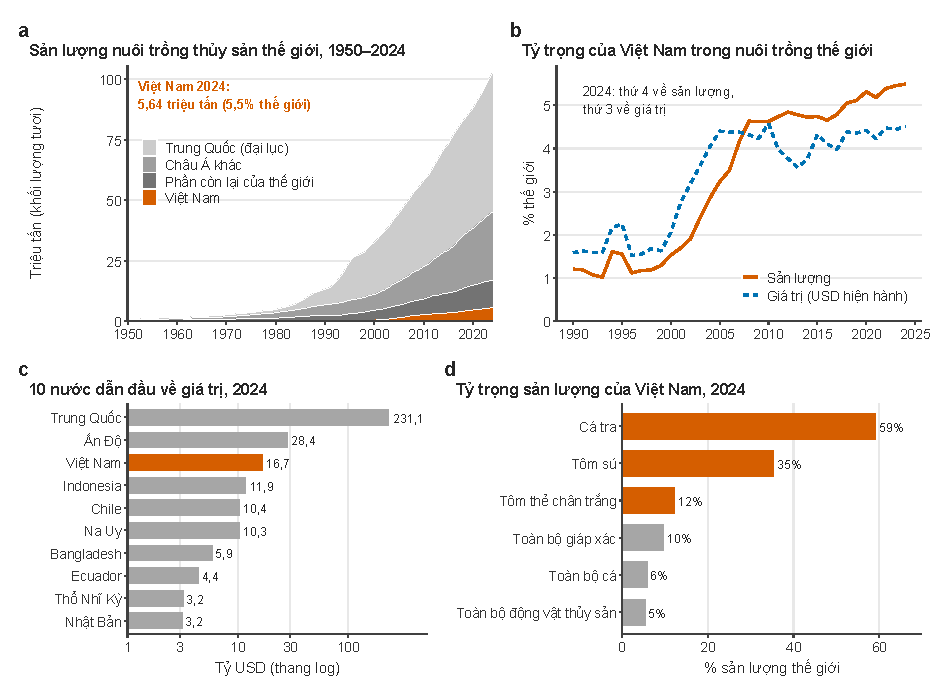
\includegraphics[width=108mm]{jv11_world_aquaculture.pdf}
    \caption{Việt Nam trong ngành nuôi trồng thủy sản thế giới.\\
    \textit{Nguồn:} FAO FishStat, sản lượng nuôi trồng toàn cầu 1950--2024 (bản 2026.1.0); tính toán của tác giả.}
    \label{fig:world}
\end{figure}

Tăng trưởng tuy nhanh nhưng đang chậm lại (Hình~\ref{fig:growth}a). Sản lượng tăng bình quân 13,5\%/năm giai đoạn 1994--2004, 10,8\% giai đoạn 2004--2014 và 5,4\% giai đoạn 2014--2024, so với 7,2\%, 5,3\% và 3,8\% của thế giới. Về giá trị, Việt Nam tăng nhanh hơn thế giới ở thập kỷ đầu và thập kỷ gần nhất, nhưng không nhanh hơn trong 2004--2014, khi giá trị nuôi trồng của Trung Quốc tăng 16\%/năm. Từ giữa thập niên 2010, tôm, nhất là tôm thẻ chân trắng, đã vượt cá tra để trở thành nguồn giá trị chính: năm 2024 tôm thẻ đạt 5,8 tỷ USD, tôm sú 2,7 tỷ USD và cá tra 2,9 tỷ USD (Hình~\ref{fig:growth}c). Số liệu thống kê trong nước cho thấy nguồn gốc của tăng trưởng: giai đoạn 1995--2024, sản lượng tăng khoảng 15 lần trong khi diện tích thu hoạch chỉ tăng 2,5 lần, nên sản lượng trên mỗi hecta tăng từ 0,86 lên 5,26 tấn \parencite{nso_pxweb}. Do đó, tăng trưởng chủ yếu đến từ thâm canh: mỗi hecta ao nuôi nay mang nhiều giá trị hơn, và cũng chịu phơi nhiễm lớn hơn với các hiểm họa trình bày dưới đây. Tổng sản lượng theo FAO và Cục Thống kê chênh nhau không nhiều (5,64 và 5,90 triệu tấn năm 2024); nghiên cứu này dùng FAO khi so sánh quốc tế và Cục Thống kê cho các chuỗi trong nước.

\begin{figure}[!tbp]
    \centering
    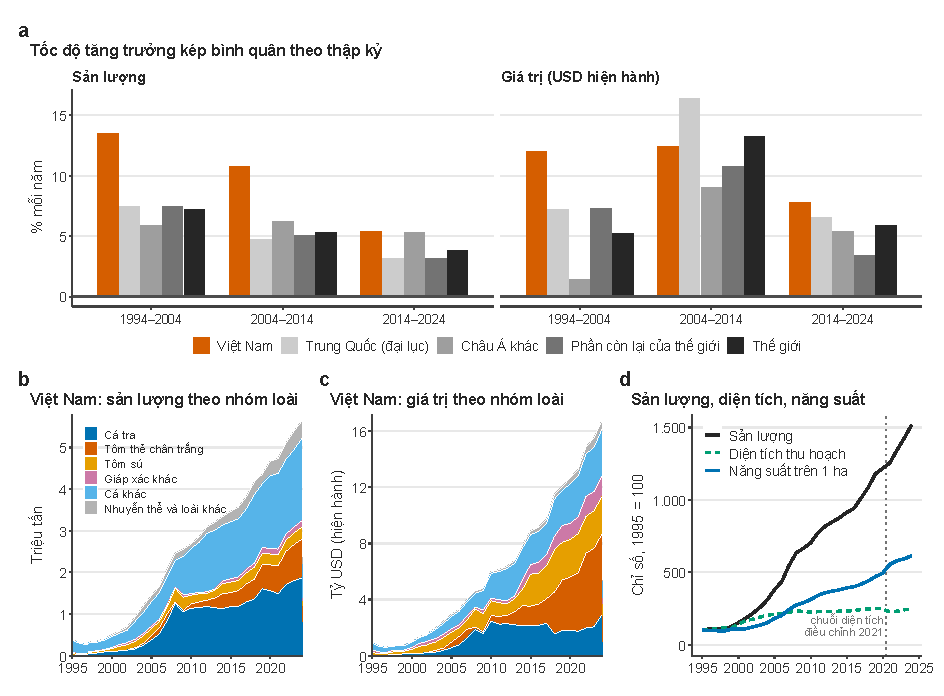
\includegraphics[width=108mm]{jv12_sector_growth.pdf}
    \caption{Tăng trưởng nuôi trồng thủy sản của Việt Nam và thế giới.\\
    \textit{Nguồn:} FAO FishStat 2026.1.0 (a--c); Cục Thống kê (d); tính toán của tác giả.}
    \label{fig:growth}
\end{figure}


\subsection{Hiểm họa thiên tai đang leo thang}

Thiệt hại kinh tế do thiên tai cả nước năm 2024 và 2025 lần lượt là 88.748 và 98.677 tỷ đồng, so với mức trung bình 21 nghìn tỷ đồng giai đoạn 2014--2023, tức gấp hơn bốn lần \parencite{vov2024thientai,nnmt2025thientai}; số cơn bão và áp thấp nhiệt đới trên Biển Đông năm 2025 cao nhất từ 1980 (Hình~\ref{fig:esc}b). Ở ĐBSCL, hiểm họa chính là hạn mặn: EM-DAT ghi 27 lượt tỉnh có hạn hán trong 2000--2022, tăng từ 4 lượt (2000--2011) lên 23 lượt (2012--2022) \parencite{emdat}, và hai đợt hạn mặn 2015--2016, 2019--2020 mỗi đợt phủ 10--13 tỉnh cùng lúc \parencite{nhandan2016hanman,tuoitre2020hanman,cand2020soctrang}. Chính tính hiệp biến này tạo ra rủi ro cơ sở và rủi ro đuôi mà doanh nghiệp bảo hiểm phải gánh (mục~\ref{sec:framework}). Nhiệt độ nước biển ven năm tỉnh thí điểm là hiểm họa thứ ba, được phân tích ở mục~\ref{sec:results}.

\begin{figure}[!tbp]
    \centering
    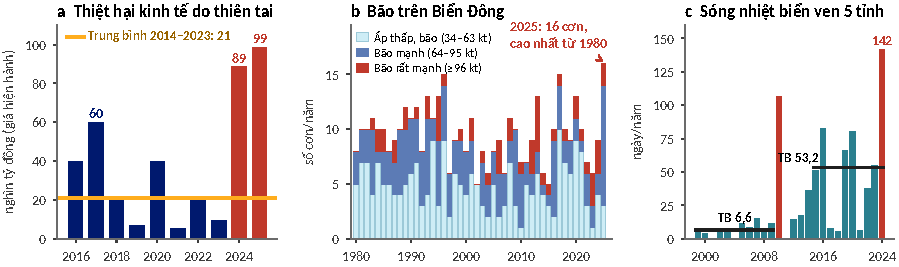
\includegraphics[width=\textwidth]{pb_f1_escalation.pdf}
    \caption{Thiên tai ngày càng dữ dội. (a) Thiệt hại kinh tế do thiên tai cả nước (giá hiện hành). (b) Số cơn bão và áp thấp nhiệt đới có gió từ 34 kt trên Biển Đông, theo cấp. (c) Số ngày sóng nhiệt biển mỗi năm ở vùng biển ven năm tỉnh thí điểm.\\
    \textit{Nguồn:} (a) \textcite{vov2024thientai,nnmt2025thientai} và các báo cáo thiệt hại dẫn trong bảng; (b) IBTrACS v04r01; (c) NOAA OISST \parencite{huang2021oisst}, định nghĩa của \textcite{hobday2016}; tính toán của tác giả.}
    \label{fig:esc}
\end{figure}

\subsection{Khung pháp lý}

Bảo hiểm nông nghiệp được thí điểm theo Quyết định 315/QĐ-TTg ngày 01/3/2011 cho giai đoạn 2011--2013 ở 20 tỉnh, gồm lúa, vật nuôi và thủy sản \parencite{decision315_2011}. Theo số liệu Bộ Tài chính do báo chí dẫn lại, 7.487 hộ tham gia bảo hiểm tôm, cá với tổng phí 218,1 tỷ đồng, trong khi bồi thường lên tới 675,9 tỷ đồng, gấp khoảng 3,1 lần phí; tái bảo hiểm nước ngoài từ chối nhận rủi ro tôm, cá \parencite{tbtc2016bhts}. Thủy sản không được tiếp tục sau thí điểm.

Nghị định 58/2018/NĐ-CP thiết lập khung lâu dài hơn, trong đó, Điều 19 quy định mức hỗ trợ tối đa 90\% cho cá nhân thuộc hộ nghèo, cận nghèo và 20\% cho cá nhân khác và tổ chức đủ điều kiện; Điều 20 liệt kê thiên tai và dịch bệnh có thể được hỗ trợ; Điều 3 đã cho phép các sản phẩm bồi thường theo thiệt hại, theo năng suất, theo chỉ số thời tiết và chỉ số viễn thám \parencite{decree58_2018}. Thủ tướng quyết định cụ thể đối tượng, rủi ro, địa bàn, thời gian. QĐ 22/2019/QĐ-TTg (26/6/2019) hỗ trợ tôm sú, tôm thẻ chân trắng ở năm tỉnh đến hết 2020; QĐ 03/2021/QĐ-TTg kéo dài đến hết 2021 và cập nhật chuẩn nghèo; QĐ 13/2022/QĐ-TTg áp dụng từ 24/6/2022 đến 31/12/2025 và bổ sung cá tra \parencite{decision22_2019,decision03_2021,decision13_2022,tbtc2022qd13}. NĐ 346/2026/NĐ-CP, ký ngày 05/9/2026, nâng trần lên 95/50/30\% và phân cấp cho HĐND tỉnh \parencite{decree346_2026,tckttc2026nd346}.

\subsection{Rủi ro được bảo hiểm và cơ chế kích hoạt}

Điều 5 khoản 3 QĐ 22/2019 quy định thiên tai được hỗ trợ cho tôm gồm bão, áp thấp nhiệt đới, lốc, sét, mưa lớn, lũ, ngập lụt, sạt lở và sụt lún đất do mưa lũ hoặc dòng chảy, nước dâng, \emph{xâm nhập mặn, nắng nóng, hạn hán}, mưa đá, động đất, sóng thần. Kèm theo hai điều kiện: thiên tai phải được công bố hoặc xác nhận của cơ quan nhà nước có thẩm quyền, và không hỗ trợ cho các rủi ro dịch bệnh đối với tôm. QĐ 13/2022 giữ nguyên danh mục này cho tôm và cá tra \parencite{tbtc2022qd13}. Sản phẩm thường được mô tả là chủ yếu bảo hiểm bão, lũ. Độ lệch của chính sách bảo hiểm nằm ở cơ chế kích hoạt và việc loại trừ dịch bệnh.

\subsection{Kết quả triển khai}

Bảng~\ref{tab:phase} tóm tắt hai lần thử và khoảng trống hiện nay.

\begin{table}[!tbp]
\centering\scriptsize
\setlength{\tabcolsep}{3pt}
\caption{Các giai đoạn của bảo hiểm thủy sản có hỗ trợ phí}
\label{tab:phase}
\begin{tabularx}{\textwidth}{@{}>{\raggedright\arraybackslash}p{1.9cm}>{\raggedright\arraybackslash}p{2.7cm}>{\raggedright\arraybackslash}p{3.6cm}>{\raggedright\arraybackslash}p{2.4cm}Y@{}}
\toprule
Giai đoạn & Văn bản & Rủi ro được bảo hiểm & Hỗ trợ phí & Kết quả triển khai \\
\midrule
2011--2013 (thí điểm) & QĐ 315/2011 & Tôm sú, tôm thẻ, cá tra, cá ba sa; thiên tai \emph{và dịch bệnh} & Nghèo 100\%, cận nghèo 80\%, hộ khác 60\% & Có: 7.487 hộ nuôi; phí 218,1 tỷ, bồi thường 675,9 tỷ đồng (3,1 lần) \parencite{tbtc2016bhts}; tỷ lệ bồi thường thủy sản 306\%, lúa 20,6\% \parencite{tnck2014lonang} \\
2014--2018 & Không có chính sách & --- & --- & Năm 2015 Bộ Tài chính đề xuất dừng bảo hiểm thủy sản \parencite{tepbac2015dung} \\
2019--2025 & NĐ 58/2018; QĐ 22/2019, 03/2021, 13/2022 & Tôm (từ 2019), cá tra (từ 6/2022); chỉ thiên tai, không gồm dịch bệnh; nửa đầu 2022 không có văn bản thực hiện & Nghèo, cận nghèo 90\%; hộ khác 20\% & Không: không tỉnh nuôi tôm nào triển khai \parencite{tbtc2025nd58}; cá tra chưa triển khai \parencite{vnplus2026dophu} \\
Từ 20/10/2026 & NĐ 346/2026 & HĐND tỉnh chọn địa bàn, đối tượng, rủi ro; cho phép bảo hiểm chỉ số & Tối đa 95\%, 50\%, 30\% & Chưa có sản phẩm \\
\bottomrule
\end{tabularx}
\begin{minipage}{\textwidth}\footnotesize
\textit{Nguồn:} văn bản pháp luật và các nguồn trích dẫn trong bảng; tổng hợp của tác giả.
\end{minipage}
\end{table}

Số liệu hành chính cho thấy từ 2019 đến đầu 2025, 4/29 địa phương triển khai hỗ trợ: Nghệ An, Thái Bình (lúa) và Hà Giang, Bình Định (trâu, bò); tổng cộng 20.261 hộ, tổ chức tham gia, tổng phí 9,47 tỷ đồng, trong đó ngân sách hỗ trợ 8,02 tỷ \parencite{tbtc2025nd58}. Giai đoạn QĐ 13/2022 có 3.630 hộ tham gia với giá trị bảo hiểm 70,97 tỷ đồng đến đầu 2025; một nguồn khác cho 3.280 hộ và tổng phí 2,38 tỷ đồng \parencite{baodautu2026bhnn,tbtc2026hangnghin}. Không nguồn nào nêu hợp đồng tôm, cá tra được hỗ trợ. Cơ quan quản lý nêu các vướng mắc: thiếu số liệu thiệt hại để xác định phí, mức hỗ trợ thấp, phê duyệt danh sách đối tượng chậm và tái bảo hiểm quốc tế thận trọng \parencite{tbtc2025nd58,tbtc2026hangnghin}.

Hình~\ref{fig:context} đặt các công cụ chính sách này cạnh quá trình tăng trưởng của ngành. Sản lượng nuôi trồng (cộng theo tỉnh) tăng khoảng bốn lần giữa 2005 và 2024, và năm tỉnh thí điểm đóng góp khoảng ba phần tư mức tăng của sản lượng tôm nuôi. Sản phẩm bảo hiểm tôm có trợ cấp có hiệu lực khoảng sáu năm, từ giữa 2019 đến cuối 2025, với khoảng trống trong nửa đầu 2022.

Hình~\ref{fig:pilot} cho thấy vì sao doanh nghiệp rút lui sau thí điểm: bồi thường gấp 3,1 lần phí ở cấp quốc gia, và ở Cà Mau mức phí tôm phải nâng từ 7,42\% lên 13,73\% giá trị bảo hiểm chỉ trong hai năm \parencite{tbtc2016bhts,tepbac2014camau}. Ở Sóc Trăng, Bạc Liêu, bồi thường ước gấp 3--4 lần phí, một phần do khai sai ngày tôm chết \parencite{vnexpress2013tom}. Thí điểm này bảo hiểm cả dịch bệnh, nên không thể suy trực tiếp ra tỷ lệ bồi thường của sản phẩm chỉ có thiên tai từ 2019.

\begin{figure}[!tbp]
    \centering
    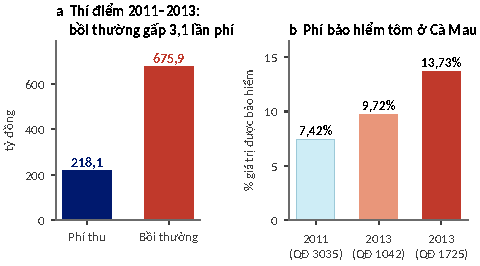
\includegraphics[width=0.55\textwidth]{pb_f4_pilot.pdf}
    \caption{Thí điểm 2011--2013: bồi thường vượt xa phí, và phí phải tăng liên tục. (a) Phí thu và bồi thường toàn chương trình tôm, cá. (b) Tỷ lệ phí bảo hiểm tôm ở Cà Mau theo quyết định của Bộ Tài chính.\\
    \textit{Nguồn:} \textcite{tbtc2016bhts,tepbac2014camau}; số liệu báo chí dẫn lại từ Bộ Tài chính, không phải số liệu chính thức; tính toán của tác giả.}
    \label{fig:pilot}
\end{figure}

\begin{figure}[!tbp]
    \centering
    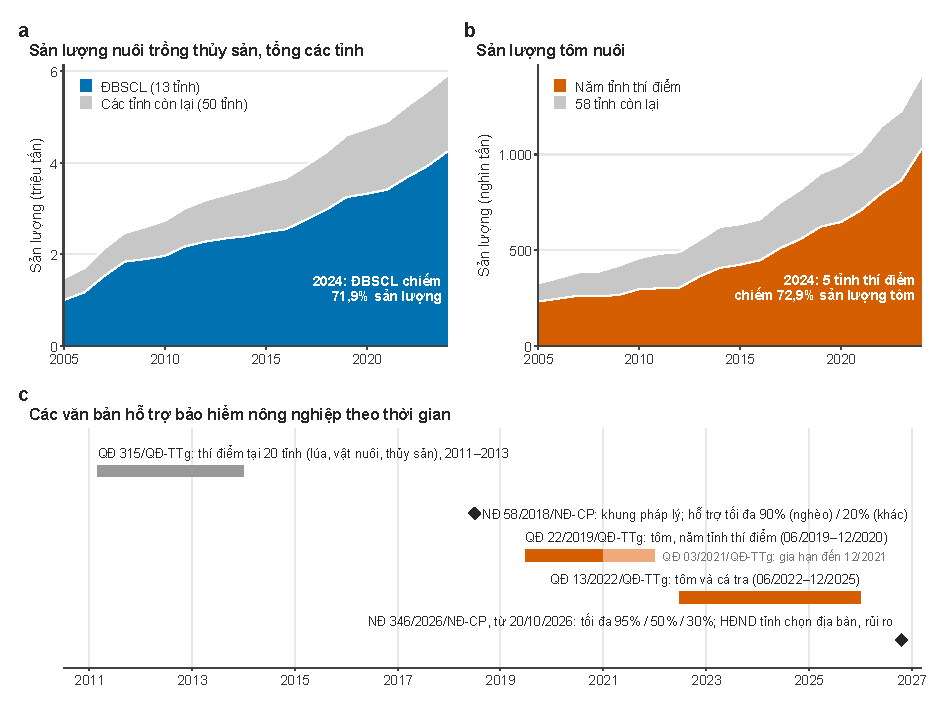
\includegraphics[width=135mm]{jv01_production_policy_timeline.pdf}
    \caption{Sản lượng nuôi trồng thủy sản và các văn bản hỗ trợ bảo hiểm.\\
    \textit{Nguồn:} Cục Thống kê; NĐ 58/2018 và 346/2026; QĐ 315/2011, 22/2019, 03/2021 và 13/2022.}
    \label{fig:context}
\end{figure}

Hình~\ref{fig:gap} đặt quy mô thị trường bảo hiểm cạnh quy mô thiệt hại. Tổng phí bảo hiểm nông nghiệp cả nước 2020--2025, kể cả sản phẩm thương mại, là 271,3 tỷ đồng, bằng khoảng 0,1\% thiệt hại thiên tai của mọi ngành cùng kỳ (261.394 tỷ đồng) \parencite{vnplus2026dophu}; đây là so sánh về bậc độ lớn giữa hai tổng không cùng phạm vi, không phải tỷ lệ bồi thường. Trong VHLSS 2024, chỉ 7/820 hộ nuôi ở năm tỉnh thí điểm nhận tiền từ bất kỳ loại bảo hiểm phi nhân thọ nào.

\begin{figure}[!tbp]
    \centering
    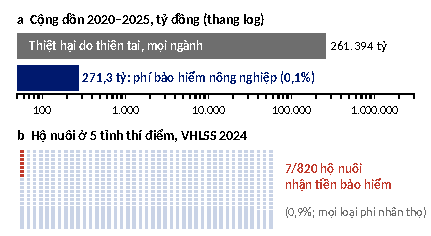
\includegraphics[width=0.7\textwidth]{pb_f7_gap.pdf}
    \caption{Khoảng trống bảo vệ. (a) Thiệt hại do thiên tai (mọi ngành) và phí bảo hiểm nông nghiệp cả nước, cộng dồn 2020--2025, thang log. (b) Hộ nuôi trồng thủy sản ở năm tỉnh thí điểm nhận tiền bảo hiểm trong VHLSS 2024 (mỗi ô là một hộ).\\
    \textit{Nguồn:} thiệt hại như Hình~\ref{fig:esc}a; phí \textcite{vnplus2026dophu}; VHLSS 2024; tính toán của tác giả.}
    \label{fig:gap}
\end{figure}

%====================================================================
\section{Khung lý thuyết}
\label{sec:framework}

\subsection{Cầu bảo hiểm với cơ chế kích hoạt}

Hộ $i$ ở ô rủi ro $z$ chịu tỷ lệ tổn thất $L_i$ trên giá trị bảo hiểm $V$. Tách tổn thất thành phần do rủi ro thuộc danh mục ($L^{c}_i$) và phần do rủi ro ngoài danh mục như dịch bệnh, giá, quản lý ($L^{u}_i$). Với sản phẩm bồi thường hiện hành, chi trả là
\begin{equation}
I_i = A_{zt}\,\max\big(L^{c}_i - d,\,0\big)\,V, \qquad \Pr(A_{zt} = 1 \mid H_{zt}) = \phi(H_{zt}),
\label{eq:trigger}
\end{equation}
trong đó $d$ là mức khấu trừ và $A_{zt}$ là sự kiện cơ quan có thẩm quyền công bố hoặc xác nhận thiên tai ở vùng $z$, năm $t$. Hộ có hàm thỏa dụng CRRA $u(\cdot)$, của cải $w$, phí $\pi_z$, tỷ lệ trợ cấp $s_i$ và cứu trợ kỳ vọng $R_i$ sẽ mua bảo hiểm nếu
\begin{equation}
\EV\big[u(w - VL_i + I_i - (1-s_i)V\pi_z)\big] \geq \EV\big[u(w - VL_i + R_i)\big].
\label{eq:demand}
\end{equation}
Ba yếu tố làm giảm giá trị hợp đồng bất kể $s_i$: tỷ trọng tổn thất ngoài danh mục $\EV[L^{u}]/\EV[L]$ lớn; xác suất công bố $\phi$ thấp với hiểm họa mãn tính, cục bộ như hạn mặn, tạo ra ``rủi ro cơ sở hành chính'' tương tự rủi ro cơ sở của bảo hiểm chỉ số \parencite{clarke2016,jensen2016}; và cứu trợ $R_i$ không bị khấu trừ khi hộ có bảo hiểm \parencite{raschky2007,kousky2018}.

\subsection{Định phí và lựa chọn ngược}

Doanh nghiệp chỉ quan sát được tín hiệu nhiễu về loại rủi ro của hộ sẽ định phí hòa vốn trên tập người mua $B_z$:
\begin{equation}
\pi_z = (1+\theta)\,\EV[I_i \mid i \in B_z(\pi_z)] + \kappa\,\big(\mathrm{CVaR}_{q}(I_z) - \EV[I_z]\big),
\label{eq:premium}
\end{equation}
với $\theta$ là phụ phí quản lý và $\kappa$ là giá vốn cho rủi ro đuôi. Khi phí đồng nhất và rủi ro riêng dị biệt, hộ rủi ro thấp rời khỏi thị trường và tỷ số $\EV[I \mid B]/\EV[I]$ lớn hơn 1 \parencite{rothschild1976,just1999}; phân vùng chính xác hơn làm tỷ số này giảm. Ở phía cung, nếu doanh nghiệp không ước lượng được $\EV[I_z]$ hoặc không tái bảo hiểm được phần đuôi, sản phẩm sẽ không được chào bán ở bất kỳ mức trợ cấp nào.

\subsection{Giả thuyết kiểm định}

(H1) Tổn thất quan trọng với hộ nuôi khó được dự báo bởi các hiểm họa thuộc danh mục và đo được. (H2) Tỷ lệ tham gia và nhận chi trả không phản ứng với chính sách, nên tác động lên sản lượng xấp xỉ 0. (H3) Khác biệt rủi ro không gian quan sát được trong ĐBSCL đủ lớn để định phí theo ô. (H4) Với cùng ngân sách, trợ cấp lũy tiến kết hợp phí theo rủi ro cho độ phủ trên mỗi đồng trợ cấp cao hơn nâng trợ cấp cào bằng.

%====================================================================
\section{Dữ liệu}
\label{sec:data}

\subsection{Dữ liệu hộ}

Nghiên cứu này lấy dữ liệu từ 12 vòng VHLSS (từ 2002 đến 2024), gồm 221.359 lượt hộ. Bảng hỏi về thủy sản ghi nhận giá trị sản lượng theo sản phẩm, sản lượng thu hoạch, chi phí và đền bù thiệt hại thủy sản; mô-đun thu chuyển giao ghi nhận cứu trợ thiên tai của Nhà nước và chi trả bảo hiểm phi nhân thọ. Phiếu xã ghi lũ, bão, hạn và dịch bệnh vật nuôi trong 12 tháng trước phỏng vấn. Mẫu quan sát sau khi lọc và làm sạch gồm: 21.726 lượt hộ có thủy sản ở 34 tỉnh ven biển và ĐBSCL, trong đó 11.792 lượt hộ nuôi trồng và 3.961 lượt hộ nuôi tôm; 22.615 lượt hộ nối được với vòng trước và 5.510 hộ được quan sát 3--4 vòng.

Bốn đặc điểm đo lường định hình thiết kế: (i) câu 1b mô-đun 4B5 chỉ hỏi hộ \emph{không} nuôi trong 12 tháng nên không phải biến tự báo thiệt hại; (ii) mục đền bù 4B5T2 chỉ có từ 2018 và gộp hỗ trợ Nhà nước với tiền bảo hiểm; (iii) mã 108 gồm mọi loại bảo hiểm phi nhân thọ và phí bảo hiểm không được ghi riêng; (iv) chi phí chỉ tính cho sản phẩm đã thu hoạch nên vụ mất trắng không hiện ra như khoản lỗ. Vì vậy VHLSS đo việc \emph{nhận tiền}, không đo việc tham gia (Bảng~\ref{tab:vhlss_n}).

\begin{table}[!tbp]
\centering\scriptsize
\caption{Số hộ nuôi tôm trong VHLSS theo nhóm tỉnh và vòng khảo sát (không trọng số)}
\label{tab:vhlss_n}
\setlength{\tabcolsep}{3.2pt}
\begin{tabular}{@{}lrrrrrrrrrrr@{}}
\toprule
 & 2002 & 2004 & 2006 & 2008 & 2010 & 2012 & 2014 & 2018 & 2020 & 2022 & 2024 \\
\midrule
5 tỉnh thí điểm & 426 & 133 & 139 & 150 & 142 & 327 & 147 & 132 & 635 & 116 & 636 \\
4 tỉnh đối chứng chính & 20 & 11 & 11 & 19 & 8 & 34 & 14 & 22 & 107 & 13 & 73 \\
4 tỉnh ĐBSCL khác & 14 & 7 & 8 & 3 & 2 & 9 & 5 & 2 & 10 & 3 & 4 \\
Phần còn lại & 316 & 88 & 93 & 109 & 73 & 147 & 60 & 58 & 161 & 19 & 103 \\
\midrule
Tổng số hộ của vòng & 29.532 & 9.188 & 9.189 & 9.189 & 9.399 & 23.235 & 9.399 & 9.396 & 47.040 & 9.398 & 46.995 \\
\bottomrule
\end{tabular}
\begin{minipage}{\textwidth}\footnotesize
\textit{Nguồn:} VHLSS; tính toán của tác giả.
\end{minipage}
\end{table}

\subsection{Dữ liệu hiểm họa}

Phơi nhiễm bão đo từ IBTrACS \parencite{knapp2010}: trường gió Rankine cải biên trên lưới 0,1° cho chỉ số phá hủy bậc ba và xác suất có gió $\geq$34 kt \parencite{emanuel2005,strobl2011}. Mưa từ CHIRPS 0,05° \parencite{funk2015}, nhiệt độ tối đa và tối thiểu từ NASA POWER 0,5° \parencite{sparks2018}, hạn từ SPEI-3, SPEI-6 với chuẩn 1991--2020 \parencite{vicente2010}, tất cả gộp về 706 huyện theo tháng giai đoạn 1991--2024. Độ mặn không được quan trắc trực tiếp; mưa mùa khô, đợt khô dài nhất và SPEI là các proxy. Với hộ, hiểm họa được đo trong 12 tháng trước tháng phỏng vấn, theo huyện từ 2010 và theo tỉnh cho 2002--2008.

Một chỉ số gộp bằng PCA chỉ giải thích 24,1\% phương sai và các thành phần mưa--lũ, khô--nóng mang dấu ngược nhau. Nghiên cứu này vì vậy dựng hai chỉ số: $H^{wet}$ (ngày mưa $\geq$50 mm, mưa ngày lớn nhất, dị thường mưa 12 tháng, lũ và bão do xã báo cáo, chỉ số phá hủy bão) và $H^{dry}$ (ngày $T_{\max}\geq$35°C, $T_{\max}$ trung bình, SPEI-3 nhỏ nhất, mưa mùa khô, hạn do xã báo cáo). Thành phần chính thứ nhất của phần lưới giải thích 73,1\% và 55,6\% phương sai; tương quan giữa hai chỉ số là $-0{,}36$. Phiên bản theo mùa chia năm thành mùa D (tháng 1--6, vụ tôm chính theo lịch thời vụ giả định) và mùa W (tháng 7--12). Hiệu ứng cố định tỉnh $\times$ năm hấp thụ 71\% biến thiên của $H^{wet}$ và 68\% của $H^{dry}$.

Nhiệt độ mặt nước biển ven bờ lấy từ phân tích ngày NOAA OISST v2.1 độ phân giải 0,25° \parencite{huang2021oisst}, lấy trung bình trên các ô biển trong phạm vi 50 km quanh mỗi tỉnh ven biển giai đoạn 1999--2024 (dữ liệu 1992--1998 tải về không đủ ngày nên bị loại). Ngày sóng nhiệt biển là ngày thuộc đợt từ 5 ngày liên tiếp trở lên có nhiệt độ vượt phân vị 90 của khí hậu theo ngày trong năm \parencite{hobday2016}.

\subsection{Panel tỉnh}

Sản lượng nuôi trồng tỉnh (tổng, tôm, cá) từ 2005--2024 lấy từ Cục Thống kê \parencite{nso_pxweb}; sự kiện thiên tai EM-DAT chỉ dùng để kiểm định \parencite{emdat}.

%====================================================================
\section{Chiến lược ước lượng}
\label{sec:strategy}

\textbf{Bước một.} Tính tỷ lệ hộ nuôi nhận chi trả bảo hiểm, đền bù thủy sản và cứu trợ Nhà nước theo nhóm tỉnh và vòng, kèm khoảng tin cậy Wilson 95\%, và ước lượng DiD cấp huyện trên các biến này.

\textbf{Tác động lên sản lượng.} Ở cấp tỉnh, ước lượng SDID \parencite{arkhangelsky2021} cho log tổng sản lượng, tôm, cá, coi năm tỉnh là can thiệp từ 2019, với hai tập đơn vị cho: 8 tỉnh ĐBSCL còn lại và 29 tỉnh ven biển và ĐBSCL. Kiểm định độ vững gồm placebo giả định áp dụng 2015 trên mẫu 2005--2018, loại 2011--2013, biến kết quả hiệu chỉnh khí hậu và bỏ lần lượt từng tỉnh. MDE bằng 2,8 lần sai số chuẩn placebo. Do tham gia gần bằng 0, đây là ước lượng ITT làm cận trên cho tác động của chương trình như đã được thực thi, không phải tác động của bảo hiểm lên hộ tham gia. Nghiên cứu này cũng ước lượng nghiên cứu sự kiện so với tám tỉnh ĐBSCL còn lại (với tôm: bốn tỉnh nuôi từ 1.000 tấn/năm trở lên trước 2019) và suy luận hoán vị trên toàn bộ 1.287 cách gán năm tỉnh can thiệp trong 13 tỉnh.

\textbf{Hiểm họa và sản lượng hộ.}
\begin{equation}
y_{ict} = \alpha_c + \lambda_{p(c)t} + \beta^{wet} H^{wet}_{ct} + \beta^{dry} H^{dry}_{ct} + \bm{X}_{ict}'\bm\delta + \varepsilon_{ict},
\label{eq:hh}
\end{equation}
với $y$ là asinh của giá trị sản lượng (triệu đồng), $\alpha_c$ hiệu ứng cố định xã, $\lambda_{p(c)t}$ hiệu ứng cố định tỉnh (hoặc vùng) $\times$ năm, $\bm{X}$ gồm tuổi, giới, học vấn chủ hộ, quy mô hộ, tỷ lệ phụ thuộc; sai số cụm theo xã. Đặc tả theo mùa dùng các chỉ số lệch mùa làm placebo; mô hình xác suất tuyến tính cho quyết định ngừng nuôi ước lượng trên hộ panel.

\textbf{Định phí.} Với sản phẩm minh họa chỉ số sản lượng tỉnh $I_{pt} = \max(0;\ 0{,}9 - Q_{pt}/\hat Q_{pt})$ ($\hat Q$ là xu hướng bậc hai loại năm $t$), nghiên cứu này tính phí thuần thô, CVaR$_{95}$ chính xác, phí theo độ tin cậy Bühlmann--Straub \parencite{buhlmann2005} và đuôi GPD gộp \parencite{embrechts1997,mcneil2015,acerbi2002}.

\textbf{Kiểm định độ vững.} Mỗi nhóm kết quả có một bộ kiểm định riêng (Bảng~\ref{tab:robustplan}): với panel tỉnh, bỏ từng tỉnh, suy luận hoán vị và đặc tả thay thế vì chỉ có 32--34 cụm; với đánh giá chương trình, placebo thời gian, suy luận ngẫu nhiên hóa trên mọi cách gán 5 trong 13 tỉnh và SDID bỏ từng đối chứng vì chỉ có 5 tỉnh được can thiệp; với hộ, đường cong đặc tả, cụm theo xã, huyện và tỉnh, hoán vị trong tỉnh-năm và kiểm định tương đương (TOST) để phân biệt ``không hiệu ứng với ``không đủ lực; với AUC, bootstrap theo cụm tỉnh-năm. Kiểm định tương đương dùng biên $\delta=0{,}20$ do tác giả chọn. Kết quả ở Mục~\ref{sec:robust}.

\textbf{Mô phỏng.}  Monte Carlo 6.000 hộ giải phương trình~\eqref{eq:premium} bằng lặp điểm bất động có giảm chấn, theo các cấu trúc thông tin (phí đồng nhất, theo tỉnh, theo ô với độ chính xác bản đồ $\rho$) và các mức trợ cấp. Tham số là giả định, mô phỏng chưa có cơ chế kích hoạt và cứu trợ; chỉ dùng để xếp hạng thiết kế.

%====================================================================
\section{Kết quả}
\label{sec:results}

\subsection{Hiểm họa ở đâu}

Hình~\ref{fig:map} cho thấy địa lý của bão và địa lý của tôm lệch nhau. Giai đoạn 1980--2023, chỉ 3,8\% tỉnh-năm ở ĐBSCL có gió $\geq$34 kt, so với 49,2\% ở 21 tỉnh ven biển khác. Trong EM-DAT 2000--2022, ĐBSCL có 27 tỉnh-năm hạn hán, so với 9 ở tất cả tỉnh ven biển còn lại. Trên panel tỉnh, một cơn bão chuẩn gắn với sản lượng tôm thấp hơn ($-0{,}53$ log năm $t$ và $-0{,}82$ năm $t-1$ trong Bảng~\ref{tab:twfe}; chạy lại trên bộ dữ liệu đóng gói cho $-0{,}36$ năm $t$, xem Mục~\ref{sec:robust}), nhưng hệ số được nhận dạng gần như hoàn toàn từ ngoài ĐBSCL (13 tỉnh ĐBSCL chỉ đóng góp 3,1\% phương sai phần dư của biến phơi nhiễm) và không có ý nghĩa với wild cluster bootstrap ($p = 0{,}23$ và $0{,}18$; Bảng~\ref{tab:twfe} ở Phụ lục).

\begin{figure}[!tbp]
    \centering
    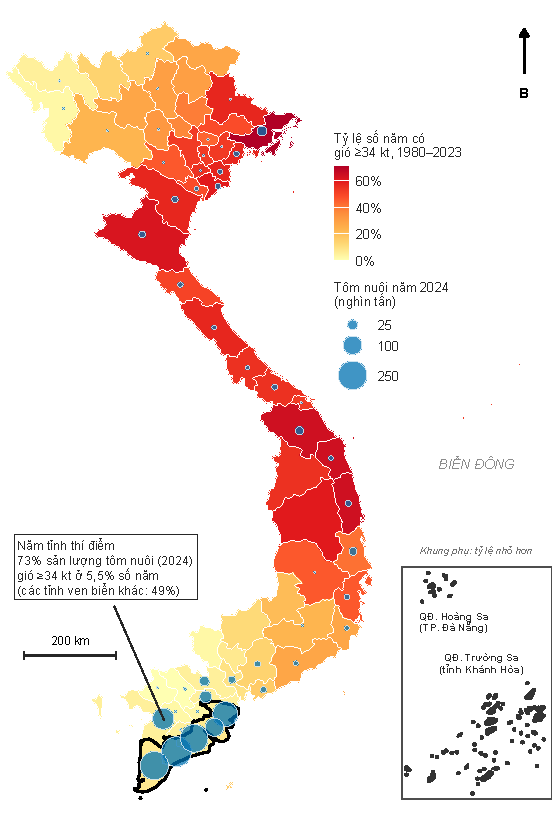
\includegraphics[width=95mm]{jv02_cyclone_shrimp_map.pdf}
    \caption{Hiểm họa bão và sản lượng tôm theo tỉnh.\\
    \textit{Nguồn:} IBTrACS v04 với trường gió Rankine điều chỉnh; Cục Thống kê; geoBoundaries; tính toán của tác giả.}
    \label{fig:map}
\end{figure}

Hình~\ref{fig:tracks} đặt đường đi của 168 cơn bão có gió từ 34 kt trở lên ở Việt Nam, 1980--2026, cạnh xác suất năm có gió ấy theo tỉnh. Mười cơn bão đi trong phạm vi 150 km quanh năm tỉnh thí điểm là DURIAN (2006, 135 kt), MUIFA (2004), ANGELA (1992), USAGI (2018), TEMBIN (2017), TERESA (1994), LINDA (1997), PAKHAR (2012), FORREST (1992) và CHIP (1998). Trong 44 năm, mỗi tỉnh thí điểm có gió từ 34 kt trong khoảng 4,5--6,8\% số năm, trung bình 5,5\% tỉnh-năm, tức là khoảng hai đến ba năm mỗi tỉnh. Xác suất này thấp hơn nhiều so với 49\% ở các tỉnh ven biển khác, nên bão ít đe dọa trực tiếp ĐBSCL. Khi bão đến, tuy vậy, tổn thất dồn vào cùng một vùng, và vì thế rủi ro này khó chia sẻ trong phạm vi xã.

\begin{figure}[!tbp]
    \centering
    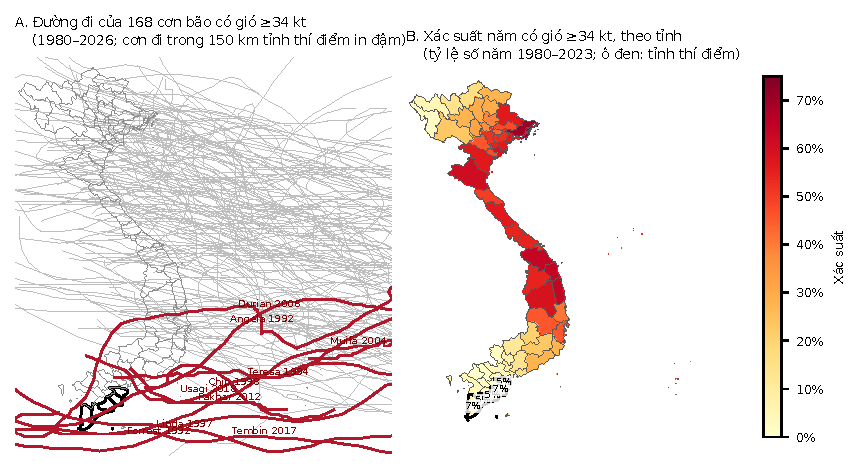
\includegraphics[width=\textwidth]{jv15_tc_tracks_probability.pdf}
    \caption{Đường đi bão và xác suất gió mạnh theo tỉnh. (a) Đường đi của 168 cơn bão có gió từ 34 kt trở lên ở Việt Nam, 1980--2026; màu đỏ: cơn đi trong phạm vi 150 km quanh năm tỉnh thí điểm, kèm tên và năm. (b) Tỷ lệ số năm 1980--2023 mà một phần tỉnh có gió từ 34 kt; ô đen: tỉnh thí điểm, số ghi là tỷ lệ của tỉnh. Phạm vi 150 km là chỉ dẫn đơn giản về bán kính gió, không thay cho trường gió của từng cơn bão. \textit{Nguồn:} IBTrACS v04r00 (trường gió Rankine điều chỉnh); geoBoundaries; tính toán của tác giả.}
    \label{fig:tracks}
\end{figure}

Trong ĐBSCL, hiểm họa khí tượng biến thiên đáng kể giữa 132 huyện (Hình~\ref{fig:gis}): 0--101 ngày/năm có $T_{\max}>35$°C, đợt khô dài nhất 26--68 ngày, mưa 5 ngày lớn nhất 87--211 mm. Các chỉ số tập trung thành cụm rõ rệt (Moran's $I$ 0,76--0,81; $p<0{,}001$) và 24--32\% biến thiên nằm trong tỉnh. Phân vùng liên thông SKATER \parencite{assuncao2006} với 5 ô giải thích 73\% phương sai đa biến, gần bằng 13 tỉnh (80\%), và cắt ngang năm tỉnh, trong đó có hai tỉnh thí điểm; 43/44 huyện thí điểm thuộc hai ô ven biển. Hiểm họa khí tượng đo được từ vệ tinh chủ yếu khác nhau giữa các tỉnh; lập luận cho phân vùng dưới cấp tỉnh phải dựa vào độ mặn và dịch bệnh, vốn chưa có bản đồ.

\begin{figure}[!tbp]
    \centering
    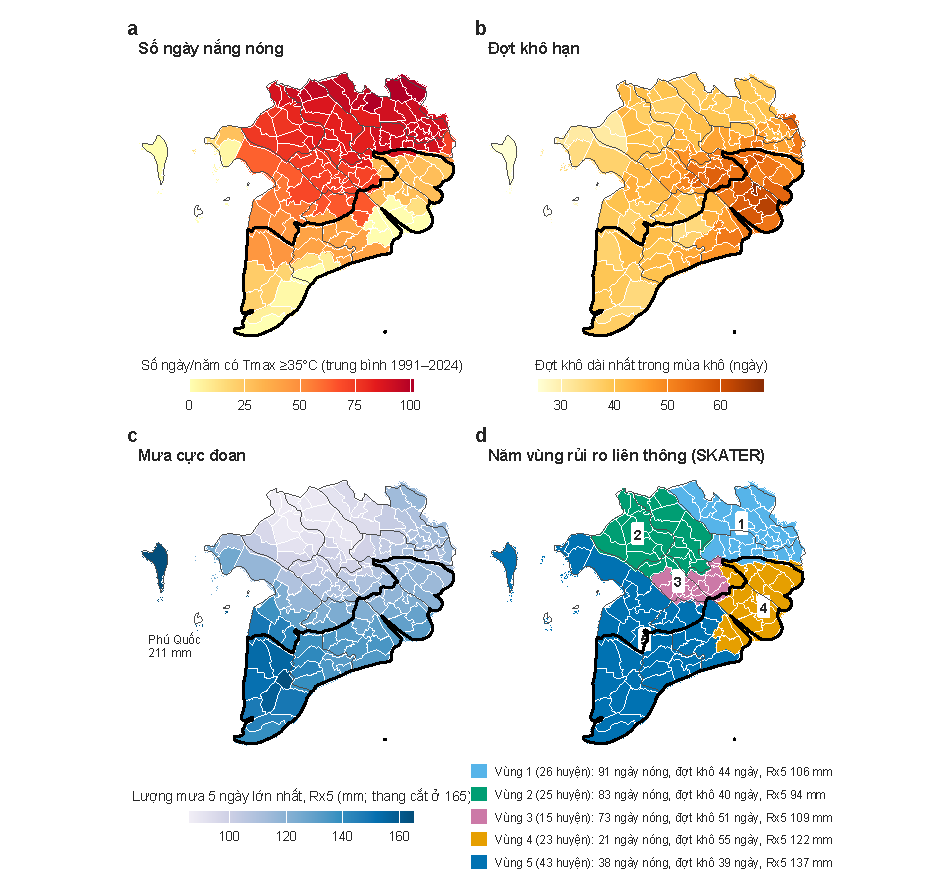
\includegraphics[width=150mm]{jv03_mekong_hazard_zones.pdf}
    \caption{Hiểm họa khí tượng ở 132 huyện ĐBSCL, trung bình 1991--2024. (a) Số ngày/năm có nhiệt độ tối đa từ 35°C. (b) Đợt khô hạn dài nhất trong mùa khô. (c) Lượng mưa 5 ngày lớn nhất; thang màu cắt ở mức cao nhất trên đất liền (165 mm) và đảo Phú Quốc (211 mm) được ghi nhãn riêng. (d) Năm vùng rủi ro liên thông theo phân vùng SKATER \parencite{assuncao2006} trên bốn chỉ số chuẩn hóa (ngày nắng nóng, đợt khô, Rx5 và xác suất bão); chú giải nêu đặc trưng trung bình của từng vùng, số vùng ghi trên bản đồ. Đường xám mảnh: ranh giới tỉnh; đường đen đậm: tỉnh thí điểm.\\
    \textit{Nguồn:} CHIRPS; NASA POWER (37 huyện không có ô lưới lấy giá trị huyện gần nhất); IBTrACS; geoBoundaries; tính toán của tác giả.}
    \label{fig:gis}
\end{figure}

\subsection{Hiểm họa có đang thay đổi?}

Trên đất liền, chuỗi cấp huyện 1991--2024 không có xu thế vững nào (Hình~\ref{fig:clim}). Xu thế trung vị của số ngày có nhiệt độ tối đa từ 35°C là $-0{,}4$ ngày mỗi thập kỷ, chỉ dương và có ý nghĩa ở mức 5\% tại 4,5\% số huyện; nhiệt độ tối đa mùa nóng tăng trung vị 0,14°C mỗi thập kỷ nhưng chỉ có ý nghĩa ở 2\% số huyện; không huyện nào có xu thế ý nghĩa của lượng mưa mùa khô (tháng 12--4). Biến động giữa các năm chiếm ưu thế: xếp theo SPEI-3 nhỏ nhất trung bình toàn vùng, năm năm khô nhất là 1997, 2016, 2002, 2024 và 2015.

Ngược lại, rủi ro nhiệt đang tăng nhanh ở biển ven bờ. Ở vùng biển trong phạm vi 50 km quanh năm tỉnh thí điểm, dị thường nhiệt độ mặt nước biển tăng 0,30°C mỗi thập kỷ, và số ngày sóng nhiệt biển tăng từ 6,6 ngày/năm giai đoạn 1999--2009 lên 53,2 ngày/năm giai đoạn 2015--2024, đạt 142 ngày năm 2024.

\begin{figure}[!tbp]
\centering
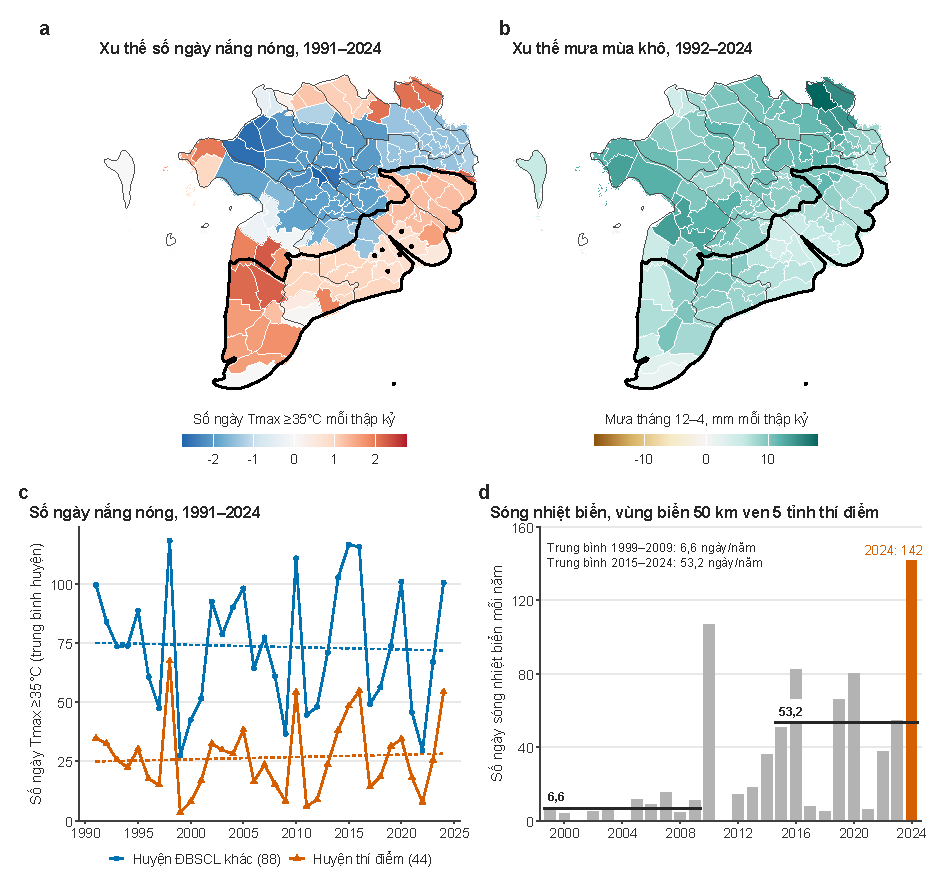
\includegraphics[width=150mm]{jv04_climate_trends.pdf}
\caption{Xu thế khí hậu ở ĐBSCL. (a) Xu thế OLS cấp huyện của số ngày nhiệt độ tối đa $\geq$35°C, 1991--2024; (b) xu thế mưa tháng 12--4, 1992--2024; chấm: huyện có $p<0{,}05$. (c) Số ngày nắng nóng trung bình huyện, huyện thí điểm và huyện ĐBSCL khác, kèm đường xu thế. (d) Số ngày sóng nhiệt biển mỗi năm ở vùng biển trong phạm vi 50 km quanh năm tỉnh thí điểm, 1999--2024 (đợt $\geq$5 ngày vượt phân vị 90 của khí hậu theo ngày 1991--2020, tính trên các năm có dữ liệu \parencite{hobday2016}); đường ngang là trung bình 1999--2009 và 2015--2024. Ở (a) và (b), thang màu phân kỳ theo quy ước IPCC (đỏ--xanh cho nhiệt độ, nâu--xanh lục cho lượng mưa), đối xứng quanh 0. Viền đen: tỉnh thí điểm. \textit{Nguồn:} CHIRPS; NASA POWER (37 huyện lấy giá trị huyện gần nhất); NOAA OISST v2.1 \parencite{huang2021oisst}; tính toán của tác giả.}
\label{fig:clim}
\end{figure}

Kết luận không xu thế trên đất liền cần đọc thận trọng vì hai lý do. Ba mươi tư năm là ngắn để phát hiện xu thế trong chuỗi cấp huyện nhiều nhiễu, và 37 huyện mượn số liệu nhiệt độ của huyện lân cận, nên việc không thấy xu thế trên đất liền không chứng minh rủi ro ổn định. Ngưỡng sóng nhiệt biển không gồm các năm 1992--1998, nên ngưỡng có thể cao hơn đôi chút nếu các năm đó mát. Dù vậy, hàm ý cho thiết kế bảo hiểm là trực tiếp: với nhiệt độ nước ven biển, yếu tố quan trọng với ao lấy nước biển, các năm gần đây không còn là mẫu rút từ phân phối 1991--2020, và phí hay ngưỡng kích hoạt hiệu chỉnh theo khí hậu đó sẽ đánh giá thấp mức phơi nhiễm hiện nay.

Chi trả bảo hiểm gần như vắng mặt trong dữ liệu: hộ nuôi ở tỉnh thí điểm nhận chi trả chưa bao giờ vượt 1,1\% (cao nhất là 2/195 năm 2018), và không có bước nhảy sau 2019 hay 2022 (Bảng~\ref{tab:firststage}, Hình~\ref{fig:first}). Năm 2020, vòng có mẫu lớn nhất, không hộ nào trong 890 hộ nuôi ở năm tỉnh nhận chi trả hay đền bù (cận trên KTC 95\% là 0,4\%). Tỷ lệ năm 2024 (7/820; 0,9\%, KTC 0,4--1,8\%) không cao hơn tỉnh đối chứng (5/285; 1,8\%); DiD cấp huyện trên biến nhận chi trả cho $-0{,}014$ (SE 0,012). Năm 2022, cứu trợ Nhà nước đến với 19/169 hộ nuôi ở tỉnh thí điểm (11\%) trong khi bảo hiểm bằng 0: khi tổn thất xảy ra, Nhà nước chứ không phải doanh nghiệp bảo hiểm là bên chi trả.

Tỷ lệ nhận chi trả bằng tích của xác suất tham gia và xác suất sự kiện được bồi thường xảy ra trong kỳ hồi tưởng, nên tỷ lệ thấp tự nó chưa chứng minh tham gia thấp. Hai dữ kiện trong bảng cho phép loại bỏ cách giải thích chỉ do không có tổn thất. Thứ nhất, cứu trợ Nhà nước đến với 11\% hộ thí điểm năm 2022, nên sự kiện thiên tai đủ lớn để kích hoạt can thiệp công là phổ biến trong kỳ hồi tưởng. Thứ hai, ở năm 2020 và năm 2022 không hộ nào trong tổng 1.059 hộ nuôi ở năm tỉnh nhận chi trả bảo hiểm. Để minh họa bằng số học (không phải ước lượng): nếu tỷ lệ tham gia là 56\% như mô phỏng khung hiện hành (giả định) và xác suất được bồi thường của người tham gia chỉ bằng một nửa tần suất cứu trợ 11\%, tỷ lệ nhận chi trả kỳ vọng vẫn khoảng 3\%, tức hàng chục hộ trong mẫu 890 hộ năm 2020. Kết quả quan sát bằng 0 vì vậy phù hợp với tham gia rất thấp, hoặc với chi trả hầu như không bao giờ được kích hoạt cho người tham gia (VHLSS không phân biệt được hai khả năng này, và đây là lý do nghiên cứu này kết luận về \emph{độ phủ thực tế} chứ không về cầu).

\begin{table}[!tbp]
\centering\scriptsize
\caption{Số hộ nuôi trồng thủy sản nhận chi trả bảo hiểm, đền bù và cứu trợ (VHLSS)}
\label{tab:firststage}
\setlength{\tabcolsep}{3.4pt}
\begin{tabular}{@{}lrrrrrrrrrr@{}}
\toprule
 & 2004 & 2006 & 2008 & 2010 & 2012 & 2014 & 2018 & 2020 & 2022 & 2024 \\
\midrule
\multicolumn{11}{@{}l}{\textit{A. Chi trả bảo hiểm phi nhân thọ (4D mã 108; mã 105 năm 2004)}} \\
5 tỉnh thí điểm & 0/221 & 0/249 & 1/268 & 0/233 & 1/494 & 1/197 & 2/195 & 0/890 & 0/169 & 7/820 \\
4 tỉnh đối chứng & 1/190 & 0/166 & 0/147 & 1/115 & 0/225 & 0/117 & 0/112 & 1/364 & 0/63 & 5/285 \\
Phần còn lại & 14/1.070 & 7/1.008 & 7/949 & 1/798 & 0/1.669 & 3/630 & 0/662 & 17/2.252 & 3/416 & 15/1.995 \\
\midrule
\multicolumn{11}{@{}l}{\textit{B. Đền bù, hỗ trợ thiệt hại thủy sản (4B5T2, từ 2018)}} \\
5 tỉnh thí điểm & & & & & & & 2/195 & 0/890 & 0/169 & 1/820 \\
4 tỉnh đối chứng & & & & & & & 0/112 & 0/364 & 0/63 & 0/285 \\
Phần còn lại & & & & & & & 9/662 & 26/2.252 & 2/416 & 6/1.995 \\
\midrule
\multicolumn{11}{@{}l}{\textit{C. Cứu trợ thiên tai, dịch bệnh của Nhà nước (4D mã 107)}} \\
5 tỉnh thí điểm & & 0/249 & 2/268 & 0/233 & 2/494 & 1/197 & 0/195 & 2/890 & 19/169 & 0/820 \\
4 tỉnh đối chứng & & 0/166 & 0/147 & 0/115 & 1/225 & 9/117 & 0/112 & 8/364 & 10/63 & 0/285 \\
Phần còn lại & & 24/1.008 & 84/949 & 53/798 & 40/1.669 & 9/630 & 8/662 & 33/2.252 & 7/416 & 12/1.995 \\
\bottomrule
\end{tabular}
\begin{minipage}{\textwidth}\footnotesize
\textit{Ghi chú:} Số hộ có giá trị dương / số hộ nuôi trồng thủy sản trong mẫu. \textit{Nguồn:} VHLSS; tính toán của tác giả.
\end{minipage}
\end{table}

\begin{figure}[!tbp]
\centering
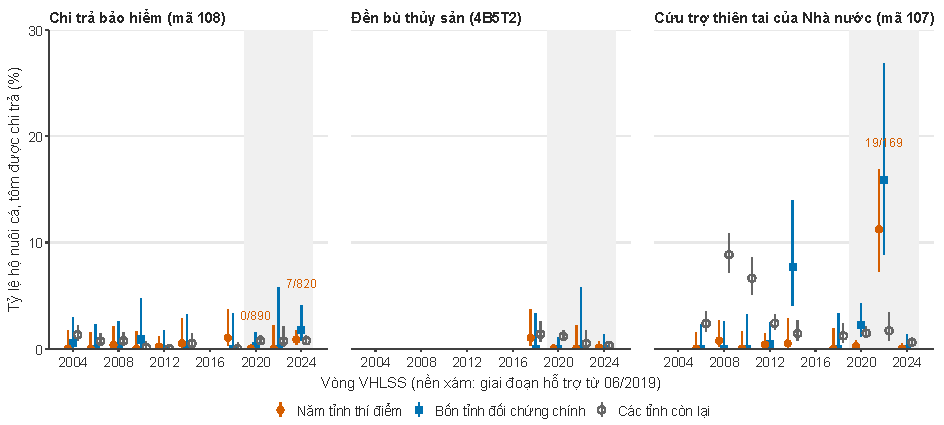
\includegraphics[width=122mm]{jv05_first_stage.pdf}
\caption{Bước một: tỷ lệ hộ nuôi cá, tôm nhận từng loại chi trả theo vòng VHLSS và nhóm tỉnh, không gia quyền, KTC Wilson 95\%. Chi trả bảo hiểm (mã thu nhập 108) gồm mọi loại bảo hiểm phi nhân thọ; đền bù thủy sản (phần 4B5T2) chỉ có từ 2018 và gộp hỗ trợ Nhà nước với bảo hiểm; cứu trợ thiên tai của Nhà nước là mã 107 (từ 2006). Nền xám: các vòng sau khi bắt đầu hỗ trợ tôm (06/2019). Nhãn ghi số hộ của năm tỉnh thí điểm (hộ được chi trả/hộ nuôi). Bốn tỉnh ĐBSCL còn lại không vẽ do mẫu nhỏ. \textit{Nguồn:} VHLSS 2004--2024; tính toán của tác giả.}
\label{fig:first}
\end{figure}

\subsection{Tác động của chương trình lên sản lượng}

Tác động lên sản lượng tỉnh gần bằng 0 ở mọi đặc tả, và mọi khoảng tin cậy đều chứa 0 (Bảng~\ref{tab:did}). Với tập đơn vị cho rộng, ước lượng cho tổng sản lượng là 0,016 (SE 0,066), loại trừ tác động lớn hơn khoảng 0,18 log (khoảng 20\%); cho tôm là 0,110 (SE 0,115), nhưng placebo áp dụng 2015 cho 0,090, nghĩa là chênh lệch là quá trình đuổi kịp có từ trước. DiD hai chiều thông thường cho tôm (0,380) gấp đôi placebo của nó (0,164). Với tập 8 tỉnh ĐBSCL, MDE của tôm vượt 2 log nên thiết kế này không cho thông tin. Suy luận hoán vị trên 1.287 cách gán cho $p=0{,}96$ với tổng sản lượng. Hình~\ref{fig:sdid}a so sánh các ước lượng với tác động tối thiểu phát hiện được.

\begin{table}[!tbp]
\centering\footnotesize
\setlength{\tabcolsep}{4pt}
\caption{Tác động của chương trình lên log sản lượng tỉnh: SDID, placebo và MDE, 2005--2024}
\label{tab:did}
\begin{tabular}{@{}llccccc@{}}
\toprule
Biến kết quả & Đơn vị cho & SDID (SE) & Placebo 2015 (SE) & Hiệu chỉnh KH & MDE & Số tỉnh cho \\
\midrule
Tổng sản lượng & 8 tỉnh ĐBSCL & $-0{,}040$ (0,101) & $-0{,}075$ (0,118) & $-0{,}084$ & 0,28 & 8 \\
 & Ven biển + ĐBSCL & 0,016 (0,066) & $-0{,}014$ (0,066) & 0,023 & 0,18 & 29 \\
Tôm & 8 tỉnh ĐBSCL & 0,405 (0,860) & 0,072 (0,705) & 0,351 & 2,41 & 7 \\
 & Ven biển + ĐBSCL & 0,110 (0,115) & 0,090 (0,114) & 0,126 & 0,32 & 23 \\
Cá & 8 tỉnh ĐBSCL & $-0{,}123$ (0,151) & $-0{,}111$ (0,153) & $-0{,}189$ & 0,42 & 8 \\
 & Ven biển + ĐBSCL & $-0{,}110$ (0,134) & $-0{,}104$ (0,081) & $-0{,}125$ & 0,38 & 29 \\
\bottomrule
\end{tabular}
\begin{minipage}{\textwidth}\footnotesize
\textit{Ghi chú:} SDID theo \textcite{arkhangelsky2021}; sai số placebo. MDE $=2{,}8\times$SE. Bỏ 2011--2013 và bỏ lần lượt từng tỉnh thí điểm không đổi kết luận (tôm, tập rộng: 0,064--0,145). \textit{Nguồn:} Cục Thống kê; tính toán của tác giả.
\end{minipage}
\end{table}

Xu thế trước chính sách làm khó đọc kết quả theo loài: hệ số trước can thiệp của tôm và cá không phẳng (Hình~\ref{fig:sdid}b): tỉnh thí điểm đã đuổi kịp về tôm và tụt lại về cá từ trước 2019. Cân bằng trước chính sách cũng kém ở cấp hộ và huyện: trước 06/2019, tỷ lệ hộ nuôi tôm giữa thí điểm và đối chứng chênh 1,37 độ lệch chuẩn, giá trị sản lượng 1,01, diện tích mặt nước 0,70, số ngày nắng nóng $-2{,}14$. Ở cấp huyện cả ba tập đối chứng đều mất cân bằng (chênh lệch chuẩn hóa lớn nhất 2,15; 1,51; 1,18), và trọng số nghịch đảo xác suất chỉ còn 3,8 huyện đối chứng hiệu dụng. Năm tỉnh thí điểm nằm ngoài bao lồi của các đơn vị cho, điều kiện tiên quyết của phương pháp đối chứng tổng hợp \parencite{abadie2021}.

\textit{Diễn giải.} Ba điểm quyết định cách đọc Bảng~\ref{tab:did}. (i) Đây là ước lượng ITT ở cấp tỉnh: nó bằng tích của tỷ lệ tham gia và tác động lên người tham gia. Nếu tỷ lệ tham gia $p$ không quá 1\% (cận trên của bước một, làm tròn) thì ngay cả khi bảo hiểm làm sản lượng của hộ tham gia tăng gấp đôi ($\tau=\ln 2\approx 0{,}69$), ITT chỉ khoảng $p\tau\approx 0{,}007$, thấp hơn nhiều so với MDE 0,18 của tổng sản lượng. Thiết kế vì vậy xác nhận bước một chứ không kiểm định được hiệu quả của bảo hiểm; không nên đọc ``không có tác động'' thành ``bảo hiểm vô hiệu''. (ii) MDE 0,18 log tương đương mức tăng khoảng 20\% ($e^{0{,}18}-1$) toàn ngành, một mức rất lớn so với những gì một chương trình chưa đến được hộ có thể tạo ra; MDE 2,41 của tôm ở tập 8 tỉnh ĐBSCL cho thấy tập đối chứng này gần như không mang thông tin. (iii) Ước lượng 0,110 cho tôm không thể gán cho chương trình: placebo năm 2015 cho 0,090, nên phần chênh còn lại chỉ khoảng 0,02, nhỏ hơn nhiều so với sai số chuẩn 0,115. Xu thế đuổi kịp của tôm ở các tỉnh thí điểm có trước chính sách, phù hợp với sự phát triển của ngành nuôi tôm công nghiệp chứ không phải với tác động của bảo hiểm.

\begin{figure}[!tbp]
    \centering
    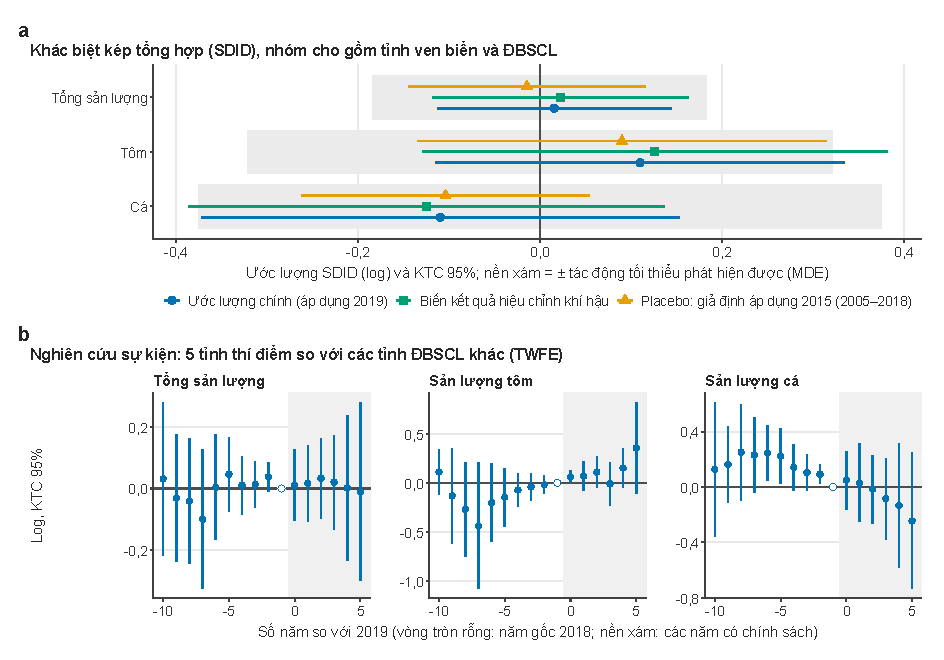
\includegraphics[width=138mm]{jv06_programme_effects.pdf}
    \caption{Tác động của chương trình lên sản lượng nuôi trồng cấp tỉnh. (a) Ước lượng khác biệt kép tổng hợp (SDID) \parencite{arkhangelsky2021} với đơn vị cho là các tỉnh ven biển và ĐBSCL khác (29 tỉnh cho tổng sản lượng và cá, 23 tỉnh cho tôm): ước lượng chính (áp dụng 2019), biến kết quả hiệu chỉnh khí hậu và placebo giả định áp dụng 2015 trên dữ liệu 2005--2018; KTC 95\%. Nền xám: $\pm$ tác động tối thiểu phát hiện được (MDE, bằng 2,8 lần sai số chuẩn placebo). (b) Hệ số nghiên cứu sự kiện với hiệu ứng cố định hai chiều, năm tỉnh thí điểm so với tám tỉnh ĐBSCL còn lại (với tôm: bốn tỉnh có sản lượng tôm bình quân trước 2019 từ 1.000 tấn trở lên), năm gốc 2018 (vòng tròn rỗng); KTC 95\% với sai số cụm theo tỉnh; nền xám: các năm có chính sách. Thang dọc ở (b) khác nhau giữa các biến kết quả.\\
    \textit{Nguồn:} Cục Thống kê; tính toán của tác giả.}
    \label{fig:sdid}
\end{figure}

\subsection{Hiểm họa và sản lượng hộ}

Ở cấp hộ, hiểm họa không dự báo được sản lượng (phương trình~\eqref{eq:hh}, Bảng~\ref{tab:hhfe}): không hệ số rủi ro nào có ý nghĩa với hiệu ứng cố định xã và tỉnh $\times$ năm, dù dùng sự kiện xã báo cáo, chỉ số năm hay chỉ số theo mùa. Kết quả bằng 0 có độ chính xác vừa phải: sai số chuẩn 0,05--0,10 trên mỗi độ lệch chuẩn, nên KTC 95\% vẫn chứa tác động âm 10--25\%. Ngoại lệ duy nhất là mưa cực trị tháng 7--12 với tôm ($-0{,}226$; SE 0,106; $p=0{,}033$) khi dùng hiệu ứng cố định vùng $\times$ năm; hệ số có dấu đúng dự đoán nhưng giảm còn $-0{,}079$ (SE 0,137) với hiệu ứng cố định tỉnh $\times$ năm. Trong 47 hệ số rủi ro đã ước lượng trên các biến kết quả, mẫu và cấu trúc hiệu ứng cố định, đây là giá trị $p$ duy nhất dưới 0,05. Sau hiệu chỉnh Holm \parencite{holm1979}, giá trị $p$ nhỏ nhất là 1,00; sau hiệu chỉnh Benjamini--Hochberg \parencite{benjamini1995}, giá trị $q$ nhỏ nhất là 0,91, nên hệ số này phù hợp với ngẫu nhiên. Hình~\ref{fig:hh} trình bày các hệ số chính và phân phối của toàn bộ 47 giá trị $p$, nằm trên hoặc dưới đường kỳ vọng khi không hiểm họa nào có tác động.

\textit{Diễn giải.} Có hai cách đọc một kết quả bằng 0, và chúng dẫn đến hàm ý khác nhau. Về độ chính xác, với sai số chuẩn của các hệ số chính từ 0,05 đến 0,106, khoảng tin cậy 95\% (hệ số $\pm 1{,}96\times$SE) rộng khoảng $\pm 0{,}10$ đến $\pm 0{,}21$ đơn vị asinh, xấp xỉ $\pm 10$--$21\%$ giá trị sản lượng cho mỗi độ lệch chuẩn của hiểm họa. Dữ liệu vì vậy loại trừ được tác động lớn, nhưng không loại trừ được tác động trung bình vài phần trăm, vốn đủ quan trọng với một hộ có biên lợi nhuận mỏng. Về tính đa dạng của các phép thử, với 47 hệ số và nếu không có tác động nào, số hệ số kỳ vọng có $p<0{,}05$ là $47\times 0{,}05\approx 2{,}35$; quan sát được một, nghĩa là không có dư thừa so với ngẫu nhiên. Cũng cần ghi nhận điều ước lượng này \emph{không} cho biết: hiệu ứng cố định tỉnh $\times$ năm hấp thụ 71\% và 68\% biến thiên của hai chỉ số (mục dữ liệu), nên phần hiểm họa còn lại để nhận dạng là phần chênh giữa các xã trong cùng tỉnh, đúng phần mà chỉ số lưới đo kém nhất (xem mục tiếp theo). Kết quả hộ và kết quả AUC vì thế cùng một thông điệp: chỉ số khí tượng lưới ở độ phân giải hiện có không bám sát tổn thất tại chỗ, nên rủi ro cơ sở của sản phẩm chỉ số thời tiết sẽ lớn.

Bốn cách giải thích tương thích với các kết quả bằng 0 này, mỗi cách gợi ý một bước tiếp theo: chỉ số bỏ sót rủi ro quan trọng (độ mặn, dịch bệnh, sốc nhiệt ngắn ngày); VHLSS che vụ mất trắng vì chỉ ghi sản lượng đã thu hoạch; hiệu ứng cố định tỉnh $\times$ năm hấp thụ phần lớn biến thiên hiểm họa; và khí hậu 2002--2008 chỉ có ở cấp tỉnh. Hàm ý chính sách trực tiếp: sản phẩm chỉ số thời tiết chỉ dựa trên mưa, nhiệt mà NĐ 346 cho phép sẽ có rủi ro cơ sở lớn với hộ nuôi tôm \parencite{jensen2016,clarke2016}.

\begin{figure}[!tbp]
\centering
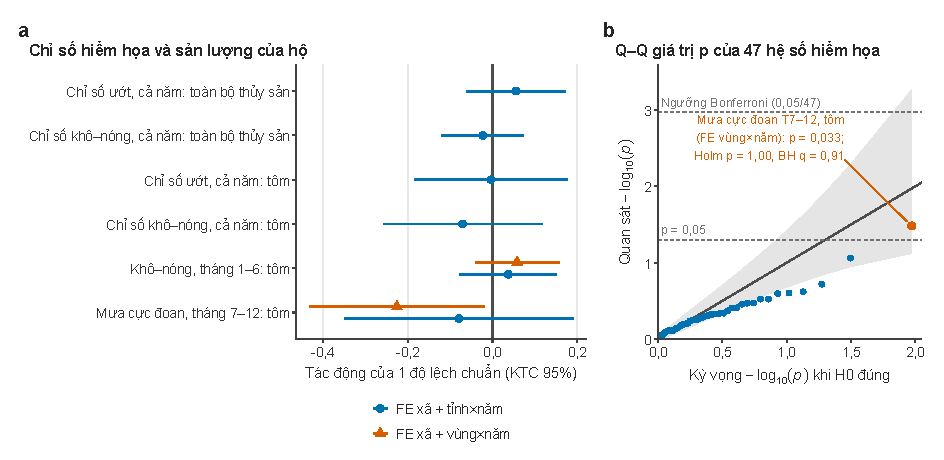
\includegraphics[width=125mm]{jv07_household_hazards.pdf}
\caption{Chỉ số hiểm họa và sản lượng nuôi trồng của hộ. (a) Tác động của mức tăng một độ lệch chuẩn ở từng chỉ số lên arcsinh của giá trị sản lượng, với hiệu ứng cố định xã và tỉnh $\times$ năm hoặc vùng $\times$ năm; sai số cụm theo xã; KTC 95\%. (b) Biểu đồ Q--Q của giá trị $p$ của 47 hệ số hiểm họa ước lượng trên các biến kết quả, mẫu và cấu trúc hiệu ứng cố định, so với phân phối đều kỳ vọng khi không có tác động; dải xám: khoảng 95\% theo từng điểm từ thống kê thứ tự. Giá trị hiệu chỉnh theo \textcite{holm1979} và \textcite{benjamini1995}. \textit{Nguồn:} VHLSS 2002--2024; CHIRPS; NASA POWER; IBTrACS; tính toán của tác giả.}
\label{fig:hh}
\end{figure}

\begin{table}[!tbp]
\centering\footnotesize
\caption{Hiểm họa khí hậu và sản lượng thủy sản của hộ (VHLSS, hiệu ứng cố định)}
\label{tab:hhfe}
\begin{tabular}{@{}llrrr@{}}
\toprule
Biến kết quả; hiệu ứng cố định & Biến rủi ro & Hệ số & SE & $N$ \\
\midrule
Sản lượng nuôi trồng; xã + tỉnh$\times$năm & Lũ (xã báo cáo) & $-0{,}066$ & 0,099 & 6.994 \\
 & Hạn (xã báo cáo) & $-0{,}042$ & 0,152 & \\
 & Dịch bệnh vật nuôi (xã báo cáo) & $-0{,}062$ & 0,071 & \\
Sản lượng nuôi trồng; xã + tỉnh$\times$năm & $H^{wet}$ & 0,055 & 0,059 & 10.442 \\
 & $H^{dry}$ & $-0{,}023$ & 0,050 & \\
\quad chỉ ĐBSCL & $H^{wet}$ & $-0{,}031$ & 0,092 & 6.748 \\
 & $H^{dry}$ & $-0{,}016$ & 0,070 & \\
Sản lượng tôm; xã + tỉnh$\times$năm & $H^{wet}$ & $-0{,}004$ & 0,092 & 3.637 \\
 & $H^{dry}$ & $-0{,}071$ & 0,096 & \\
Tôm, theo mùa; xã + vùng$\times$năm & $H^{dry}_D$ (khớp mùa) & 0,058 & 0,051 & 3.447 \\
 & $H^{wet}_W$ (khớp mùa) & $-0{,}226$ & 0,106 & \\
 & $H^{dry}_W$ (placebo) & $-0{,}032$ & 0,109 & \\
 & $H^{wet}_D$ (placebo) & 0,048 & 0,067 & \\
\quad cùng mô hình; xã + tỉnh$\times$năm & $H^{wet}_W$ & $-0{,}079$ & 0,137 & 3.413 \\
Cứu trợ (4D-107); xã + tỉnh$\times$năm & $H^{wet}$ & 0,007 & 0,014 & 7.517 \\
 & $H^{dry}$ & $-0{,}000$ & 0,008 & \\
Ngừng nuôi (hộ panel); tỉnh + năm & $H^{wet}$ & $-0{,}030$ & 0,038 & 1.200 \\
 & $H^{dry}$ & 0,031 & 0,052 & \\
\bottomrule
\end{tabular}
\begin{minipage}{\textwidth}\footnotesize
\textit{Ghi chú:} Sản lượng đo bằng asinh(giá trị, triệu đồng). Chỉ số chuẩn hóa, đo trong 12 tháng trước phỏng vấn. Ngừng nuôi: hộ nuôi ở vòng trước nhưng không nuôi ở vòng này (2004, 2006, 2008, 2014; 26,7\% ngừng). Kiểm soát: tuổi, giới, học vấn chủ hộ, quy mô hộ, tỷ lệ phụ thuộc. Sai số cụm theo xã. \textit{Nguồn:} VHLSS 2002--2024; CHIRPS; NASA POWER; IBTrACS; tính toán của tác giả.
\end{minipage}
\end{table}



\subsection{Chỉ số lưới có nhận diện được thiên tai tại chỗ?}

Sản phẩm chỉ số chi trả khi một biến đo lường vượt ngưỡng, nên giá trị của nó phụ thuộc vào mức độ chi trả bám theo các sự kiện gây tổn thất \parencite{clarke2016,jensen2016}. Phiếu xã VHLSS cho phép kiểm tra trực tiếp: ở mỗi vòng, cán bộ xã cho biết trong 12 tháng trước có lũ lụt, bão hay hạn hán hay không. Với 4.782 lượt xã ở các tỉnh ven biển và ĐBSCL (2004--2024), nghiên cứu này tính diện tích dưới đường cong ROC (AUC; \cite{hanley1982}) của từng chỉ số lưới đối với sự kiện tương ứng do xã báo cáo, theo hai cách: gộp và trong cùng tỉnh-năm. Cách thứ hai chỉ dùng các vòng có khí hậu cấp huyện (2010--2024) và hỏi chỉ số có xác định được \emph{xã nào} bị ảnh hưởng trong cùng một tỉnh, một năm hay không, đúng điều mà cơ chế kích hoạt dưới cấp tỉnh phải làm được. Khoảng tin cậy lấy từ 499 lần bootstrap theo xã.

\begin{figure}[!tbp]
\centering
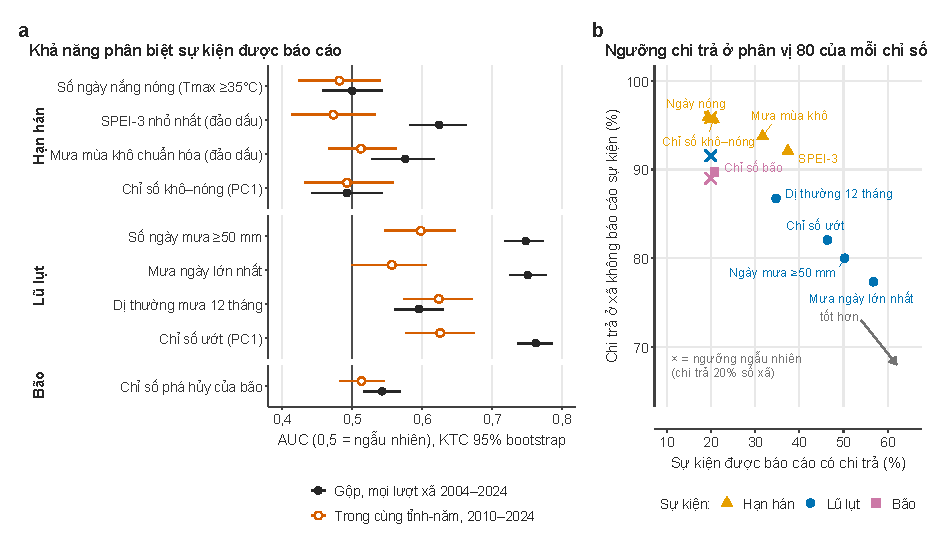
\includegraphics[width=148mm]{jv08_basis_risk.pdf}
\caption{Rủi ro cơ sở: chỉ số lưới có nhận diện được thiên tai mà cán bộ xã báo cáo? (a) Diện tích dưới đường ROC (AUC) và KTC 95\% bootstrap (499 lần, lấy mẫu lại theo xã). Gộp: mọi lượt xã 2004--2024. Trong cùng tỉnh-năm: chỉ số trừ trung bình tỉnh-năm, các vòng có khí hậu cấp huyện 2010--2024. 0,5 = không tốt hơn ngẫu nhiên. (b) Hiệu quả của ngưỡng chi trả khi chỉ số vượt phân vị 80: tỷ lệ sự kiện được báo cáo có chi trả so với tỷ lệ chi trả rơi vào xã không báo sự kiện đó; dấu $\times$ là giá trị kỳ vọng của ngưỡng ngẫu nhiên chi trả cho 20\% số xã. \textit{Nguồn:} phiếu xã VHLSS; CHIRPS; NASA POWER; IBTrACS; tính toán của tác giả.}
\label{fig:auc}
\end{figure}

\begin{table}[!tbp]
\centering\scriptsize
\setlength{\tabcolsep}{2.6pt}
\caption{Chỉ số lưới và thiên tai do xã báo cáo: khả năng phân biệt và hiệu quả của ngưỡng kích hoạt}
\label{tab:auc}
\begin{tabular}{@{}llrrccrr@{}}
\toprule
Thiên tai & Chỉ số & $N$ & Số xã báo & AUC gộp & AUC trong tỉnh-năm & Trúng & Chi trả sai \\
\midrule
Hạn hán & Số ngày Tmax $\geq$35°C & 3.728 & 157 & 0,50 [0,43; 0,58] & 0,48 [0,41; 0,56] & 0,19 & 0,96 \\
 & SPEI-3 nhỏ nhất (đảo dấu) & 3.727 & 157 & 0,62 [0,54; 0,70] & 0,47 [0,42; 0,55] & 0,37 & 0,92 \\
 & Mưa mùa khô (đảo dấu) & 4.782 & 190 & 0,58 [0,48; 0,67] & 0,51 [0,46; 0,58] & 0,32 & 0,94 \\
 & Chỉ số khô--nóng (PC1) & 3.727 & 157 & 0,49 [0,40; 0,58] & 0,49 [0,43; 0,56] & 0,21 & 0,96 \\
\midrule
Lũ lụt & Số ngày mưa $\geq$50 mm & 4.782 & 405 & 0,75 [0,70; 0,79] & 0,60 [0,53; 0,67] & 0,50 & 0,80 \\
 & Mưa ngày lớn nhất & 4.782 & 405 & 0,75 [0,70; 0,80] & 0,56 [0,50; 0,62] & 0,57 & 0,77 \\
 & Dị thường mưa 12 tháng & 4.782 & 405 & 0,60 [0,51; 0,68] & 0,62 [0,56; 0,68] & 0,35 & 0,87 \\
 & Chỉ số mưa--lũ (PC1) & 4.782 & 405 & 0,76 [0,73; 0,80] & 0,63 [0,57; 0,68] & 0,46 & 0,82 \\
\midrule
Bão & Chỉ số phá hủy của bão & 4.782 & 526 & 0,54 [0,49; 0,60] & 0,51 [0,48; 0,55] & 0,21 & 0,90 \\
\bottomrule
\end{tabular}
\begin{minipage}{\textwidth}\footnotesize
\textit{Ghi chú:} Đơn vị: lượt xã, các tỉnh ven biển và ĐBSCL, 2004--2024 (các vòng có phiếu xã). AUC trong tỉnh-năm: chỉ số trừ trung bình tỉnh-năm, các vòng 2010--2024. KTC 95\% từ 500 lần bootstrap theo cụm tỉnh-năm (Phụ lục G). Tỷ lệ trúng: tỷ lệ xã báo cáo sự kiện mà ngưỡng kích hoạt ở phân vị 80 của chỉ số sẽ chi trả (ngưỡng ngẫu nhiên chi trả 0,20). Chi trả sai: tỷ lệ lượt xã được kích hoạt nhưng không báo cáo sự kiện đó. \textit{Nguồn:} VHLSS; CHIRPS; NASA POWER; IBTrACS; tính toán của tác giả.
\end{minipage}
\end{table}

Khi gộp, chỉ số mưa phân biệt khá tốt xã bị lũ với xã không bị lũ (Hình~\ref{fig:auc}, Bảng~\ref{tab:auc}) (AUC 0,75--0,76 với số ngày mưa lớn, mưa ngày lớn nhất và chỉ số mưa--lũ), nhưng phần lớn khả năng này đến từ việc phân biệt tỉnh và năm mưa nhiều; trong cùng tỉnh-năm, AUC giảm còn 0,56--0,63. Hạn hán hầu như không được nhận diện: chỉ số tốt nhất là SPEI-3 nhỏ nhất có AUC gộp 0,62 và AUC trong tỉnh-năm 0,47; chỉ số nắng nóng và khô--nóng không tốt hơn ngẫu nhiên ở cả hai cách. Chỉ số bão gần như không phân biệt được xã báo có bão (0,54). Một ngưỡng kích hoạt đặt ở phân vị 80 của chỉ số, tức chi trả cho một trong năm lượt xã, sẽ chi trả ở 19--37\% số xã báo hạn, gần mức 20\% của ngưỡng ngẫu nhiên, và ở 35--57\% số xã báo lũ; từ 77\% đến 96\% số lần chi trả rơi vào xã không báo sự kiện đó. Báo cáo của xã cũng có sai số và ghi nhận sự kiện chứ không phải tổn thất của hộ, nên các con số này giúp khoanh vùng chứ không đo chính xác rủi ro cơ sở. Chúng củng cố kết quả cấp hộ: ở độ phân giải hiện có, chỉ số khí tượng lưới không bắt được các thiên tai tại chỗ mà chính quyền ghi nhận, nhất là hạn hán.

\textit{Diễn giải.} AUC là xác suất một xã có báo sự kiện có chỉ số cao hơn một xã không báo; 0,5 là ngẫu nhiên. Để đọc theo ngôn ngữ của người thiết kế sản phẩm, Hình~\ref{fig:lift} chuyển bảng thành hai đại lượng: tỷ số trúng so với ngưỡng ngẫu nhiên (tỷ lệ trúng chia cho 0,20) và tỷ lệ chi trả sai. Chỉ số tốt nhất cho lũ (mưa ngày lớn nhất) chi trả cho 57\% số xã báo lũ, gấp 2,9 lần ngưỡng ngẫu nhiên, nhưng vẫn có 77\% lượt chi trả rơi vào xã không báo lũ. Với hạn hán, tỷ số trúng chỉ từ 0,95 đến 1,85 lần và 92--96\% lượt chi trả là sai; với bão là 1,05 lần. Hàm ý định lượng là mọi sản phẩm chỉ số dùng chỉ số lưới sẽ chi trả cho hộ không tổn thất và bỏ sót hộ tổn thất ở tỷ lệ rất cao, và rủi ro cơ sở này không thể bù bằng cách nâng trợ cấp phí.

\begin{figure}[!tbp]
\centering
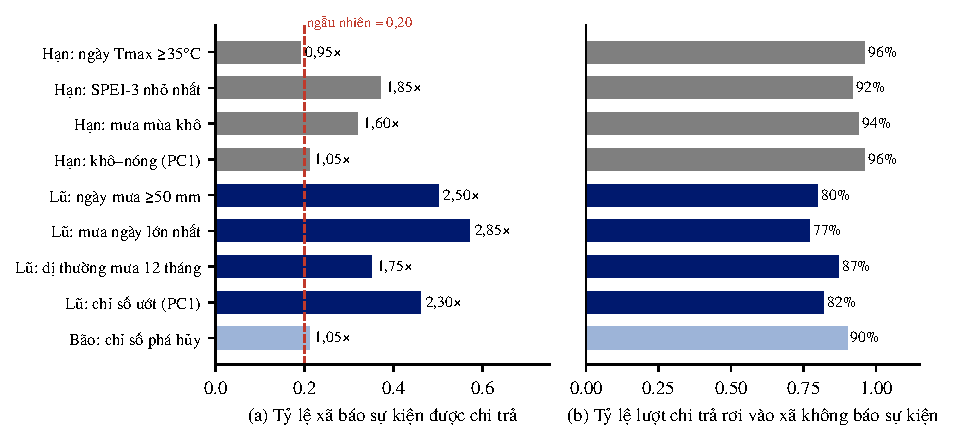
\includegraphics[width=140mm]{jv14_trigger_lift.pdf}
\caption{Hiệu quả ngưỡng kích hoạt ở phân vị 80 của từng chỉ số lưới. (a) Tỷ lệ xã báo sự kiện được chi trả; đường đứt: ngưỡng ngẫu nhiên chi trả cho 20\% số xã; số ghi cạnh thanh là tỷ số so với ngưỡng ngẫu nhiên. (b) Tỷ lệ lượt chi trả rơi vào xã không báo sự kiện. Xám: hạn hán; xanh đậm: lũ lụt; xanh nhạt: bão. \textit{Nguồn:} phiếu xã VHLSS; CHIRPS; NASA POWER; IBTrACS; giá trị lấy từ Bảng~\ref{tab:auc}; tính toán của tác giả.}
\label{fig:lift}
\end{figure}

\subsection{Định phí}

Phí thuần thô của sản phẩm chỉ số sản lượng tỉnh dao động 0--6,6\%, nhưng phần lớn biến thiên đó là nhiễu mẫu (Bảng~\ref{tab:premium}): với 20 quan sát mỗi tỉnh, hệ số tin cậy Bühlmann--Straub là 0,59 ở ĐBSCL ($k=13{,}7$) và 0,29 ở ven biển khác ($k=48{,}8$). Phí thô bằng 0 hoặc rất thấp của Bạc Liêu, Cà Mau phản ánh số liệu tổng tỉnh đã được làm trơn chứ không phải rủi ro ao nuôi thấp: sản lượng Bạc Liêu tăng liên tục mọi năm 2005--2024. Đuôi GPD gộp có $\hat\xi = 0{,}016$ với KTC bootstrap 95\% $[-0{,}47;\ 0{,}27]$, nên dữ liệu không phân biệt được đuôi mỏng hay dày; phụ phí đuôi phải dựa vào chuỗi hiểm họa dài kết hợp hàm thiệt hại, không dựa vào chuỗi sản lượng ngắn. Hình~\ref{fig:prem} cho thấy trọng số tin cậy kéo phí của từng tỉnh về gần trung bình vùng đến mức nào.

\textit{Diễn giải.} Hệ số tin cậy $Z=0{,}59$ nghĩa là phí của một tỉnh ĐBSCL dựa 59\% vào lịch sử của chính nó và 41\% vào trung bình vùng; ở ven biển khác $Z=0{,}29$, nên phí phần lớn là trung bình vùng. Hệ quả có thể kiểm tra trong Bảng~\ref{tab:premium}: phí của Vĩnh Long, tỉnh cao nhất, giảm từ 6,55\% xuống 4,48\% (giảm khoảng 32\%), còn phí của Bạc Liêu tăng từ 0 lên 0,59\%. Trong năm tỉnh thí điểm, phí theo độ tin cậy dao động từ 0,59\% đến 1,36\%, tức tỉnh cao nhất gấp 2,3 lần tỉnh thấp nhất, và chỉ Sóc Trăng và Bến Tre cao hơn phí đồng nhất 1,11\%. Điều này hạn chế cơ sở thực nghiệm cho phí khác nhau mạnh giữa các tỉnh thí điểm: chênh lệch phần lớn phản ánh nhiễu mẫu của chuỗi 20 năm. Cần nhắc rằng phí này đo thiếu hụt sản lượng tổng (gồm dịch bệnh và giá), không phải phí bảo hiểm thiên tai, và là sản phẩm chỉ số cấp tỉnh khác với sản phẩm bồi thường theo ao mô phỏng ở mục sau (phí gộp 3--5\% giá trị bảo hiểm); hai con số không so sánh trực tiếp được.

\begin{figure}[!tbp]
\centering
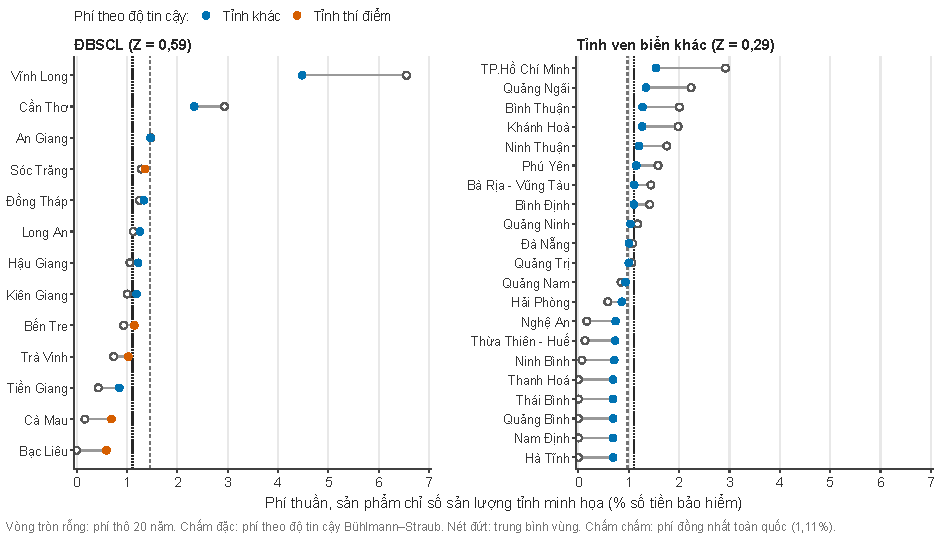
\includegraphics[width=142mm]{jv09_premium_credibility.pdf}
\caption{Phí thuần thô và phí theo độ tin cậy của sản phẩm chỉ số sản lượng tỉnh minh họa, 34 tỉnh ven biển và ĐBSCL. Vòng tròn rỗng: phí thô từ 20 năm thiếu hụt sản lượng (chi trả $=\max(0;\,0{,}9-Q/\hat Q)$ với xu thế bậc hai bỏ-một). Chấm đặc: phí theo độ tin cậy Bühlmann--Straub \parencite{buhlmann2005}, với hệ số tin cậy $Z=0{,}59$ (ĐBSCL) và $0{,}29$ (ven biển khác). Nét đứt: trung bình vùng; nét chấm: phí đồng nhất gia quyền theo sản lượng (1,11\%). Thiếu hụt sản lượng gồm cả tác động của dịch bệnh và giá, nên đây không phải biểu phí bảo hiểm thiên tai. \textit{Nguồn:} Cục Thống kê; tính toán của tác giả.}
\label{fig:prem}
\end{figure}

\begin{table}[!tbp]
\centering\footnotesize
\caption{Phí chỉ số sản lượng tỉnh minh họa: thô, có phụ phí đuôi và theo độ tin cậy (\% giá trị bảo hiểm)}
\label{tab:premium}
\begin{tabular}{@{}lcccccc@{}}
\toprule
Tỉnh & PPR thô & Năm chi trả & CVaR$_{95}$ & Có phụ phí & PPR tin cậy & Tin cậy + phụ phí \\
\midrule
Bạc Liêu & 0,00 & 0/20 & 0,0 & 0,00 & 0,59 & 0,59 \\
Bến Tre & 0,94 & 2/20 & 13,7 & 2,21 & 1,15 & 2,42 \\
Cà Mau & 0,16 & 1/20 & 3,3 & 0,48 & 0,69 & 1,00 \\
Sóc Trăng & 1,29 & 4/20 & 17,7 & 2,93 & 1,36 & 3,00 \\
Trà Vinh & 0,74 & 2/20 & 9,7 & 1,63 & 1,03 & 1,92 \\
\midrule
Vĩnh Long (cao nhất) & 6,55 & 8/20 & 48,7 & 10,76 & 4,48 & 8,69 \\
\midrule
Phí đồng nhất (34 tỉnh) & 1,11 & & & 2,10 & & \\
\bottomrule
\end{tabular}
\begin{minipage}{\textwidth}\footnotesize
\textit{Ghi chú:} Chi trả $=\max(0;\ 0{,}9-Q/\hat Q)$. Phụ phí $=0{,}10\times(\mathrm{CVaR}_{95}-\mathrm{PPR})$. Thiếu hụt sản lượng gồm cả dịch bệnh và giá, nên đây không phải biểu phí bảo hiểm thiên tai. \textit{Nguồn:} Cục Thống kê; tính toán của tác giả.
\end{minipage}
\end{table}

\subsection{Mô phỏng các thiết kế}

Mô phỏng cân bằng thị trường (Hình~\ref{fig:model}) cho phép so sánh trực tiếp ba phương án. Các phương án so sánh gồm khung hiện hành (hỗ trợ 90\%/20\%, phí chung), PA1 (khung NĐ 346 với 90\%/50\%, phí chung) và PA2 (PA1 cộng phí theo vùng rủi ro).

\begin{figure}[!tbp]
\centering
\resizebox{\textwidth}{!}{%
\begin{tikzpicture}[x=1cm, y=1cm, font=\footnotesize,
  bx/.style={draw=fblue!70, fill=paleblue, rounded corners=2pt, align=left, inner sep=5pt, text width=4.3cm, minimum height=3.5cm, anchor=center},
  pol/.style={draw=fgold!90!black, fill=palegold, rounded corners=2pt, align=left, inner sep=5pt, text width=15.0cm, anchor=center},
  outb/.style={draw=teal, fill=teal!12, rounded corners=2pt, align=left, inner sep=5pt, text width=15.0cm, anchor=center},
  ar/.style={-{Stealth[length=4pt]}, line width=0.8pt, color=fblue!75}]
\node[pol] (p) at (7.75,0) {\textbf{Biến chính sách (đổi giữa các phương án).} Mức hỗ trợ $s$ (90/20\% theo NĐ 58 hoặc 90/50\% theo NĐ 346) và cách chia ô $z$ (một ô chung, hoặc tỉnh $\times$ 5 bậc rủi ro theo bản đồ có độ chính xác $\rho$).};
\node[bx] (in) at (2.25,-3.2) {\textbf{1. Đầu vào}\\6.000 hộ ở 34 tỉnh, 300 năm. Tổn thất $L_{it}$ gồm phần chung của tỉnh (hụt sản lượng thật 2005--2024) và sự cố riêng của ao (xác suất $p_i$, chỉ hộ biết).};
\node[bx] (hh) at (7.75,-3.2) {\textbf{2. Hộ nuôi (cầu)}\\Mua nếu $\EV u(c^{\text{mua}})>\EV u(c^{\text{không mua}})$ với $u(c)=c^{1-\gamma}/(1-\gamma)$. Trả $(1-s)\pi_z$; nhận $\max(L_{it}-10\%,0)$.};
\node[bx] (dn) at (13.25,-3.2) {\textbf{3. Doanh nghiệp (cung)}\\Chỉ biết hộ ở ô $z$. Phí $\pi_z=(1+\lambda)\times$ bồi thường kỳ vọng của \emph{những hộ đang mua} trong ô $z$ (hòa vốn).};
\node[outb] (o) at (7.75,-8.3) {\textbf{4. Đầu ra.} Tỷ lệ tham gia; tổng chi hỗ trợ $\sum s\,\pi_z$; chỉ số lựa chọn ngược; bồi thường/phí (bình quân và năm xấu 1/20).};
\draw[ar] (in.east) -- (hh.west);
\draw[ar] (hh.east) -- (dn.west);
\draw[ar, color=fgold!90!black] (hh.north |- p.south) -- (hh.north);
\draw[ar, color=fgold!90!black] (dn.north |- p.south) -- (dn.north);
\draw[ar, dashed] ([xshift=-1.2cm]dn.south) -- ++(0,-0.7) -| ([xshift=1.2cm]hh.south);
\node[align=center, text width=5.2cm, font=\footnotesize\itshape, anchor=north] at (10.6,-5.75) {phí mới $\rightarrow$ hộ quyết định lại; lặp đến khi phí và nhóm người mua không đổi (cân bằng)};
\draw[ar] ([xshift=1.2cm]dn.south) -- ([xshift=1.2cm]dn.south |- o.north);
\end{tikzpicture}}
\caption{Cấu trúc mô hình mô phỏng thị trường bảo hiểm tôm. \textit{Nguồn:} tác giả; tham số là giả định.}
\label{fig:model}
\end{figure}

Kết quả so sánh các thiết kế theo tỷ lệ tham gia, chỉ số lựa chọn ngược và trợ cấp mỗi hộ (Bảng~\ref{tab:sim}, Hình~\ref{fig:scen}). Chỉ số lựa chọn ngược là tỷ số giữa tổn thất kỳ vọng của người mua và tổn thất kỳ vọng của toàn bộ hộ, bằng 1 khi không có lựa chọn ngược (Phương trình~\eqref{eq:premium} và lập luận ở mục khung lý thuyết); tham số của mô phỏng liệt kê ở Bảng~\ref{tab:simpar} trong Phụ lục. Vì tham số là giả định, kết quả cho biết thứ hạng chứ không cho biết mức độ. Định phí theo tỉnh gần như không giảm lựa chọn ngược: tỷ lệ tham gia của hộ không nghèo chỉ tăng từ 40,8\% lên 41,3\%. Định phí theo ô với bản đồ tương quan 0,8 với rủi ro thật nâng tỷ lệ này lên 54,1\% với chi trợ cấp/hộ thấp hơn. Nâng trợ cấp cho hộ không nghèo từ 20\% lên 50\% theo khung NĐ 346 nâng tỷ lệ của nhóm này lên 65,0\% nhưng tăng chi trợ cấp/hộ 40\% và không xử lý lựa chọn ngược; kết hợp hai công cụ cho độ phủ cao nhất (81,1\%).

\textit{Diễn giải hiệu quả chi phí.} Đọc cùng nhau hai cột tỷ lệ tham gia chung và trợ cấp mỗi hộ (đều lấy từ Bảng~\ref{tab:sim}), có ba kết luận. (i) Nâng trợ cấp hộ không nghèo từ 20\% lên 50\% với phí chung tăng độ phủ chung 17,3 điểm (56,3\% lên 73,6\%) nhưng tăng trợ cấp mỗi hộ từ 0,96\% lên 1,35\% của cải, tức khoảng 0,023 điểm của cải cho mỗi điểm phần trăm độ phủ thêm. (ii) Giữ nguyên trợ cấp 20\% nhưng phí theo ô với $\rho=0{,}8$ tăng độ phủ 10,4 điểm và \emph{giảm} trợ cấp mỗi hộ xuống 0,91\%, vì trợ cấp là một tỷ lệ của phí và phí ở các ô rủi ro thấp thấp hơn phí chung. (iii) Thêm phí theo ô lên trên khung 50\% tăng độ phủ thêm 12,3 điểm (73,6\% lên 85,9\%) chỉ tốn thêm 0,02 điểm của cải trợ cấp. Thứ hạng này là điều kiện của giả định (Bảng~\ref{tab:simpar}): nó phụ thuộc vào việc bản đồ có độ chính xác $\rho$ đủ cao, và với $\rho=0{,}5$ lợi ích còn rất nhỏ (Hình~\ref{fig:sens}). Cột $\sum\Delta CE$/trợ cấp nằm trong khoảng 1,11--1,18, nghĩa là theo mô hình mỗi đồng trợ cấp tạo ra giá trị phúc lợi (tương đương chắc chắn) hơi lớn hơn một đồng; con số giảm nhẹ khi trợ cấp tăng (1,13 xuống 1,11) và tăng khi thông tin tốt hơn (1,18 khi thông tin đầy đủ), cùng chiều với lập luận rằng cải thiện thông tin là bổ sung cho trợ cấp.

\begin{table}[!tbp]
\centering\footnotesize
\caption{Cân bằng thị trường mô phỏng theo cấu trúc thông tin và mức trợ cấp (tham số giả định)}
\label{tab:sim}
\begin{tabular}{@{}lcccccc@{}}
\toprule
Thiết kế & \multicolumn{3}{c}{Tỷ lệ tham gia (\%)} & Chỉ số & Trợ cấp/hộ & $\sum\Delta CE$/ \\
\cmidrule(lr){2-4}
 & Chung & Nghèo & Khác & lựa chọn ngược & (\% của cải) & trợ cấp \\
\midrule
\multicolumn{7}{@{}l}{\textit{A. Trợ cấp hiện hành 90\%/20\%}} \\
Phí đồng nhất & 56,3 & 93,3 & 40,8 & 1,39 & 0,96 & 1,13 \\
Phí theo tỉnh & 56,9 & 93,9 & 41,3 & 1,37 & 0,95 & 1,13 \\
Phí theo ô, $\rho=0{,}5$ & 60,8 & 95,5 & 46,3 & 1,31 & 0,93 & 1,14 \\
Phí theo ô, $\rho=0{,}8$ & 66,7 & 97,0 & 54,1 & 1,23 & 0,91 & 1,15 \\
Phí theo ô, $\rho=0{,}95$ & 73,9 & 98,1 & 63,7 & 1,16 & 0,88 & 1,17 \\
Thông tin đầy đủ & 99,2 & 99,2 & 99,2 & 1,01 & 0,90 & 1,18 \\
\midrule
\multicolumn{7}{@{}l}{\textit{B. Trợ cấp 90\%/50\% (khung NĐ 346/2026)}} \\
Phí đồng nhất & 73,6 & 94,0 & 65,0 & 1,25 & 1,35 & 1,11 \\
Phí theo ô, $\rho=0{,}8$ & 85,9 & 97,2 & 81,1 & 1,12 & 1,37 & 1,12 \\
\bottomrule
\end{tabular}
\begin{minipage}{\textwidth}\footnotesize
\textit{Ghi chú:} 6.000 hộ phân bổ vào 34 tỉnh theo sản lượng 2024; xác suất tổn thất riêng Beta(1,2; 8), mức thiệt hại Beta(2; 5); khấu trừ 10\%; CRRA $\gamma\sim U(1;3)$; phụ phí 25\%; 30\% hộ nghèo; chưa có cứu trợ, cơ chế kích hoạt và dịch bệnh. \textit{Nguồn:} mô phỏng của tác giả.
\end{minipage}
\end{table}

\begin{figure}[!tbp]
\centering
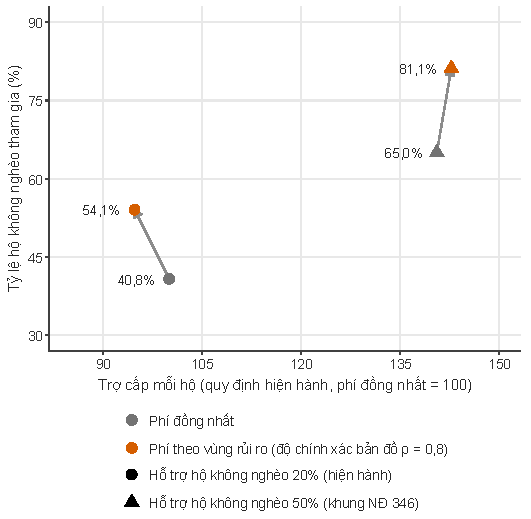
\includegraphics[width=90mm]{jv10_policy_scenarios.pdf}
\caption{Tỷ lệ tham gia mô phỏng của hộ không nghèo và chi trợ cấp mỗi hộ theo bốn thiết kế; mũi tên: chuyển từ phí đồng nhất sang phí theo vùng rủi ro ở mỗi mức trợ cấp. Chi trợ cấp lấy quy định hiện hành với phí đồng nhất làm gốc (= 100). Mọi tham số đều là giả định (xem Bảng~\ref{tab:sim}); hình xếp hạng các thiết kế, không dự báo tỷ lệ tham gia. \textit{Nguồn:} mô phỏng của tác giả.}
\label{fig:scen}
\end{figure}

Phí theo vùng tác động qua hai kênh tách biệt (Hình~\ref{fig:sim}, Bảng~\ref{tab:mech}). Ở khung 90/50\% với phí chung (PA1), nhóm hộ không nghèo có rủi ro thật thấp nhất phải trả phí 4,7\% giá trị bảo hiểm, gấp khoảng 5,6 lần tổn thất kỳ vọng của nhóm (0,84\%), nên chỉ 6,8\% trong nhóm mua; với phí theo vùng (PA2) phí nhóm này giảm còn 2,7\% và tỷ lệ mua lên 33,4\%. Nhóm rủi ro cao nhất mua gần như toàn bộ ở cả hai phương án (100\%), nên lợi ích của phí theo vùng đến từ việc giữ được nhóm rủi ro thấp trong thị trường, và đây là cơ chế lựa chọn ngược trong mô hình.

\begin{figure}[!tbp]
\centering
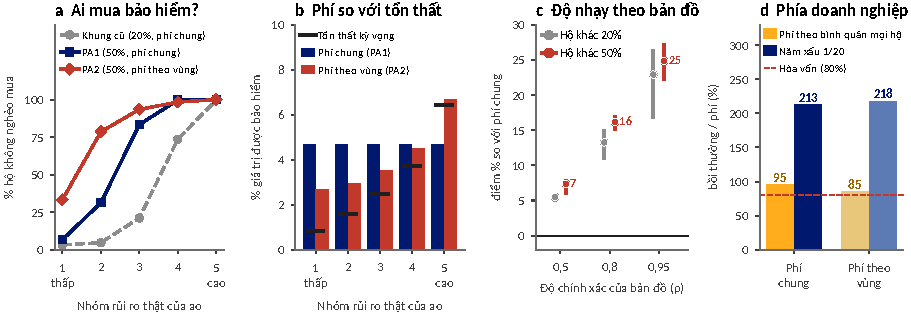
\includegraphics[width=\textwidth]{pb_v4_results.pdf}
\caption{Kết quả mô phỏng. (a), (b) Hộ không nghèo chia thành 5 nhóm bằng nhau theo rủi ro thật của ao: tỷ lệ mua và phí so với tổn thất kỳ vọng. (c) Mức tăng độ phủ của phí theo vùng so với phí chung theo độ chính xác bản đồ $\rho$; thanh dọc: phụ phí quản lý 15--40\%. (d) Tỷ lệ bồi thường/phí của doanh nghiệp ở mức hỗ trợ 50\%.\\
\textit{Nguồn:} mô phỏng của tác giả, tham số giả định (Bảng~\ref{tab:sim}).}
\label{fig:sim}
\end{figure}

\begin{table}[!tbp]
\centering\footnotesize
\caption{Cơ chế: tỷ lệ mua và phí theo nhóm rủi ro thật của hộ không nghèo (mô phỏng, tham số giả định)}
\label{tab:mech}
\begin{tabular}{@{}lccccc@{}}
\toprule
 & \multicolumn{5}{c}{Nhóm rủi ro thật của ao (1 = thấp nhất)} \\
\cmidrule(lr){2-6}
 & 1 & 2 & 3 & 4 & 5 \\
\midrule
Tổn thất kỳ vọng (\% giá trị bảo hiểm) & 0,84 & 1,58 & 2,49 & 3,74 & 6,45 \\
\midrule
\multicolumn{6}{@{}l}{\textit{Tỷ lệ mua (\%)}} \\
Khung hiện hành (hỗ trợ 20\%, phí chung) & 3,3 & 4,7 & 21,2 & 73,6 & 99,8 \\
PA1 (hỗ trợ 50\%, phí chung) & 6,8 & 31,3 & 83,4 & 99,6 & 100,0 \\
PA2 (hỗ trợ 50\%, phí theo vùng) & 33,4 & 78,6 & 93,5 & 98,4 & 100,0 \\
\midrule
\multicolumn{6}{@{}l}{\textit{Phí gộp (\% giá trị bảo hiểm)}} \\
Khung hiện hành (phí chung) & 5,23 & 5,23 & 5,23 & 5,23 & 5,23 \\
PA1 (phí chung) & 4,69 & 4,69 & 4,69 & 4,69 & 4,69 \\
PA2 (phí theo vùng) & 2,69 & 2,93 & 3,52 & 4,51 & 6,69 \\
\bottomrule
\end{tabular}
\begin{minipage}{\textwidth}\footnotesize
\textit{Ghi chú:} $\rho=0{,}8$ cho PA2. Phí chung của PA1 (4,69\%) thấp hơn khung hiện hành (5,23\%); phí là điểm cân bằng nên đổi theo thành phần người mua khi hỗ trợ tăng. \textit{Nguồn:} mô phỏng của tác giả.
\end{minipage}
\end{table}

Độ nhạy: trong 18 kết hợp của $\rho\in\{0{,}5;\,0{,}8;\,0{,}95\}$, phụ phí quản lý và mức hỗ trợ cho hộ khác (20\% hoặc 50\%), phí theo vùng luôn tăng độ phủ so với phí chung, từ 4,9 đến 27,3 điểm phần trăm; với bản đồ kém ($\rho=0{,}5$) chỉ còn 4,9--7,9 điểm. Dịch hệ số ngại rủi ro $\gamma$ lên hoặc xuống không đổi thứ hạng (mức tăng 14,0--16,9 điểm với hỗ trợ 50\%). Hình~\ref{fig:sens} cho thấy dạng của kết quả này: lợi ích của phí theo vùng lớn hơn khi phụ phí thấp và bản đồ chính xác. Với hộ không nghèo ở mức hỗ trợ 20\%, chuyển sang phí theo ô tăng tỷ lệ tham gia 26,4 điểm khi $\rho=0{,}95$ và phụ phí 15\%, nhưng chỉ 4,9 điểm khi $\rho=0{,}5$ và phụ phí 40\%. Hai điều kiện này, độ chính xác bản đồ và chi phí vận hành, chính là các điều kiện chính sách có thể tác động; bảng đầy đủ ở Phụ lục (Bảng~\ref{tab:sens}). Bồi thường/phí bình quân của doanh nghiệp hòa vốn ở 80\% theo xây dựng, nhưng trong năm xấu 1/20 vẫn khoảng 2,1--2,2 lần phí (phân vị 95), nên phần đuôi vẫn cần tái bảo hiểm.

\begin{figure}[!tbp]
\centering
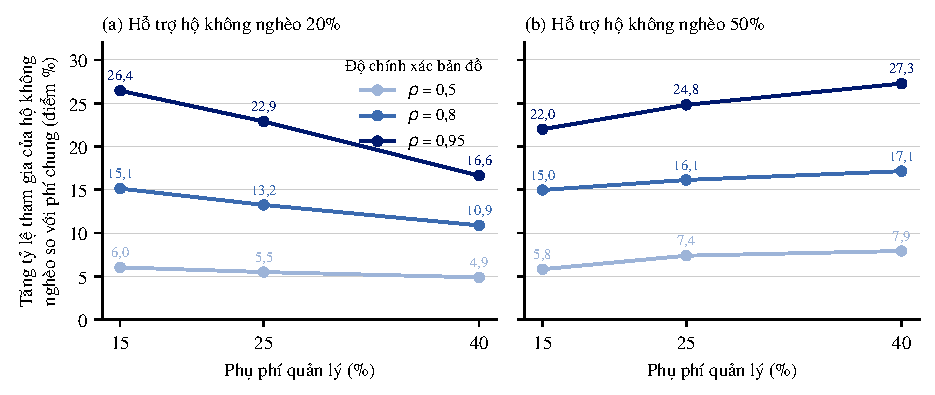
\includegraphics[width=135mm]{jv13_sensitivity.pdf}
\caption{Độ nhạy của lợi ích phí theo vùng: mức tăng tỷ lệ tham gia của hộ không nghèo (điểm phần trăm) khi chuyển từ phí chung sang phí theo ô, theo phụ phí quản lý (15\%, 25\%, 40\%) và độ chính xác bản đồ $\rho$. (a) Hỗ trợ hộ không nghèo 20\%; (b) 50\%. Hộ nghèo luôn hỗ trợ 90\%. Mọi tham số là giả định. \textit{Nguồn:} mô phỏng của tác giả.}
\label{fig:sens}
\end{figure}

Khoảng cách giữa mô phỏng và quan sát là hàm ý quan trọng nhất của bước một: mô phỏng dự báo tỷ lệ tham gia khoảng 56\% với khung hiện hành, trong khi tỷ lệ quan sát gần bằng 0. Khoảng cách này gợi ý rằng các ràng buộc chưa có trong mô hình (cơ chế kích hoạt bằng công bố, loại trừ dịch bệnh, doanh nghiệp không chào bán) chi phối mạnh hơn lựa chọn ngược; mô hình không kiểm định điều đó. Vì vậy, kết quả mô phỏng nên được đọc như thứ hạng các thiết kế định phí với điều kiện sản phẩm được chào bán, không phải dự báo tỷ lệ tham gia.

\subsection{Kiểm định độ vững}
\label{sec:robust}

Kết luận không có tác động chỉ có giá trị khi nó không đổi khi đổi đặc tả (độ nhạy) và khi suy luận với mẫu nhỏ được xử lý đúng (suy luận). Phần lớn kết quả chính là ước lượng gần bằng không với khoảng tin cậy rộng, nên hai chiều này cần được kiểm tra riêng. Bảng~\ref{tab:robustplan} liệt kê bốn nhóm kiểm định, rủi ro nhận dạng mà mỗi nhóm nhắm tới và điều nó \emph{không} chứng minh được (chi tiết số liệu ở Phụ lục G).

\begin{table}[!tbp]
\centering\footnotesize
\caption{Kế hoạch kiểm định độ vững}
\label{tab:robustplan}
\begin{tabularx}{\textwidth}{@{}>{\raggedright\arraybackslash}p{2.6cm}>{\raggedright\arraybackslash}X>{\raggedright\arraybackslash}X@{}}
\toprule
Nhóm & Kiểm định & Rủi ro nhận dạng được xử lý \\
\midrule
A. Panel tỉnh (bão $\to$ sản lượng) & Bỏ lần lượt từng tỉnh; hoán vị phơi nhiễm trong tỉnh (5.000 lần); thêm độ trễ $t-2$; xu thế tuyến tính riêng từng tỉnh; biến nhị phân gió $\geq$34 kt; bỏ tỉnh ngoài ĐBSCL; bỏ tỉnh tôm nhỏ; bỏ 2020--2021 & Một tỉnh chi phối hệ số; suy luận với 32--34 cụm; xu thế riêng tương quan với phơi nhiễm \\
B. Đánh giá chương trình & DiD với xu thế riêng, bỏ 2011--2013, thời điểm sau 2020; placebo thời gian 2010--2017; suy luận ngẫu nhiên hóa trên $\binom{13}{5}=1.287$ cách gán; SDID bỏ từng đơn vị đối chứng, đổi năm bắt đầu, tập đối chứng rộng & Xu thế song song, số cụm rất ít (5 tỉnh thí điểm), đối chứng chi phối \\
C. Hộ gia đình & Đường cong đặc tả 144 hệ số (kết quả $\times$ chỉ số $\times$ mẫu $\times$ hiệu ứng cố định $\times$ biến kiểm soát); cụm theo xã, huyện, tỉnh; hoán vị trong tỉnh-năm (2.000 lần); winsor 1--99 và bỏ 1\% cao nhất; kiểm định tương đương TOST & Tự do chọn đặc tả, phụ thuộc không gian, ngoại lai, và phân biệt ``không có hiệu ứng'' với ``không đủ lực'' \\
D. Chỉ số lưới (AUC) & Bootstrap theo cụm tỉnh-năm (500 lần) thay cho bootstrap theo xã; hoán vị nhãn sự kiện trong năm (1.000 lần); AUC riêng ĐBSCL; tỷ số trúng ở phân vị 70, 80, 90 & Phụ thuộc không gian làm KTC hẹp giả; ngưỡng kích hoạt chọn tùy ý \\
\bottomrule
\end{tabularx}
\begin{minipage}{\textwidth}\footnotesize
\textit{Ghi chú:} Kiểm định tương đương dùng biên $\delta = 0{,}20$ (đơn vị asinh của giá trị sản lượng trên một độ lệch chuẩn hiểm họa), là lựa chọn của tác giả, không phải ngưỡng có cơ sở kinh tế đã được xác lập. \textit{Nguồn:} tác giả.
\end{minipage}
\end{table}

Chạy lại hồi quy panel tỉnh trên bộ dữ liệu đóng gói bằng chính mã của Bảng~\ref{tab:twfe} cho hệ số tôm cùng năm là $-0{,}359$ (SE cụm 0,560), không phải $-0{,}531$ như Bảng~\ref{tab:twfe}; hệ số tổng sản lượng ($-0{,}161$ so với $-0{,}159$), DiD tổng sản lượng (0,005), hệ số hộ $H^{wet}$ (0,055; SE 0,059) và SDID tập đối chứng rộng (0,016; SE 0,066) thì khớp. Số quan sát và số tỉnh khớp (579 và 32), nên chênh lệch nằm ở giá trị biến phơi nhiễm hoặc sản lượng tôm của bản dữ liệu đã dùng cho Bảng~\ref{tab:twfe}; chưa xác định được nguyên nhân. Mọi số trong mục này vì thế là ước lượng \emph{của cùng mã trên bộ dữ liệu đóng gói}, và Bảng~\ref{tab:twfe} giữ nguyên số đã công bố cho đến khi đối chiếu xong. Kết luận định tính (không có ý nghĩa thống kê ở đặc tả cơ sở, dấu âm) không phụ thuộc vào chênh lệch này. Số quan sát của hồi quy hộ là 11.191, so với 10.442 ở Bảng~\ref{tab:hhfe}, trong khi hệ số và SE khớp. Ước lượng điểm SDID khớp Bảng~\ref{tab:did} nhưng SE của cài đặt R (0,110) hơi lớn hơn SE của Python (0,101); và phần SDID tôm dưới đây dùng 4 tỉnh đối chứng có sản lượng tôm đủ lớn, ít hơn tập đối chứng của Bảng~\ref{tab:did}.

\subsubsection*{A. Panel tỉnh: bão và sản lượng}

Dấu âm của hệ số bão--tôm không phụ thuộc vào một tỉnh cụ thể, nhưng ý nghĩa thống kê thì có: cả 32 lần bỏ một tỉnh đều cho hệ số âm, và lần nào cũng không có ý nghĩa 5\% (Hình~\ref{fig:robA}a). Hệ số dao động từ $-0{,}773$ (bỏ Đà Nẵng) đến $-0{,}045$ (bỏ Khánh Hòa); không phép bỏ nào đưa $|t|$ vượt 1,96, và hệ số độ trễ $t-1$ ($-1{,}204$ đến $-0{,}233$) chỉ có ý nghĩa ở một phép bỏ. Dấu âm bền nhưng độ lớn thay đổi gấp 17 lần, tức kết quả chịu ảnh hưởng của vài tỉnh ngoài ĐBSCL có bão mạnh. Suy luận hoán vị (Hình~\ref{fig:robA}b) cho giá trị $p$ gần với $p$ của sai số cụm CR1 với hệ số cùng năm (0,510 so với 0,514) và tổng sản lượng (0,603 so với 0,612); với hệ số trễ, hoán vị cho $p$ thấp hơn (0,207 so với 0,314 của CR1). Vì $p$ của CR1 không thấp hơn $p$ hoán vị trong cả ba trường hợp, mức không có ý nghĩa ở đặc tả cơ sở không phải do sai số cụm với 32 cụm đánh giá thấp độ bất định.

\begin{figure}[!tbp]
\centering
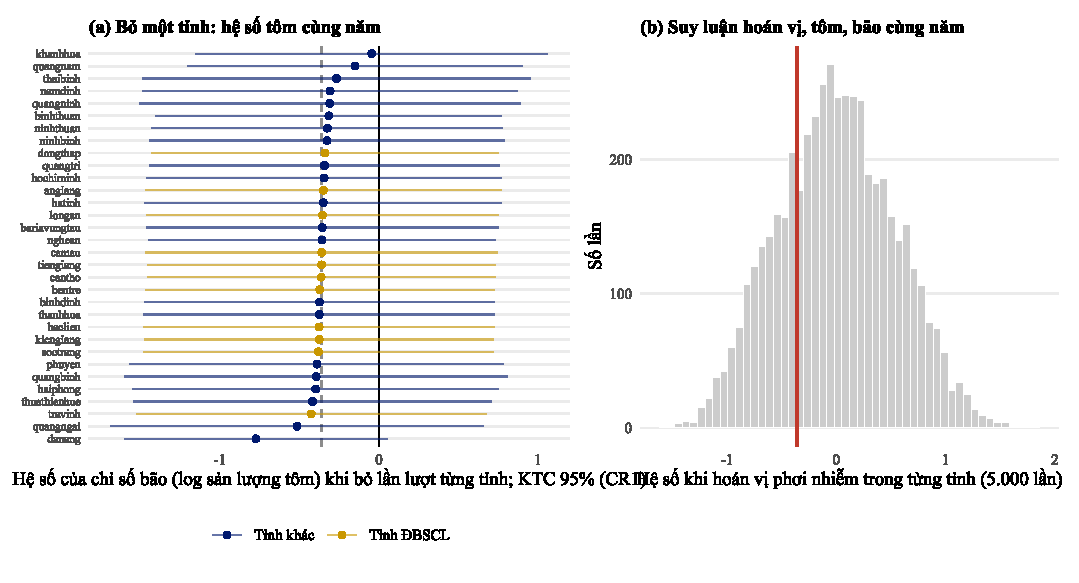
\includegraphics[width=\textwidth]{RA_province_robust.pdf}
\caption{Độ vững của hệ số bão--sản lượng tôm ở cấp tỉnh. (a) Hệ số năm $t$ khi bỏ lần lượt từng tỉnh (điểm) và KTC 95\% theo sai số cụm CR1; đường đứt: ước lượng cơ sở, đường đặc: 0. (b) Phân phối hệ số khi hoán vị phơi nhiễm trong từng tỉnh qua các năm (5.000 lần); đường đỏ: ước lượng quan sát.}
\label{fig:robA}
\begin{minipage}{\textwidth}\footnotesize
\textit{Nguồn:} tính toán của tác giả từ dữ liệu bảng cấp tỉnh và chỉ số bão (Phụ lục F).
\end{minipage}
\end{figure}

Ba đặc tả thay thế cho thấy hệ số tôm nhạy với xu thế và cách xây dựng mẫu. Thêm xu thế tuyến tính riêng từng tỉnh làm hệ số tôm đổi thành $-0{,}586$ (SE 0,286; $p=0{,}049$) và hệ số trễ thành $-0{,}908$ ($p=0{,}019$). Bỏ tỉnh có sản lượng tôm trung bình dưới 1.000 tấn cho $-0{,}774$ ($p=0{,}083$) và $-1{,}339$ cho độ trễ ($p=0{,}016$). Biến nhị phân (có gió $\geq$34 kt) cho $-0{,}025$ (SE 0,052), và tác động tích lũy $t$ cộng $t-1$ là $-1{,}053$ (SE 1,241). Nghiên cứu này đọc kết quả này theo ba tầng. Thứ nhất, dấu luôn âm và độ lớn kinh tế không nhỏ (một cơn bão chuẩn gắn với sản lượng tôm thấp hơn 0,36 đến 1,34 log tùy đặc tả), nên nghiên cứu này không thể tuyên bố rằng bão không ảnh hưởng đến tôm. Thứ hai, ý nghĩa thống kê phụ thuộc đặc tả: có khi xu thế riêng hấp thụ biến thiên chậm của sản lượng, phần dư của phơi nhiễm hẹp lại và sai số giảm một nửa; đây là kết quả nhạy với đặc tả chứ không phải bằng chứng mới. Thứ ba, hệ số vẫn được nhận dạng gần như hoàn toàn từ ngoài ĐBSCL (bỏ các tỉnh ĐBSCL chỉ đổi $-0{,}359$ thành $-0{,}505$), nên dù đúng nhân quả nó không cho biết gì về ĐBSCL, vì ĐBSCL hầu như không có bão. Đây là điểm quan trọng nhất của nhóm A và củng cố lập luận ở Mục~\ref{sec:discussion} rằng bằng chứng bão--sản lượng không thể ngoại suy sang vùng bảo hiểm.

\subsubsection*{B. Đánh giá chương trình: DiD, placebo và suy luận ngẫu nhiên hóa}

Với tổng sản lượng, kết luận không đổi: ước lượng DiD gần 0 ở mọi biến thể: 0,005 (SE 0,090) cơ sở, 0,047 (SE 0,163) khi thêm xu thế riêng, $-0{,}009$ khi bỏ 2011--2013 và 0,005 khi coi 2020 là năm bắt đầu. Suy luận ngẫu nhiên hóa trên cả 1.287 cách chọn 5 trong 13 tỉnh cho $p=0{,}957$, tức không thể phân biệt với ngẫu nhiên. Placebo thời gian (Hình~\ref{fig:robB}a) và suy luận ngẫu nhiên hóa (Hình~\ref{fig:robB}b) cho tổng sản lượng đều trong khoảng $-0{,}039$ đến 0,023 với KTC chứa 0 ở cả tám năm giả định 2010--2017. SDID cho $-0{,}040$ (SE 0,110 theo cài đặt R); khi bỏ lần lượt từng tỉnh đối chứng ước lượng nằm trong $[-0{,}079;\,-0{,}018]$, đổi năm bắt đầu sang 2018 hoặc 2020 cho $-0{,}047$ và $-0{,}055$, và tập đối chứng rộng cho 0,016 (SE 0,066). Bốn kiểm định khác nhau về tổng sản lượng đều dẫn đến cùng một đọc: không có dấu hiệu tác động cấp tỉnh, và khoảng loại trừ phía trên khoảng 0,18 log.

Với tôm và cá, bức tranh kém rõ ràng hơn. (i) Tôm: DiD cơ sở 0,178 (SE 0,156) nhưng 0,381 (SE 0,182) khi thêm xu thế riêng, và placebo giả định 2010, 2011, 2012 cho $-0{,}257$, $-0{,}219$ và $-0{,}153$ với $|t|$ lớn hơn 2 (chỉ 9 cụm đối chứng và thí điểm nên $p$ chính xác kém tin cậy), trong khi các năm 2013--2017 gần 0. Placebo có ý nghĩa ở giai đoạn đầu cho thấy chuỗi tôm của nhóm thí điểm và 4 tỉnh đối chứng chưa song song ở giữa thập niên 2000, vì vậy ước lượng DiD của tôm không nên được đọc như tác động chương trình. SDID cho tôm với 4 đối chứng là 0,078 và không tính được sai số chuẩn ổn định với chỉ 4 tỉnh đối chứng; bỏ từng tỉnh đối chứng cho 0,034--0,123. (ii) Cá: DiD $-0{,}215$ (SE 0,085) với $p$ ngẫu nhiên hóa 0,049, âm ở mọi biến thể ($-0{,}145$ đến $-0{,}232$), nhưng SDID chỉ $-0{,}123$ (SE 0,146) và placebo trôi dần về $-0{,}120$ vào năm 2017, tức xu hướng giảm tương đối có từ trước năm bắt đầu và SDID, vốn gán trọng số để khớp xu thế trước, hấp thụ phần lớn. Cá tra mới vào chương trình năm 2022, nên một tác động tiêu cực thực sự của bảo hiểm lên sản lượng cá cũng khó giải thích về cơ chế. Nghiên cứu này coi nó là tín hiệu cần theo dõi ở chuỗi dài hơn, không phải phát hiện.

\begin{figure}[!tbp]
\centering
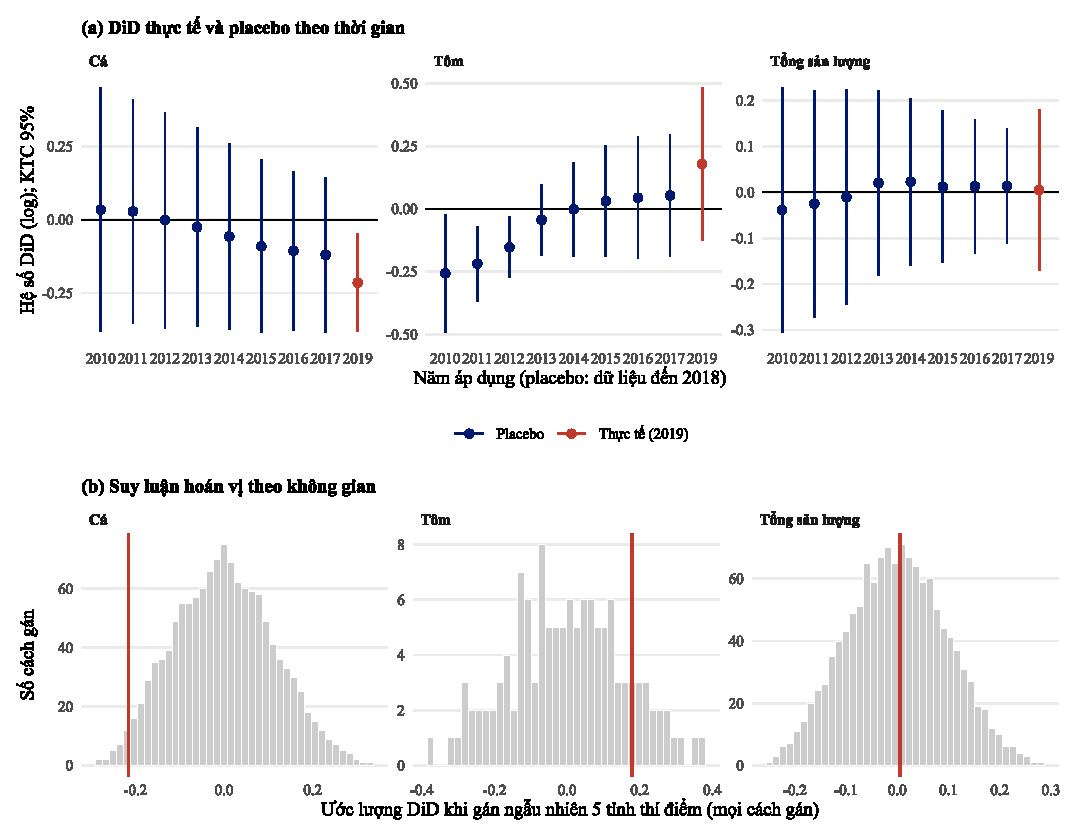
\includegraphics[width=\textwidth]{RB_policy_robust.pdf}
\caption{Độ vững của đánh giá chương trình. (a) Ước lượng DiD thực tế (năm 2019, đỏ) và placebo thời gian (năm giả định 2010--2017, chỉ dùng dữ liệu trước 2019, xanh) cho tổng sản lượng, tôm và cá; KTC 95\% theo sai số cụm. (b) Phân phối ước lượng DiD khi gán ngẫu nhiên 5 tỉnh thí điểm trong 13 tỉnh ĐBSCL (mọi cách gán); đường đỏ: ước lượng quan sát.}
\label{fig:robB}
\begin{minipage}{\textwidth}\footnotesize
\textit{Ghi chú:} Tôm chỉ có 4 tỉnh đối chứng nên các KTC không đáng tin ở mức tuyệt đối. \textit{Nguồn:} tính toán của tác giả (Phụ lục F).
\end{minipage}
\end{figure}

\subsubsection*{C. Hộ gia đình: đường cong đặc tả, cụm sai số, hoán vị và tương đương}

Kết quả hiểm họa mưa--lũ không phải sản phẩm của việc chọn đặc tả: trong 144 đặc tả chỉ 4 hệ số có $p<0{,}05$ (Hình~\ref{fig:robC}). Đường cong gồm 144 hệ số: ba biến kết quả (giá trị sản lượng nuôi trồng, của tôm, và tổng đầu ra của hộ có hoạt động thủy sản), hai cách đo hiểm họa (chuẩn hóa $z$ và PCA), hai mẫu (cả nước ven biển và ĐBSCL), ba bộ hiệu ứng cố định (tỉnh$\times$năm, vùng$\times$năm, năm) và có hay không biến kiểm soát. Trung vị là 0,013 và khoảng $[-0{,}168;\,0{,}126]$. Con số này (2,8\%) thấp hơn 7,2 hệ số kỳ vọng do ngẫu nhiên ở mức 5\%, và cả bốn là hệ số $H^{wet}$ (PCA) của tôm, âm ($-0{,}104$ đến $-0{,}168$), trên mẫu cả nước và với hiệu ứng cố định \emph{không} phải tỉnh$\times$năm; tức chỉ khi không hấp thụ biến thiên ở cấp tỉnh$\times$năm mới xuất hiện tín hiệu, đúng chỗ biến thiên đó bị nghi lẫn với cú sốc cấp tỉnh. Không hệ số $H^{dry}$ nào có ý nghĩa. Đọc chung: không có kết quả ``nổi lên'' chỉ vì chọn đặc tả có lợi, và bốn ngoại lệ có thể giải thích bằng nhiễu cấp tỉnh.

Nới cấp cụm hầu như không đổi kết luận (Bảng~\ref{tab:cluster}): với $H^{wet}$ của sản lượng nuôi trồng, SE là 0,059 (xã, 2.371 cụm), 0,064 (huyện, 549) và 0,074 (tỉnh, 31), $p$ từ 0,350 đến 0,461. Với tôm, $H^{dry}$ ở cụm tỉnh (29 cụm) cho $-0{,}071$ (SE 0,035; $p=0{,}052$); biên giới này nên được đọc là tín hiệu yếu, vì $p$ dựa trên $t$ với 28 bậc tự do và 29 cụm, chưa qua hiệu chỉnh đa kiểm định. Hoán vị $(H^{wet},H^{dry})$ giữa các xã trong cùng tỉnh-năm cho $p=0{,}210$ và 0,480 với sản lượng nuôi trồng, 0,946 và 0,204 với tôm, khớp với $p$ cụm theo xã. Winsor 1--99 hoặc bỏ 1\% cao nhất chỉ nâng $H^{wet}$ lên 0,058 và 0,081 ($p=0{,}153$).

Quan trọng hơn, kiểm định tương đương trả lời câu hỏi ``không hiệu ứng hay không đủ lực'' (Hình~\ref{fig:robCb}). Hệ số $H^{wet}$ của sản lượng nuôi trồng là 0,055 với KTC 95\% $[-0{,}061;\,0{,}172]$ nằm trong biên $\pm0{,}20$ ($p_{\text{TOST}}=0{,}007$), và độ hiệu lực tối thiểu phát hiện được ở lực 80\% là 0,166. Nói cách khác, hiệu ứng của mỗi độ lệch chuẩn hiểm họa mưa--lũ lớn hơn 0,20 đơn vị asinh đã bị loại trừ, và mẫu đủ lực phát hiện hiệu ứng cỡ 0,17; đây là bằng chứng cho một hiệu ứng nhỏ chứ không chỉ là mẫu thiếu lực. Với tôm, $H^{wet}$ cũng nằm trong biên ($p_{\text{TOST}}=0{,}017$) nhưng $H^{dry}$ thì không ($p_{\text{TOST}}=0{,}090$, MDE 0,270): mẫu 3.912 lượt hộ nuôi tôm chỉ loại được hiệu ứng khô--nóng lớn hơn khoảng 0,27 chứ không loại được hiệu ứng trung bình. Điều này thu hẹp nhận định ở Mục~\ref{sec:discussion}: ``chỉ số hiểm họa lưới không dự báo được sản lượng hộ'' vững với hiểm họa mưa--lũ, ít chắc chắn hơn với hạn và nhiệt ở hộ tôm.

\begin{figure}[!tbp]
\centering
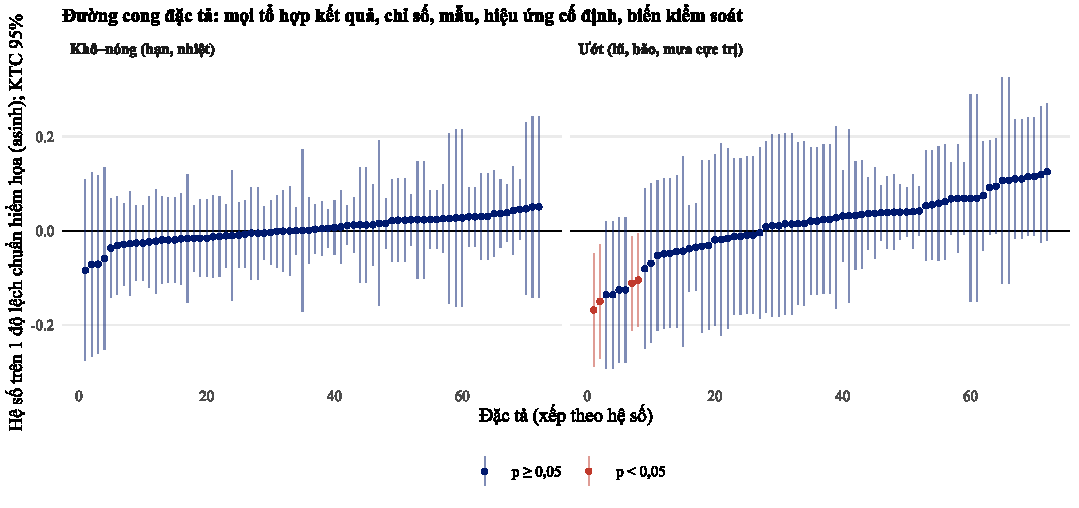
\includegraphics[width=\textwidth]{RC_spec_curve.pdf}
\caption{Đường cong đặc tả của hệ số hiểm họa--sản lượng hộ. Mỗi điểm là một hệ số trong 144 đặc tả (thanh: KTC 95\%), xếp theo độ lớn trong từng khối; đỏ: $p<0{,}05$, xanh: $p\geq0{,}05$. Panel trái: hệ số hiểm họa mưa--lũ; panel phải: hiểm họa khô--nóng.}
\label{fig:robC}
\begin{minipage}{\textwidth}\footnotesize
\textit{Nguồn:} tính toán của tác giả từ VHLSS (Phụ lục F).
\end{minipage}
\end{figure}

\begin{figure}[!tbp]
\centering
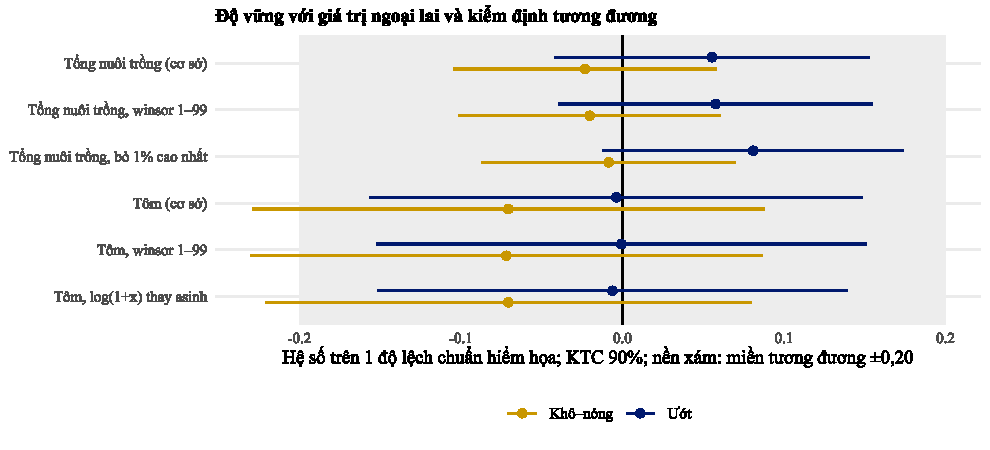
\includegraphics[width=0.92\textwidth]{RC_equivalence.pdf}
\caption{Kiểm định tương đương (TOST). Điểm: ước lượng; thanh: KTC 90\% (dùng cho TOST); vùng xám: biên tương đương $\pm0{,}20$. Một hệ số được coi là ``nhỏ'' khi toàn bộ KTC 90\% nằm trong biên.}
\label{fig:robCb}
\begin{minipage}{\textwidth}\footnotesize
\textit{Ghi chú:} Biên $\delta$ do tác giả chọn; kết luận tương đương chỉ đúng với biên đó. \textit{Nguồn:} tính toán của tác giả.
\end{minipage}
\end{figure}

\subsubsection*{D. Chỉ số lưới: độ vững của AUC}

Chỉ số lưới mưa--lũ phân biệt được ở mức vừa phải xã có lũ với xã không có lũ trong cùng tỉnh-năm, còn với hạn thì không; kết luận này không đổi khi bootstrap theo cụm tỉnh-năm, cụm bảo vệ trước phụ thuộc không gian giữa các xã cùng tỉnh-năm (Hình~\ref{fig:robD}). AUC gộp của chỉ số mưa--lũ PC1 là 0,763 (KTC 0,730--0,800), và AUC trong tỉnh-năm là 0,626 (0,571--0,677): khoảng sau tách khỏi 0,5 ở ba chỉ số: ngày mưa $\geq$50 mm (0,598; 0,532--0,665), dị thường mưa 12 tháng (0,624; 0,563--0,680) và PC1 mưa--lũ. Với mưa ngày lớn nhất, AUC trong tỉnh-năm là 0,557 (0,496--0,620), KTC chứa 0,5. Với hạn hán, bốn chỉ số đều cho AUC trong tỉnh-năm 0,47--0,51: ngày Tmax$\geq$35°C 0,48 (gộp 0,50), SPEI-3 nhỏ nhất 0,47 (KTC 0,42--0,55; gộp 0,62), mưa mùa khô 0,51 và PC1 khô--nóng 0,49. Như vậy ở hạn hán không có chỉ số nào nhận diện được xã bị hạn hơn một xã cùng tỉnh-năm; AUC gộp của SPEI-3 cao hơn chủ yếu nhờ khác biệt giữa các tỉnh. Hoán vị nhãn sự kiện trong từng năm cho $p<0{,}001$ với bốn chỉ số lũ và SPEI-3 ($p=0{,}001$) nhưng với hạn không có ý nghĩa: $p=0{,}884$ với ngày nóng, 0,242 với mưa mùa khô và 0,999 với PC1 khô--nóng.

AUC riêng ĐBSCL đảo thứ tự: chỉ số lũ thấp hơn (0,43--0,67) trong khi chỉ số hạn cao hơn (0,65--0,71), nhưng mẫu ĐBSCL nhỏ và chưa có KTC bootstrap cho phần này, nên chỉ ghi nhận như tín hiệu. Về ngưỡng kích hoạt, ở phân vị 70, 80, 90 chỉ số tốt nhất cho lũ (ngày mưa $\geq$50 mm) cho tỷ số trúng 2,45, 2,51 và 2,88 lần ngưỡng ngẫu nhiên, nhưng tỷ lệ chi trả sai vẫn 81\%, 80\% và 78\%: nâng ngưỡng lên 90 thì tỷ số trúng cải thiện nhưng chỉ còn 29\% số xã báo lũ được chi trả. Hạn hán có tỷ số trúng 0,77--1,88. Tức đánh đổi giữa bỏ sót và chi trả sai không thể giải bằng cách chọn lại ngưỡng.

\begin{figure}[!tbp]
\centering
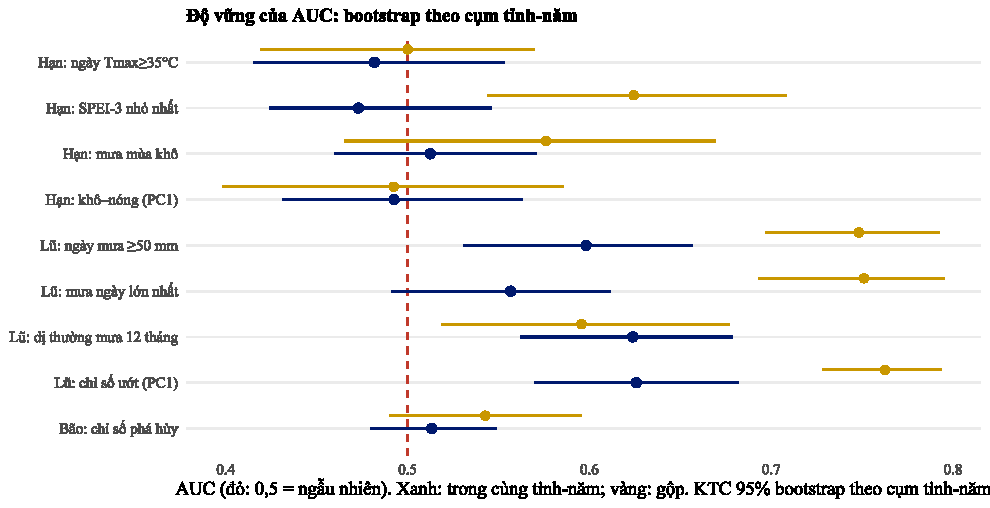
\includegraphics[width=0.92\textwidth]{RD_auc_cluster.pdf}
\caption{AUC của chỉ số lưới với thiên tai do xã báo cáo, với KTC 95\% bootstrap theo cụm tỉnh-năm (500 lần). Xanh: AUC trong tỉnh-năm; vàng: AUC gộp; đường đứt đỏ: 0,5 (ngẫu nhiên).}
\label{fig:robD}
\begin{minipage}{\textwidth}\footnotesize
\textit{Nguồn:} tính toán của tác giả từ phiếu xã VHLSS và dữ liệu lưới (Phụ lục F).
\end{minipage}
\end{figure}

\subsubsection*{Tổng hợp độ vững}

Bảng~\ref{tab:robustsum} tổng hợp kết quả theo từng phát hiện chính. Ba phát hiện vững: SDID tổng sản lượng xấp xỉ 0, hiểm họa mưa--lũ không dự báo sản lượng hộ (đủ lực phát hiện hiệu ứng cỡ 0,17 và loại trừ hiệu ứng ngoài $\pm0{,}20$), và chỉ số hạn không nhận diện được xã bị hạn. Chỉ số lũ nhận diện được xã bị lũ ở mức vừa phải, vì ba trong bốn chỉ số có KTC tách khỏi 0,5. Hai phát hiện không vững: dấu và ý nghĩa của hệ số bão--tôm (phụ thuộc đặc tả, nhận dạng từ ngoài vùng bảo hiểm) và kết quả theo từng loài của đánh giá chương trình (tôm có xu thế trước không song song, cá nhạy với xu thế).

\begin{table}[!tbp]
\centering\footnotesize
\caption{Tổng hợp độ vững của các phát hiện định lượng}
\label{tab:robustsum}
\begin{tabularx}{\textwidth}{@{}>{\raggedright\arraybackslash}p{3.7cm}>{\raggedright\arraybackslash}X>{\raggedright\arraybackslash}p{2.1cm}@{}}
\toprule
Phát hiện & Bằng chứng từ kiểm định & Đánh giá \\
\midrule
SDID tổng sản lượng $\approx 0$ & $-0{,}040$ (SE 0,110); bỏ từng đối chứng $[-0{,}079;-0{,}018]$; placebo 2010--2017 đều trong $\pm0{,}04$; $p$ ngẫu nhiên hóa 0,957 & Vững \\
Bão $\to$ tôm cấp tỉnh: dấu ổn định, ý nghĩa thì không & Dấu âm ở mọi đặc tả nhưng $p$ từ 0,016 đến 0,63 tùy đặc tả; nhận dạng từ ngoài ĐBSCL & Không vững; không dùng để ngoại suy \\
Tôm và cá của đánh giá chương trình & Placebo tôm 2010--2012 có ý nghĩa; cá nhạy với xu thế & Không vững; chỉ mang tính chỉ báo \\
$H^{wet}$ không dự báo sản lượng hộ & 4/144 hệ số có $p<0{,}05$; TOST trong $\pm0{,}20$; MDE 0,166; $p$ hoán vị 0,210 & Vững \\
$H^{dry}$ không dự báo sản lượng hộ tôm & TOST không loại được hiệu ứng ở biên 0,20 ($p=0{,}090$) & Yếu (thiếu lực) \\
AUC trong tỉnh-năm gần 0,5 với hạn & 0,47--0,51; KTC bootstrap cụm tỉnh-năm chứa 0,5 ở cả bốn chỉ số hạn & Vững \\
AUC trong tỉnh-năm với lũ 0,56--0,63 & KTC của ba trong bốn chỉ số lũ tách khỏi 0,5, riêng mưa ngày lớn nhất thì không & Vững ở mức vừa phải \\
\bottomrule
\end{tabularx}
\begin{minipage}{\textwidth}\footnotesize
\textit{Ghi chú:} Số liệu từ Bảng~\ref{tab:rA1}--\ref{tab:rD}. \textit{Nguồn:} tác giả.
\end{minipage}
\end{table}

%====================================================================
\section{Thảo luận}
\label{sec:discussion}

\subsection{Vì sao độ phủ gần bằng 0}

Bằng chứng cho phép một xếp hạng tạm thời các giải thích. \textit{Phía cung rút lui} được ủng hộ bởi kinh nghiệm 2011--2013 (bồi thường gấp khoảng 3,1 lần phí, tái bảo hiểm từ chối rủi ro tôm) và việc không tỉnh nuôi tôm nào nằm trong danh sách địa phương triển khai sau 2019. \textit{Thiết kế cơ chế kích hoạt và phạm vi} được ủng hộ bởi văn bản pháp lý: hiểm họa mãn tính như hạn mặn có trong danh mục nhưng hiếm khi được ``công bố'' ở quy mô ao nuôi, còn dịch bệnh, rủi ro hộ gặp nhiều nhất theo các khảo sát \parencite{kiet2021ruiro,joffre2018}, bị loại trừ. \textit{Rủi ro từ thiện} phù hợp với số liệu năm 2022, khi cứu trợ đến với 11\% hộ thí điểm còn bảo hiểm bằng 0, nhưng VHLSS không nhận dạng được hiệu ứng lấn át, và việc NĐ 02/2017 có khấu trừ bồi thường bảo hiểm khi tính hỗ trợ hay không còn cần đối chiếu. \textit{Lựa chọn ngược do phí đồng nhất} có cơ sở lý thuyết và là trọng tâm của phân tích định phí, nhưng tự nó không giải thích được độ phủ bằng 0: mô phỏng dự báo độ phủ khoảng 56\% với khung hiện hành, rất xa tỷ lệ quan sát. Các khảo sát mức sẵn lòng chi trả cho thấy có cầu tiềm năng khi sản phẩm phù hợp \parencite{nguyenkat2021,tu2025}, nên thiếu cầu thuần túy không phải lời giải thích chính. Bảng~\ref{tab:hyp} đối chiếu từng giả thuyết ở mục khung lý thuyết với bằng chứng.

\begin{table}[!tbp]
\centering\footnotesize
\caption{Giả thuyết và bằng chứng}
\label{tab:hyp}
\begin{tabularx}{\textwidth}{@{}l>{\raggedright\arraybackslash}p{3.7cm}>{\raggedright\arraybackslash}X>{\raggedright\arraybackslash}p{2.5cm}@{}}
\toprule
 & Nội dung & Bằng chứng chính & Kết luận \\
\midrule
H1 & Tổn thất khó dự báo bằng hiểm họa đo được & Hệ số hộ không có ý nghĩa sau Holm và BH (47 phép thử); AUC trong tỉnh-năm 0,47--0,51 với hạn, 0,56--0,63 với lũ & Ủng hộ cho hạn; ủng hộ vừa cho lũ. Chuẩn đối chiếu là báo cáo xã \\
H2 & Tham gia và chi trả không phản ứng, tác động lên sản lượng $\approx 0$ & Chi trả $\leq 1{,}1\%$ mọi vòng; SDID $\approx 0$, MDE 0,18 cho tổng sản lượng & Ủng hộ. Chỉ là ITT, không kết luận về hiệu quả của bảo hiểm \\
H3 & Khác biệt không gian đủ lớn để định phí theo ô & Moran's $I$ 0,76--0,81; 24--32\% biến thiên trong tỉnh; nhưng độ mặn, dịch bệnh chưa quan sát & Ủng hộ một phần: đúng với khí tượng, chưa kiểm định với hiểm họa chính của tôm \\
H4 & Trợ cấp lũy tiến cộng phí theo rủi ro hiệu quả hơn nâng trợ cấp cào bằng & Mô phỏng: phí theo ô ở mức 20\% cho thêm 10,4 điểm độ phủ với trợ cấp thấp hơn; nâng lên 50\% cho thêm 17,3 điểm với trợ cấp cao hơn 40\% & Ủng hộ có điều kiện: tham số giả định và $\rho$ phải đủ cao; chưa so sánh ngân sách tương đương \\
\bottomrule
\end{tabularx}
\begin{minipage}{\textwidth}\footnotesize
\textit{Nguồn:} tổng hợp của tác giả từ các Bảng~\ref{tab:firststage}--\ref{tab:sim}.
\end{minipage}
\end{table}

\subsection{So sánh với các nghiên cứu trước}

Mục này đối chiếu từng kết quả với các dòng nghiên cứu trước đây ở phần tổng quan, theo thứ tự: kết quả của nghiên cứu này phù hợp, phù hợp một phần, khác hay chưa kiểm định được so với kết luận của nghiên cứu trước đây, và vì sao.

\textit{Lựa chọn ngược và phân loại rủi ro.} Lý thuyết cho rằng phí đồng nhất đẩy hộ rủi ro thấp ra khỏi thị trường \parencite{akerlof1970,rothschild1976}, làm cân bằng có độ phủ thấp hơn mức hiệu quả \parencite{einav2011}, và phân loại theo đặc điểm quan sát được có thể cải thiện phúc lợi \parencite{crocker1986}. Mô phỏng của nghiên cứu này phù hợp với chiều này: ở khung 90/50\% với phí chung, nhóm hộ không nghèo rủi ro thấp nhất chỉ mua 6,8\% còn nhóm cao nhất mua 100\%, và phí theo vùng nâng tỷ lệ mua của nhóm thấp nhất lên 33,4\%. Tuy nhiên đây là kiểm chứng \emph{nội tại của mô hình} với tham số giả định, không phải kiểm định thực nghiệm; nghiên cứu này không có dữ liệu bồi thường để quan sát lựa chọn ngược thực sự, và kết quả chỉ nói rằng nếu lựa chọn ngược có mặt thì phí theo vùng giúp ích, không nói rằng nó là nguyên nhân của độ phủ bằng 0. Ở điểm này nghiên cứu này khác với các nghiên cứu ở nước thu nhập cao, nơi lựa chọn ngược có thể quan sát từ hợp đồng.

\textit{Rủi ro hiệp biến và đuôi.} Tổn thất thiên tai tương quan trong vùng nên chia sẻ phi chính thức không đủ \parencite{townsend1994,dercon2002} và doanh nghiệp cần vốn hay tái bảo hiểm cho đuôi \parencite{kunreuther1996}. Bằng chứng của nghiên cứu này phù hợp với điều này: bồi thường/phí của doanh nghiệp trong năm xấu 1/20 vẫn gấp khoảng 2,1--2,2 lần phí dù hòa vốn trung bình, đuôi GPD không phân biệt được đuôi mỏng hay dày, và kinh nghiệm thí điểm 2011--2013 (3,1 lần) cho thấy phần đuôi đã từng làm sụp đổ chương trình. Đây là bằng chứng nhất quán nhất của nghiên cứu này với nghiên cứu trước đây.

\textit{Rủi ro cơ sở và cầu thấp.} Nghiên cứu trước đây cho thấy rủi ro cơ sở lớn làm giảm cầu bảo hiểm chỉ số \parencite{gine2008,clarke2016,jensen2016}. Kết quả AUC của nghiên cứu này phù hợp về hướng nhưng khác về cách đo: các nghiên cứu trên đo rủi ro cơ sở so với năng suất hoặc tổn thất của hộ, còn nghiên cứu này đo so với thiên tai do xã báo cáo. Bằng chứng ở cấp xã ít khắt khe hơn (báo cáo xã không phải tổn thất hộ), nhưng kết quả vẫn xấu: tốt nhất cho lũ chi trả đúng 57\% số xã nhưng 77\% lượt chi trả là sai, và hạn hán gần như không phân biệt được với ngẫu nhiên. Vì chuẩn đối chiếu thiên về chấp nhận chỉ số, rủi ro cơ sở thực với hộ có thể còn lớn hơn. Cần phân biệt: khác với các thí nghiệm ở Ấn Độ hay Kenya, nơi cầu thấp là kết quả hành vi của hộ khi được chào bán, ở Việt Nam sản phẩm \emph{hầu như không được chào bán}, nên cầu thấp chưa thể quan sát.

\textit{Thanh khoản, niềm tin và mạng lưới xã hội.} \textcite{casaburi2018} và \textcite{cai2015} chỉ ra thanh khoản và niềm tin quyết định tham gia. Nghiên cứu này không kiểm định các cơ chế này vì VHLSS không ghi việc mua bảo hiểm. Tuy nhiên, kết quả ngược với hướng suy diễn rằng giải pháp chủ yếu là can thiệp phía cầu (giáo dục, trả phí lúc thu hoạch): nếu doanh nghiệp không chào bán hoặc hợp đồng không chi trả khi tổn thất xảy ra, cải thiện thanh khoản của hộ không tạo ra độ phủ. Đây là điểm khác biệt chính của bối cảnh nuôi tôm ở ĐBSCL so với nghiên cứu trước đây về bẫy cân bằng thấp \parencite{colexiong2017,carter2017}.

\textit{Rủi ro từ thiện.} Các nghiên cứu ở Hoa Kỳ và Đức cho thấy kỳ vọng cứu trợ làm giảm mua bảo hiểm \parencite{coate1995,kousky2018,andor2020}. Bằng chứng của nghiên cứu này chỉ nhất quán về hướng (cứu trợ đến 11\% hộ thí điểm năm 2022 khi bảo hiểm bằng 0), không nhận dạng được tác động nhân quả, và nghiên cứu này không tìm thấy ước lượng tương ứng cho bảo hiểm nông nghiệp trợ cấp ở nước đang phát triển, nên đây là chỗ trống nghiên cứu trước đây hơn là một phát hiện.

\textit{Rủi ro thủy sản và phạm vi hợp đồng.} Nghiên cứu ở Na Uy, Bangladesh và ĐBSCL xếp giá và dịch bệnh trên rủi ro thời tiết \parencite{bergfjord2009,ahsan2011,lecheong2010}. Việc hợp đồng Việt Nam loại trừ dịch bệnh phù hợp với kết luận rằng sản phẩm chỉ bảo vệ phần rủi ro ít quan trọng nhất với hộ. Nghiên cứu này không đo được tỷ trọng tổn thất theo nguyên nhân, nên không định lượng được phần bị loại trừ; đây là hạn chế dữ liệu, không phải bất đồng với nghiên cứu trước đây.

\textit{Trợ cấp và phân phối.} \textcite{binswanger2012} lập luận rằng hộ khá giả đã tự bảo hiểm còn hộ nghèo nhất không đủ tiền đóng phí; \textcite{goodwin2013} chỉ ra trợ cấp phí có thể lệch quyết định sản xuất. Mô phỏng của nghiên cứu này cho thấy hộ nghèo (hỗ trợ 90\%) mua 93--98\% ở mọi thiết kế trừ trường hợp thông tin đầy đủ (99,2\%), còn biến động độ phủ nằm ở hộ không nghèo (40,8\% đến 99,2\%); điều này gợi ý ràng buộc tiếp cận của hộ nghèo ít do giá, trong khi phân loại nghèo bằng VHLSS chỉ có đến 2020 và danh sách hộ nghèo địa phương có thể không trùng với hộ nuôi tôm. Nghiên cứu này không đánh giá được méo mó sản xuất do trợ cấp.

\textit{Biến đổi khí hậu và độ mặn.} Sóng nhiệt biển đang tăng toàn cầu \parencite{oliver2018,frolicher2018}, và độ mặn ở ĐBSCL tăng do hạ thấp lòng sông chứ không chỉ do nước biển dâng \parencite{eslami2019}. Kết quả của nghiên cứu này nhất quán với hướng thứ nhất: số ngày sóng nhiệt biển ở vùng ven biển các tỉnh thí điểm tăng từ 6,6 lên 53,2 ngày/năm. Việc không thấy xu thế nhiệt trên đất liền không mâu thuẫn với nghiên cứu trước đây về độ mặn, vì nghiên cứu này không quan sát độ mặn; thiếu số liệu này vừa là hạn chế vừa là ưu tiên dữ liệu.

\textit{Phương pháp.} Ước lượng hộ bằng 0 khác với kinh tế lượng khí hậu cấp quốc gia và tỉnh, vốn thường tìm thấy tác động của biến thiên khí hậu bên trong đơn vị \parencite{dell2014,hsiang2016}. Hai khác biệt giải thích: nghiên cứu này dùng hiệu ứng cố định tỉnh $\times$ năm, loại bỏ phần lớn biến thiên mà các nghiên cứu kia khai thác, và đơn vị quan sát là hộ nuôi với thu hoạch có thể điều chỉnh. Nghiên cứu này vì vậy đưa ra một kết quả bằng 0 \emph{có điều kiện}, không phải bác bỏ tác động của khí hậu lên ngành thủy sản.

\begingroup\footnotesize
\begin{longtable}{@{}>{\raggedright\arraybackslash}p{3.3cm}>{\raggedright\arraybackslash}p{8.2cm}>{\raggedright\arraybackslash}p{3.2cm}@{}}
\caption{Đối chiếu kết quả của nghiên cứu này với nghiên cứu trước}\label{tab:lit}\\
\toprule
Dòng nghiên cứu trước đây & Kết quả của nghiên cứu này so với nghiên cứu trước đây & Đánh giá \\
\midrule\endfirsthead
\toprule Dòng nghiên cứu trước đây & Kết quả của nghiên cứu này so với nghiên cứu trước đây & Đánh giá \\ \midrule\endhead
\bottomrule\endfoot
Lựa chọn ngược \parencite{rothschild1976,einav2011} & Cùng chiều trong mô phỏng (nhóm thấp nhất mua 6,8\% so với 100\%); chưa có kiểm định thực nghiệm & Phù hợp, chưa kiểm định \\
Rủi ro hiệp biến và đuôi \parencite{townsend1994,kunreuther1996} & Bồi thường/phí 2,1--2,2 lần ở năm xấu; thí điểm 3,1 lần & Phù hợp \\
Rủi ro cơ sở \parencite{clarke2016,jensen2016} & AUC 0,47--0,63 trong tỉnh-năm; 77--96\% chi trả sai; chuẩn đối chiếu là báo cáo xã & Phù hợp về hướng, đo khác \\
Thanh khoản, niềm tin \parencite{casaburi2018,gine2008} & Không kiểm định; sản phẩm hầu như không được chào bán & Chưa kiểm định được \\
Rủi ro từ thiện \parencite{coate1995,kousky2018} & Cứu trợ 11\% hộ, bảo hiểm 0, không nhận dạng nhân quả & Nhất quán về hướng \\
Rủi ro thủy sản \parencite{bergfjord2009,lecheong2010} & Dịch bệnh bị loại trừ khỏi hợp đồng; không đo được tỷ trọng tổn thất & Phù hợp về văn bản \\
Trợ cấp \parencite{binswanger2012,goodwin2013} & Độ phủ hộ nghèo 93--98\% ở mọi thiết kế có phí không đầy đủ thông tin; không đánh giá méo mó sản xuất & Phù hợp một phần \\
Khí hậu thay đổi \parencite{oliver2018,eslami2019} & Sóng nhiệt biển 6,6 lên 53,2 ngày/năm; không xu thế nhiệt đất liền; không có số liệu mặn & Phù hợp một phần \\
Kinh tế lượng khí hậu \parencite{dell2014,hsiang2016} & Hệ số hộ bằng 0 với hiệu ứng cố định tỉnh $\times$ năm & Khác, do thiết kế \\
\end{longtable}
\endgroup
\noindent{\footnotesize\textit{Ghi chú:} Phù hợp chỉ có nghĩa cùng hướng với kết luận của nghiên cứu trước đây, không phải tái lập kết quả của các nghiên cứu đó. \textit{Nguồn:} Tổng hợp của tác giả.}

\textit{Đóng góp so với nghiên cứu trước đây.} Tổng hợp lại, nghiên cứu này khác nghiên cứu trước đây ở ba điểm. Thứ nhất, nghiên cứu trước đây tập trung giải thích cầu thấp từ phía hộ; nghiên cứu này cho thấy ở bối cảnh Việt Nam, bằng chứng chỉ ra phía cung và thiết kế hợp đồng đi trước phía cầu. Thứ hai, nghiên cứu này đo rủi ro cơ sở của chỉ số lưới trực tiếp bằng báo cáo thiên tai cấp xã cho các thiên tai riêng lẻ, thay vì suy ra từ năng suất. Thứ ba, nghiên cứu này kết hợp một mô phỏng cân bằng thị trường với chuẩn đối chiếu thực nghiệm để xếp hạng các thiết kế chính sách trước khi thực thi. Các điểm này đều bị giới hạn bởi dữ liệu hành chính chưa có.

\subsection{Hạn chế và Hướng nghiên cứu tiếp theo}

Thứ nhất, VHLSS ghi việc nhận tiền chứ không ghi việc tham gia, và tỷ lệ nhận tiền có thể thấp đơn giản vì ít sự kiện được bảo hiểm xảy ra trong kỳ hồi tưởng. Thứ hai, độ mặn và dịch bệnh chưa được quan sát. Thứ ba, ước lượng cấp tỉnh xóa rủi ro từng ao, còn ước lượng cấp hộ dựa trên biến thiên hiểm họa hẹp trong tỉnh. Thứ tư, số liệu hành chính đến từ báo chí và không hoàn toàn nhất quán giữa các nguồn. Thứ năm, báo cáo thiên tai của xã là chuẩn đối chiếu có sai số: cán bộ xã có thể báo thiếu hạn hán diễn ra chậm hoặc báo thừa sự kiện gắn với cứu trợ; trường hợp đầu kéo AUC về 0,5, trường hợp sau gây sai lệch không rõ chiều. Thứ sáu, mọi kết quả mô phỏng dựa vào tham số giả định (Bảng~\ref{tab:simpar}) và chưa có cơ chế kích hoạt, cứu trợ và dịch bệnh.

Kiểm định độ vững (Mục~\ref{sec:robust}) bổ sung ba hạn chế. Thứ nhất, hệ số bão--sản lượng tôm cấp tỉnh nhạy với đặc tả và được nhận dạng từ ngoài ĐBSCL, nên không dùng được để ngoại suy sang vùng bảo hiểm. Thứ hai, kết quả riêng cho tôm và cá của đánh giá chương trình bị chi phối bởi xu thế trước không song song và số tỉnh đối chứng rất ít. Thứ ba, kết luận hiểm họa không dự báo sản lượng hộ vững với hiểm họa mưa--lũ nhưng chưa đủ lực với hiểm họa khô--nóng ở hộ tôm (MDE khoảng 0,27), và biên tương đương 0,20 là lựa chọn của tác giả. Ngoài ra, hồi quy panel tỉnh tái ước lượng trên bộ dữ liệu đóng gói cho hệ số tôm $-0{,}359$ thay vì $-0{,}531$ của Bảng~\ref{tab:twfe}; chênh lệch này chưa được giải thích và cần đối chiếu trước khi nộp.

Giai đoạn nghiên cứu tiếp theo cần số liệu hành chính về tham gia và bồi thường, số liệu mặn và dịch bệnh quan trắc, và bằng chứng từ doanh nghiệp bảo hiểm, để ước lượng trực tiếp xác suất kích hoạt $\phi$ và tỷ trọng tổn thất ngoài danh mục trong phương trình~\eqref{eq:trigger}: (i) xin dữ liệu hành chính về hợp đồng, phí và bồi thường theo xã, năm từ doanh nghiệp bảo hiểm và cơ quan quản lý để ước lượng trực tiếp độ phủ, xác suất kích hoạt $\phi$ và lựa chọn ngược; (ii) xây chuỗi độ mặn và nhiệt độ nước từ trạm quan trắc và viễn thám để kiểm tra lại H1 với hiểm họa quan trọng nhất của tôm; (iii) thiết kế thí điểm bảo hiểm chỉ số đa tầng với đánh giá ngẫu nhiên hoặc phân bổ có thể kiểm chứng, để đo cầu, rủi ro cơ sở và hiệu ứng của phí theo vùng.

%====================================================================
\section{Hàm ý chính sách}
\label{sec:policy}

Các hàm ý dưới đây rút ra từ cả bằng chứng của nghiên cứu này lẫn phần so sánh với nghiên cứu trước đây ở mục trước, và được tổng hợp ở Bảng~\ref{tab:policy}. Kết luận trung tâm là ràng buộc chính nằm ở thiết kế, dữ liệu và phía cung, không phải ở mức trợ cấp, và vì vậy nâng trợ cấp theo NĐ 346 là điều kiện cần chứ không đủ.


\begin{enumerate}
\item \textbf{Thay điều kiện công bố thiên tai bằng ngưỡng kích hoạt khách quan} cho hạn mặn và nắng nóng, dựa trên độ mặn tại trạm, chỉ số nhiệt độ không khí và nước ven biển, và mực nước. Ngưỡng nên được hiệu chỉnh theo các năm gần đây thay vì khí hậu 1991--2020, vì nhiệt độ nước biển đã tăng. HĐND tỉnh ban hành nghị quyết theo NĐ 346 để áp dụng ngưỡng này, qua đó giảm rủi ro cơ sở hành chính trong phương trình~\eqref{eq:trigger}. Căn cứ: hạn mãn tính hiếm khi được công bố ở quy mô ao; số ngày sóng nhiệt biển tăng gấp hơn 8 lần giữa hai giai đoạn. Ràng buộc: cần trạm quan trắc mặn mật độ đủ cao, và ngưỡng phải minh bạch để doanh nghiệp định phí được.
\item \textbf{Công bố dữ liệu chương trình} (số hộ, diện tích, phí, bồi thường theo xã, năm, loài) và dữ liệu thiệt hại theo nguyên nhân; thiếu chúng thì cả doanh nghiệp lẫn Nhà nước đều không định phí hay đánh giá được chương trình, và nghiên cứu này không thể thay thế bằng khảo sát. Đây là hàm ý ít chi phí nhất và là điều kiện cho các hàm ý còn lại.
\item \textbf{Xây bản đồ rủi ro cấp xã như hàng hóa công}, kết hợp hiểm họa, phơi nhiễm từ cơ sở dữ liệu nuôi trồng thủy sản quốc gia \parencite{mae2026qd2120} và tính dễ tổn thương; dùng nó cho 3--5 ô phí \parencite{shirai2026drf,aguilar2018fao}. Mô phỏng cho thấy bản đồ chỉ có giá trị nếu đủ chính xác: với $\rho=0{,}5$ mức tăng độ phủ của hộ không nghèo chỉ 4,9--7,9 điểm, so với tối đa 27,3 điểm khi bản đồ chính xác hơn. Vì vậy cần hiệu chuẩn bản đồ với dữ liệu bồi thường trước khi dùng cho phí chính thức; nếu không, một bản đồ sai có thể còn kém phí chung về công bằng.
\item \textbf{Thí điểm bảo hiểm chỉ số có đánh giá}, dùng thiết kế đa tầng để hạn chế rủi ro cơ sở \parencite{elabed2013}, và đo rủi ro cơ sở bằng dữ liệu bồi thường trước khi mở rộng. Kiểm định cấp xã trong nghiên cứu này cho thấy chỉ số mưa, nhiệt ở độ phân giải hiện có sẽ bỏ sót phần lớn các đợt hạn tại chỗ (92--96\% chi trả sai). Dịch bệnh cần cơ chế riêng gắn với an toàn sinh học, không nên nhét vào cùng sản phẩm thời tiết.
\item \textbf{Trợ cấp lũy tiến trên phí theo rủi ro, trần phí cho hộ nghèo ở ô rủi ro cao.} Nâng trợ cấp lên 50\% cho hộ không nghèo theo NĐ 346 làm tăng chi trợ cấp mỗi hộ khoảng 40\% trong mô phỏng và chỉ có hiệu quả khi sản phẩm được chào bán; kết hợp với phí theo ô cho độ phủ cao hơn với chi phí tăng thêm không đáng kể. Về phân phối: trong mô phỏng, hộ nghèo đã mua 93--98\% ở hầu hết thiết kế, nên rủi ro chính là hộ không nghèo ở nhóm rủi ro thấp bị đẩy ra và hộ nghèo ở ô rủi ro cao chịu phí cao; vì vậy cần trần phí cho nhóm sau. Ràng buộc thực thi: phân loại nghèo hiện không có trong VHLSS 2022 và 2024.
\end{enumerate}

\textit{Điều bằng chứng không ủng hộ.} Bằng chứng không ủng hộ hai kết luận dễ rút ra: rằng chỉ cần nâng trợ cấp để tăng độ phủ, và rằng bảo hiểm không có tác dụng vì không thấy tác động lên sản lượng. Kết luận thứ nhất bỏ qua phía cung và cơ chế kích hoạt; kết luận thứ hai nhầm ITT với tác động lên người tham gia (xem diễn giải ở Bảng~\ref{tab:did}). Bằng chứng cũng không cho phép khẳng định phí theo ô nên áp dụng ngay: nó đòi hỏi bản đồ chính xác.

\textit{Chỉ tiêu theo dõi đề xuất.} Để hàm ý chính sách kiểm chứng được, chương trình nên báo cáo hằng năm: (i) tỷ lệ hộ và diện tích nuôi được bảo hiểm theo xã và loài; (ii) tỷ lệ bồi thường/phí theo tỉnh, kèm phân vị 95; (iii) thời gian từ sự kiện đến chi trả; (iv) tỷ lệ chi trả sai và bỏ sót khi đối chiếu với báo cáo xã; (v) tỷ lệ tham gia của hộ không nghèo theo nhóm rủi ro. Chỉ tiêu (iv) và (v) là đại lượng mà nghiên cứu này phải suy ra gián tiếp.

\begingroup\footnotesize
\begin{longtable}{@{}>{\raggedright\arraybackslash}p{0.5cm}>{\raggedright\arraybackslash}p{5.4cm}>{\raggedright\arraybackslash}p{2.8cm}>{\raggedright\arraybackslash}p{2.5cm}>{\raggedright\arraybackslash}p{2.9cm}@{}}
\caption{Hàm ý chính sách, căn cứ, mức chắc chắn và điều kiện thực hiện}\label{tab:policy}\\
\toprule
 & Hàm ý & Căn cứ bằng chứng (mức chắc chắn) & Cơ quan chủ trì (đề xuất) & Thời điểm (đề xuất) \\
\midrule\endfirsthead
\toprule  & Hàm ý & Căn cứ bằng chứng (mức chắc chắn) & Cơ quan chủ trì (đề xuất) & Thời điểm (đề xuất) \\ \midrule\endhead
\bottomrule\endfoot
1 & Ngưỡng kích hoạt khách quan thay cho điều kiện công bố thiên tai & Cơ chế kích hoạt, nhiệt biển (cao) & HĐND, UBND tỉnh; Bộ Nông nghiệp và Môi trường & Khi ban hành nghị quyết theo NĐ 346 \\
2 & Công bố dữ liệu chương trình & Không đo được tham gia (cao) & Bộ Tài chính; Bộ Nông nghiệp và Môi trường & Ngắn hạn, trong 12 tháng \\
3 & Bản đồ rủi ro cấp xã làm hàng hóa công, 3--5 ô phí & Mô phỏng (trung bình, phụ thuộc $\rho$) & Bộ Nông nghiệp và Môi trường; viện nghiên cứu & Trung hạn, 1--3 năm \\
4 & Thí điểm bảo hiểm chỉ số có đánh giá, tách riêng dịch bệnh & AUC, kết quả hộ (trung bình đến cao) & Doanh nghiệp bảo hiểm, tỉnh thí điểm & Trung hạn, sau mục 2 \\
5 & Trợ cấp lũy tiến trên phí theo rủi ro, trần phí cho hộ nghèo & Mô phỏng (thấp đến trung bình) & Bộ Tài chính & Sau khi có mục 3 \\
\end{longtable}
\endgroup
\noindent{\footnotesize
\textit{Ghi chú:} Cơ quan chủ trì và thời điểm là đề xuất của tác giả, không phải quy định hiện hành. Mức chắc chắn xếp theo nguồn bằng chứng: cao = văn bản pháp lý hoặc số liệu quan sát; trung bình = kết quả thực nghiệm có hạn chế đo lường; thấp = mô phỏng với tham số giả định. \textit{Nguồn:} tác giả.
}

%====================================================================
\section{Kết luận}
\label{sec:conclusion}

Nghiên cứu này nhằm trả lời vì sao bảo hiểm thủy sản (tôm) có trợ cấp ở Việt Nam hầu như chưa đến được hộ nuôi. Theo hai thập kỷ dữ liệu khảo sát đại diện quốc gia và số liệu của cơ quan quản lý, bằng chứng nhất quán với một chương trình có độ phủ rất thấp: tỷ lệ hộ nuôi ở các tỉnh thí điểm nhận chi trả bảo hiểm không vượt 1,1\% trong mọi vòng, không có bước nhảy sau chính sách, trong khi cứu trợ Nhà nước đến với 11\% hộ năm 2022. Danh mục rủi ro đã bao gồm các hiểm họa khí hậu chính của ĐBSCL, nhưng hợp đồng chỉ chi trả sau khi thiên tai được công bố chính thức, loại trừ dịch bệnh, và hầu như không được doanh nghiệp chào bán sau đợt thí điểm 2011--2013, khi bồi thường gấp 3,1 lần phí. Đóng góp của nghiên cứu này nằm ở chỗ chuyển câu hỏi từ bảo hiểm có giảm thiệt hại không sang vì sao hộ không mua được, và đo từng điểm nghẽn bằng chính dữ liệu hộ nuôi và dữ liệu khí hậu.

Trước hết, về đánh giá chương trình hỗ trợ bảo hiểm nông nghiệp, ước lượng SDID ở cấp tỉnh xấp xỉ 0 và loại trừ được tác động lớn hơn khoảng 0,18 log (khoảng 20\%); nhưng đây là cận trên cho tác động của một chính sách hầu như chưa được thực thi, không phải bằng chứng rằng bảo hiểm vô hiệu. Về hiểm họa, chỉ số thời tiết lưới không bám sát tổn thất của hộ lẫn thiên tai do xã báo cáo (AUC trong tỉnh-năm 0,47--0,51 với hạn hán, 0,56--0,63 với lũ lụt; 77--96\% chi trả sai), trong khi nhiệt độ nước ven biển tăng nhanh: số ngày sóng nhiệt biển tăng từ 6,6 lên 53,2 ngày mỗi năm giữa 1999--2009 và 2015--2024. Cuối cùng, về thiết kế, mô phỏng với tham số giả định cho thấy phí theo vùng rủi ro mở rộng độ phủ đáng kể so với phí chung ở cả hai mức trợ cấp; mức mở rộng phụ thuộc vào độ chính xác của bản đồ và chi phí vận hành, và lợi ích chủ yếu đến từ việc giữ được hộ rủi ro thấp trong thị trường.

So với các nghiên cứu trước đây, kết quả phù hợp nhất ở rủi ro hiệp biến và rủi ro cơ sở, nhất quán về hướng ở lựa chọn ngược và rủi ro từ thiện, và khác ở chỗ bằng chứng chỉ ra phía cung và thiết kế hợp đồng đi trước phía cầu. Kiểm định độ vững xác nhận các kết quả cốt lõi (SDID tổng sản lượng xấp xỉ 0, hiểm họa mưa--lũ không dự báo sản lượng hộ, AUC trong tỉnh-năm của chỉ số hạn gần 0,5), đồng thời cho thấy hệ số bão--tôm cấp tỉnh và kết quả riêng cho tôm và cá của đánh giá chương trình không đủ vững để dùng làm căn cứ chính sách. Từ đó, hàm ý chính sách là ưu tiên ngưỡng kích hoạt khách quan, dữ liệu minh bạch, bản đồ rủi ro cấp xã làm hàng hóa công, thí điểm có đánh giá và trợ cấp lũy tiến trên phí theo rủi ro; nâng trợ cấp theo NĐ 346 một mình không giải quyết điểm nghẽn. Các giới hạn cần lưu ý: VHLSS đo việc nhận tiền chứ không đo tham gia, chưa có độ mặn và dịch bệnh, và mô phỏng dùng tham số giả định. 

\clearpage
\begin{center}{\large\bfseries TÀI LIỆU THAM KHẢO}\end{center}
\printbibliography[heading=subbibliography,title={Tài liệu tham khảo tiếng Việt},keyword=vietnamese]
\printbibliography[heading=subbibliography,title={Tài liệu tham khảo tiếng Anh},keyword=english]

%====================================================================
\clearpage
\appendix
\section*{Phụ lục}
\renewcommand{\thetable}{A\arabic{table}}
\setcounter{table}{0}

\begin{table}[!tbp]
\centering\scriptsize
\caption{Phơi nhiễm bão và log sản lượng tỉnh (hiệu ứng cố định hai chiều, 2005--2023)}
\label{tab:twfe}
\begin{tabular}{@{}llcccccccc@{}}
\toprule
Mô hình & Biến & Hệ số & SE (CR1) & $p_{\text{CR1}}$ & SE (DK) & $p_{\text{DK}}$ & $p_{\text{WCR}}$ & $N$ & Tỉnh \\
\midrule
(1) Tổng sản lượng & $DI_t$ & $-0{,}159$ & 0,294 & 0,593 & 0,173 & 0,360 & 0,601 & 646 & 34 \\
 & $DI_{t-1}$ & $-0{,}161$ & 0,396 & 0,688 & 0,270 & 0,552 & 0,734 & & \\
(3) Tôm & $DI_t$ & $-0{,}531$ & 0,399 & 0,193 & 0,252 & 0,035 & 0,227 & 579 & 32 \\
 & $DI_{t-1}$ & $-0{,}823$ & 0,553 & 0,147 & 0,282 & 0,004 & 0,178 & & \\
(4) Tôm, placebo & $DI_{t+1}$ & $-0{,}066$ & 0,602 & 0,913 & 0,572 & 0,908 & 0,923 & 549 & 32 \\
(5) Tôm, bỏ ĐBSCL & $DI_t$ & $-0{,}654$ & 0,435 & 0,148 & 0,284 & 0,021 & 0,160 & 393 & 21 \\
 & $DI_{t-1}$ & $-0{,}921$ & 0,602 & 0,142 & 0,305 & 0,003 & 0,204 & & \\
(6) Cá & $DI_t$ & $-0{,}122$ & 0,216 & 0,574 & 0,118 & 0,299 & 0,587 & 646 & 34 \\
(7) EM-DAT & Bão (số) & $-0{,}023$ & 0,016 & 0,169 & 0,012 & 0,066 & 0,172 & 612 & 34 \\
 & Hạn (số) & $-0{,}023$ & 0,036 & 0,533 & 0,059 & 0,700 & 0,521 & & \\
\bottomrule
\end{tabular}
\begin{minipage}{\textwidth}\footnotesize
\textit{Ghi chú:} Hiệu ứng cố định tỉnh và năm. $DI$: chỉ số phá hủy bậc ba (1 đơn vị = gió 100 kt phủ toàn tỉnh). CR1: sai số cụm tỉnh; DK: Driscoll--Kraay (trễ 2); WCR: wild cluster bootstrap-$t$ có ràng buộc, 999 lần, trọng số Rademacher \parencite{cameron2008,driscoll1998}. \textit{Nguồn:} Cục Thống kê; IBTrACS; EM-DAT; tính toán của tác giả.
\end{minipage}
\end{table}

\subsection*{A. Các mục bảng hỏi VHLSS được sử dụng}

Bảng~\ref{tab:quest} liệt kê các mục bảng hỏi và phiếu xã mà nghiên cứu này sử dụng, diễn đạt lại theo nội dung và theo ghi chú rà soát biến của tác giả; \emph{đây không phải nguyên văn câu hỏi}. Trước khi nộp bản cuối, tác giả cần đối chiếu từng mục với bảng hỏi gốc của từng vòng.

\begin{table}[!tbp]
\centering\footnotesize
\caption{Mục bảng hỏi và biến VHLSS dùng trong nghiên cứu này (diễn đạt lại)}
\label{tab:quest}
\begin{tabularx}{\textwidth}{@{}>{\raggedright\arraybackslash}p{2.6cm}>{\raggedright\arraybackslash}X>{\raggedright\arraybackslash}p{2.3cm}>{\raggedright\arraybackslash}p{3.3cm}@{}}
\toprule
Mục & Nội dung (diễn đạt lại) & Vòng có & Dùng cho / lưu ý \\
\midrule
4B0, 4B5 (nuôi trồng, thu hoạch) & Giá trị và sản lượng theo sản phẩm (cá, tôm, giống, khác), chi phí, diện tích mặt nước & Các vòng 2002--2024 & Biến kết quả $y_{ict}$; chi phí chỉ tính cho sản phẩm đã thu hoạch \\
4B5 câu 1a, 1b & Hộ có nuôi không; nếu không nuôi, có do thiên tai, dịch bệnh không & Các vòng có mô-đun & Không phải biến tự báo thiệt hại; chỉ hỏi hộ không nuôi, 0--1 hộ trả lời ``có'' ở tỉnh thí điểm mỗi vòng, nên bỏ \\
4B5T2 & Đền bù, hỗ trợ thiệt hại thủy sản & Từ 2018 & Gộp hỗ trợ Nhà nước và tiền bảo hiểm; Bảng~\ref{tab:firststage} phần B \\
4B5.2 câu 18 & Chi phí khác (có phí bảo hiểm sản xuất lẫn bên trong) & Các vòng có mô-đun & Phí bảo hiểm không tách riêng được \\
4D mã 107 & Thu nhập chuyển giao: cứu trợ thiên tai, dịch bệnh của Nhà nước & Từ 2006 & Bảng~\ref{tab:firststage} phần C \\
4D mã 108 (mã 105 năm 2004) & Thu nhập chuyển giao: chi trả bảo hiểm phi nhân thọ & Các vòng & Gồm mọi bảo hiểm phi nhân thọ; Bảng~\ref{tab:firststage} phần A \\
Mục 8 câu 1 & Phân loại hộ nghèo & 2010--2020 (không có 2016) & Không hỏi năm 2022, 2024 \\
Mục 8 câu 7 & Hộ bị ảnh hưởng tiêu cực do thiên tai hoặc dịch bệnh vật nuôi & 2022 & Chưa dùng trong ước lượng chính \\
Phiếu xã & Lũ, bão, hạn, dịch bệnh vật nuôi trong 12 tháng trước phỏng vấn & Các vòng có phiếu xã & Chuẩn đối chiếu của AUC (Bảng~\ref{tab:auc}); mã loại thiên tai của phiếu xã 2024 cần xác nhận \\
Mô-đun hộ (tuổi, giới, học vấn chủ hộ, quy mô, phụ thuộc) & Đặc điểm nhân khẩu & Các vòng & Biến kiểm soát $\bm{X}_{ict}$ \\
\bottomrule
\end{tabularx}
\begin{minipage}{\textwidth}\footnotesize
\textit{Nguồn:} bảng hỏi VHLSS các vòng; rà soát biến của tác giả (11/10/2026).
\end{minipage}
\end{table}

\subsection*{B. Định nghĩa biến}

\begin{table}[!tbp]
\centering\footnotesize
\caption{Định nghĩa biến chính}
\label{tab:vars}
\begin{tabularx}{\textwidth}{@{}>{\raggedright\arraybackslash}p{3.2cm}>{\raggedright\arraybackslash}X@{}}
\toprule
Biến & Định nghĩa \\
\midrule
$y_{ict}$ & asinh của giá trị sản lượng nuôi trồng (triệu đồng) của hộ $i$, xã $c$, năm $t$ \\
$H^{wet}$ & Chỉ số chuẩn hóa gồm ngày mưa $\geq$50 mm, mưa ngày lớn nhất, dị thường mưa 12 tháng, lũ và bão do xã báo cáo, chỉ số phá hủy của bão; đo trong 12 tháng trước phỏng vấn \\
$H^{dry}$ & Chỉ số chuẩn hóa gồm ngày $T_{\max}\geq$35°C, $T_{\max}$ trung bình, SPEI-3 nhỏ nhất, mưa mùa khô, hạn do xã báo cáo \\
$DI_t$ & Chỉ số phá hủy bậc ba của bão cấp tỉnh (1 đơn vị = gió 100 kt phủ toàn tỉnh) \\
Chi trả sai & Tỷ lệ lượt xã được kích hoạt ở phân vị 80 nhưng không báo sự kiện tương ứng \\
Chỉ số lựa chọn ngược & Tổn thất kỳ vọng của người mua chia cho tổn thất kỳ vọng của toàn bộ hộ \\
PPR & Phí thuần: trung bình chi trả $\max(0;\,0{,}9-Q/\hat Q)$ trên 20 năm \\
\bottomrule
\end{tabularx}
\begin{minipage}{\textwidth}\footnotesize
\textit{Nguồn:} tác giả.
\end{minipage}
\end{table}

\subsection*{C. Tham số mô phỏng}

\begin{table}[!tbp]
\centering\footnotesize
\caption{Tham số của mô phỏng thị trường bảo hiểm (tất cả là giả định)}
\label{tab:simpar}
\begin{tabularx}{\textwidth}{@{}>{\raggedright\arraybackslash}p{4.4cm}>{\raggedright\arraybackslash}p{3.6cm}>{\raggedright\arraybackslash}X@{}}
\toprule
Tham số & Giá trị cơ sở & Biến thiên trong kiểm tra độ nhạy \\
\midrule
Số hộ; số tỉnh; số năm & 6.000; 34; 300 & -- \\
Phân bổ hộ theo tỉnh & Theo sản lượng 2024 & -- \\
Tổn thất chung của tỉnh & Hụt sản lượng thật 2005--2024 & -- \\
Xác suất sự cố riêng $p_i$ & Beta(1,2; 8) & -- \\
Mức thiệt hại & Beta(2; 5) & -- \\
Mức khấu trừ $d$ & 10\% & -- \\
Hệ số ngại rủi ro CRRA $\gamma$ & $U(1;3)$ & Dịch $-0{,}5$ và $+1{,}0$ \\
Phụ phí quản lý & 25\% & 15\%, 40\% \\
Tỷ lệ hộ nghèo & 30\% & -- \\
Hỗ trợ hộ nghèo & 90\% & -- \\
Hỗ trợ hộ không nghèo $s$ & 20\% (hiện hành), 50\% (NĐ 346) & 20\%, 50\% \\
Độ chính xác bản đồ $\rho$ & 0,8 & 0,5; 0,8; 0,95 \\
Số bậc rủi ro của ô & 5 & -- \\
Cân bằng phí & Lặp điểm bất động có giảm chấn & -- \\
\bottomrule
\end{tabularx}
\begin{minipage}{\textwidth}\footnotesize
\textit{Ghi chú:} Mô phỏng chưa có cơ chế kích hoạt, cứu trợ và dịch bệnh. \textit{Nguồn:} mô phỏng của tác giả; Bảng~\ref{tab:sim}.
\end{minipage}
\end{table}

\subsection*{D. Kết quả mô phỏng chi tiết}

\begin{table}[!tbp]
\centering\scriptsize
\setlength{\tabcolsep}{2.8pt}
\caption{Độ nhạy của kết quả mô phỏng theo phụ phí, mức hỗ trợ và độ chính xác bản đồ}
\label{tab:sens}
\begin{tabular}{@{}cllcrrrrrrr@{}}
\toprule
Phụ phí & $s$ & Thiết kế & $\rho$ & Tham gia (\%) & Không nghèo (\%) & Chỉ số LCN & Phí gộp (\%) & Trợ cấp/hộ (\%) & B/P TB & B/P p95 \\
\midrule
15\% & 20\% & Phí chung & -- & 59,7 & 45,3 & 1,37 & 4,72 & 0,89 & 0,87 & 2,29 \\
15\% & 20\% & Phí theo ô & 0,5 & 64,5 & 51,4 & 1,29 & 4,46 & 0,87 & 0,87 & 2,19 \\
15\% & 20\% & Phí theo ô & 0,8 & 71,4 & 60,5 & 1,21 & 4,19 & 0,85 & 0,87 & 2,26 \\
15\% & 20\% & Phí theo ô & 0,95 & 79,6 & 71,8 & 1,14 & 3,95 & 0,82 & 0,87 & 2,34 \\
15\% & 50\% & Phí chung & -- & 76,9 & 69,4 & 1,22 & 4,21 & 1,25 & 0,87 & 2,33 \\
15\% & 50\% & Phí theo ô & 0,5 & 81,4 & 75,3 & 1,17 & 4,03 & 1,26 & 0,87 & 2,33 \\
15\% & 50\% & Phí theo ô & 0,8 & 88,3 & 84,4 & 1,10 & 3,81 & 1,27 & 0,87 & 2,38 \\
15\% & 50\% & Phí theo ô & 0,95 & 93,5 & 91,4 & 1,06 & 3,66 & 1,27 & 0,87 & 2,40 \\
25\% & 20\% & Phí chung & -- & 56,3 & 40,8 & 1,39 & 5,23 & 0,96 & 0,80 & 2,10 \\
25\% & 20\% & Phí theo ô & 0,5 & 60,8 & 46,3 & 1,31 & 4,93 & 0,93 & 0,80 & 1,99 \\
25\% & 20\% & Phí theo ô & 0,8 & 66,7 & 54,1 & 1,23 & 4,63 & 0,91 & 0,80 & 2,05 \\
25\% & 20\% & Phí theo ô & 0,95 & 73,9 & 63,7 & 1,16 & 4,34 & 0,88 & 0,80 & 2,13 \\
25\% & 50\% & Phí chung & -- & 73,6 & 65,0 & 1,25 & 4,69 & 1,35 & 0,80 & 2,13 \\
25\% & 50\% & Phí theo ô & 0,5 & 79,3 & 72,4 & 1,19 & 4,45 & 1,36 & 0,80 & 2,12 \\
25\% & 50\% & Phí theo ô & 0,8 & 85,9 & 81,1 & 1,12 & 4,22 & 1,37 & 0,80 & 2,18 \\
25\% & 50\% & Phí theo ô & 0,95 & 92,3 & 89,8 & 1,07 & 4,01 & 1,38 & 0,80 & 2,20 \\
40\% & 20\% & Phí chung & -- & 50,9 & 33,7 & 1,43 & 6,01 & 1,05 & 0,71 & 1,86 \\
40\% & 20\% & Phí theo ô & 0,5 & 54,9 & 38,5 & 1,34 & 5,64 & 1,02 & 0,71 & 1,74 \\
40\% & 20\% & Phí theo ô & 0,8 & 59,9 & 44,5 & 1,25 & 5,24 & 0,99 & 0,71 & 1,78 \\
40\% & 20\% & Phí theo ô & 0,95 & 64,3 & 50,3 & 1,17 & 4,93 & 0,95 & 0,71 & 1,84 \\
40\% & 50\% & Phí chung & -- & 69,3 & 59,4 & 1,29 & 5,42 & 1,48 & 0,71 & 1,89 \\
40\% & 50\% & Phí theo ô & 0,5 & 75,6 & 67,4 & 1,22 & 5,11 & 1,50 & 0,71 & 1,87 \\
40\% & 50\% & Phí theo ô & 0,8 & 82,6 & 76,6 & 1,15 & 4,83 & 1,52 & 0,71 & 1,92 \\
40\% & 50\% & Phí theo ô & 0,95 & 90,1 & 86,7 & 1,09 & 4,57 & 1,53 & 0,71 & 1,95 \\
\bottomrule
\end{tabular}
\begin{minipage}{\textwidth}\footnotesize
\textit{Ghi chú:} $s$: hỗ trợ hộ không nghèo. LCN: lựa chọn ngược. B/P: bồi thường/phí của doanh nghiệp, trung bình (TB) và phân vị 95 (năm xấu 1/20). Trợ cấp/hộ theo \% của cải. \textit{Nguồn:} mô phỏng của tác giả.
\end{minipage}
\end{table}

\begin{table}[!tbp]
\centering\footnotesize
\caption{Độ nhạy theo hệ số ngại rủi ro (phụ phí 25\%, hỗ trợ không nghèo 50\%)}
\label{tab:gamma}
\begin{tabular}{@{}rlcccccc@{}}
\toprule
Dịch $\gamma$ & Thiết kế & Tham gia (\%) & Không nghèo (\%) & Chỉ số LCN & Trợ cấp/hộ (\%) & B/P p95 \\
\midrule
$-$0,5 & Phí chung & 70,7 & 61,1 & 1,28 & 1,33 & 2,12 \\
$-$0,5 & Phí theo ô, $\rho=0{,}8$ & 83,6 & 78,0 & 1,14 & 1,36 & 2,16 \\
0,0 & Phí chung & 73,6 & 65,0 & 1,25 & 1,35 & 2,13 \\
0,0 & Phí theo ô, $\rho=0{,}8$ & 85,9 & 81,1 & 1,12 & 1,37 & 2,18 \\
1,0 & Phí chung & 78,8 & 72,0 & 1,20 & 1,37 & 2,16 \\
1,0 & Phí theo ô, $\rho=0{,}8$ & 89,4 & 86,0 & 1,10 & 1,38 & 2,19 \\
\bottomrule
\end{tabular}
\begin{minipage}{\textwidth}\footnotesize
\textit{Ghi chú:} $\gamma\sim U(1;3)$ dịch thêm hằng số ghi ở cột đầu. \textit{Nguồn:} mô phỏng của tác giả.
\end{minipage}
\end{table}

\subsection*{E. Kết quả mô hình hồi quy}

Bảng~\ref{tab:twfe} (đầu phụ lục này) báo cáo đầy đủ các hồi quy panel tỉnh về phơi nhiễm bão. Các bảng cấp hộ (Bảng~\ref{tab:hhfe}), SDID (Bảng~\ref{tab:did}), chỉ số lưới (Bảng~\ref{tab:auc}) và định phí (Bảng~\ref{tab:premium}) nằm trong phần chính để người đọc đối chiếu trực tiếp với văn bản; Bảng~\ref{tab:repl} nêu nguồn dữ liệu và loại tính toán tạo ra từng kết quả; mã tái lập có thể cung cấp theo yêu cầu.

\subsection*{F. Hướng dẫn tái lập}

\begin{table}[!tbp]
\centering\footnotesize
\caption{Kết quả, mã nguồn và dữ liệu đầu vào}
\label{tab:repl}
\begin{tabularx}{\textwidth}{@{}>{\raggedright\arraybackslash}p{4.2cm}>{\raggedright\arraybackslash}X@{}}
\toprule
Kết quả & Nội dung tính toán và dữ liệu đầu vào \\
\midrule
Bảng~\ref{tab:twfe}, \ref{tab:did}, \ref{tab:premium}; Bảng~\ref{tab:sim} & Hồi quy panel tỉnh về phơi nhiễm bão, SDID, định phí và mô phỏng cơ sở; dữ liệu sản lượng tỉnh, chỉ số bão và thiệt hại công bố \\
Bảng~\ref{tab:mech}, Hình~\ref{fig:sim} & Mô phỏng cơ chế thị trường bảo hiểm tôm với tham số giả định \\
Hình~\ref{fig:sens}, Bảng~\ref{tab:sens}, \ref{tab:gamma} & Mô phỏng độ nhạy theo mức hỗ trợ, độ chính xác bản đồ và hệ số ngại rủi ro $\gamma$ \\
Hình~\ref{fig:gap} & Tính toán từ số liệu sản lượng tỉnh và mô phỏng cơ sở \\
Mục~\ref{sec:robust}, Hình~\ref{fig:robA}--\ref{fig:robD}, Bảng~\ref{tab:rA1}--\ref{tab:rD} & Kiểm định độ vững bằng R (\texttt{data.table}, \texttt{sandwich}, \texttt{quadprog}, \texttt{ggplot2}) trên panel tỉnh, chỉ số bão và phiếu hộ VHLSS; hạt giống cố định \\
Bảng~\ref{tab:firststage}, \ref{tab:hhfe}, \ref{tab:auc}; Hình~\ref{fig:first}, \ref{fig:hh}, \ref{fig:auc} & Quy trình xử lý VHLSS (làm sạch, hợp nhất các vòng, hồi quy cấp hộ và cấp xã, chỉ số lưới) bằng R và Python \\
\bottomrule
\end{tabularx}
\begin{minipage}{\textwidth}\footnotesize
\textit{Ghi chú:} Các mã Python chạy ở chế độ cô lập với đường dẫn tường minh; dữ liệu gốc không được sửa. Hạt giống ngẫu nhiên của mô phỏng cố định ($20261011$). \textit{Nguồn:} tác giả.
\end{minipage}
\end{table}

\paragraph{Dữ liệu và mã nguồn.} Số liệu sản lượng tỉnh (Cục Thống kê), IBTrACS, CHIRPS, NASA POWER và OISST là dữ liệu công khai. Microdata VHLSS cần đăng ký với Cục Thống kê và không được phân phối lại cùng nghiên cứu này.

\subsection*{G. Kiểm định độ vững: bảng chi tiết}

Các bảng dưới đây là kết quả đầy đủ của Mục~\ref{sec:robust}, tính từ cùng bộ dữ liệu của Mục~\ref{sec:robust}. Mọi sai số chuẩn là sai số cụm CR1 trừ khi ghi khác; ký hiệu ``--'' là không tính được. Như đã nêu ở Mục~\ref{sec:robust}, các số này tái ước lượng trên bộ dữ liệu đóng gói, và ước lượng cơ sở của tôm khác Bảng~\ref{tab:twfe}.

\begin{table}[!tbp]
\centering\scriptsize
\caption{Bỏ lần lượt từng tỉnh: hệ số bão trên log sản lượng tôm}
\label{tab:rA1}
\begin{tabular}{@{}l*{4}{r}@{\hspace{6pt}}l*{4}{r}@{}}
\toprule
Tỉnh bị bỏ & $\hat\beta_t$ & SE & $\hat\beta_{t-1}$ & SE & Tỉnh bị bỏ & $\hat\beta_t$ & SE & $\hat\beta_{t-1}$ & SE\\
\midrule
An Giang & $-0{,}349$ & $0{,}571$ & $-0{,}801$ & $0{,}714$ & Ninh Thuận & $-0{,}324$ & $0{,}563$ & $-0{,}650$ & $0{,}705$ \\
Bà Rịa - Vũng Tàu & $-0{,}355$ & $0{,}565$ & $-0{,}685$ & $0{,}702$ & Phú Yên & $-0{,}390$ & $0{,}600$ & $-0{,}780$ & $0{,}735$ \\
Bình Thuận & $-0{,}315$ & $0{,}555$ & $-0{,}654$ & $0{,}700$ & Quảng Bình & $-0{,}394$ & $0{,}614$ & $-0{,}818$ & $0{,}751$ \\
Bình Định & $-0{,}374$ & $0{,}560$ & $-0{,}633$ & $0{,}710$ & Quảng Nam & $-0{,}151$ & $0{,}537$ & $-0{,}514$ & $0{,}706$ \\
Bạc Liêu & $-0{,}375$ & $0{,}563$ & $-0{,}703$ & $0{,}701$ & Quảng Ngãi & $-0{,}515$ & $0{,}597$ & $-0{,}824$ & $0{,}759$ \\
Bến Tre & $-0{,}372$ & $0{,}560$ & $-0{,}686$ & $0{,}699$ & Quảng Ninh & $-0{,}309$ & $0{,}611$ & $-0{,}620$ & $0{,}755$ \\
Cà Mau & $-0{,}360$ & $0{,}564$ & $-0{,}690$ & $0{,}702$ & Quảng Trị & $-0{,}342$ & $0{,}561$ & $-0{,}678$ & $0{,}699$ \\
Cần Thơ & $-0{,}363$ & $0{,}558$ & $-0{,}689$ & $0{,}700$ & Sóc Trăng & $-0{,}380$ & $0{,}562$ & $-0{,}695$ & $0{,}700$ \\
Hà Tĩnh & $-0{,}350$ & $0{,}573$ & $-0{,}685$ & $0{,}707$ & TP.Hồ Chí Minh & $-0{,}344$ & $0{,}569$ & $-0{,}688$ & $0{,}706$ \\
Hải Phòng & $-0{,}398$ & $0{,}588$ & $-0{,}747$ & $0{,}730$ & Thanh Hoá & $-0{,}374$ & $0{,}563$ & $-0{,}702$ & $0{,}703$ \\
Khánh Hoà & $-0{,}045$ & $0{,}565$ & $-0{,}233$ & $0{,}626$ & Thái Bình & $-0{,}266$ & $0{,}623$ & $-0{,}586$ & $0{,}785$ \\
Kiên Giang & $-0{,}375$ & $0{,}559$ & $-0{,}698$ & $0{,}698$ & Thừa Thiên - Huế & $-0{,}417$ & $0{,}574$ & $-0{,}726$ & $0{,}715$ \\
Long An & $-0{,}355$ & $0{,}564$ & $-0{,}687$ & $0{,}701$ & Tiền Giang & $-0{,}360$ & $0{,}559$ & $-0{,}687$ & $0{,}698$ \\
Nam Định & $-0{,}306$ & $0{,}601$ & $-0{,}696$ & $0{,}759$ & Trà Vinh & $-0{,}425$ & $0{,}562$ & $-0{,}707$ & $0{,}701$ \\
Nghệ An & $-0{,}358$ & $0{,}557$ & $-0{,}683$ & $0{,}696$ & Đà Nẵng & $-0{,}773$ & $0{,}423$ & $-1{,}204$ & $0{,}535$ \\
Ninh Bình & $-0{,}326$ & $0{,}568$ & $-0{,}662$ & $0{,}707$ & Đồng Tháp & $-0{,}338$ & $0{,}556$ & $-0{,}670$ & $0{,}704$ \\
\bottomrule
\end{tabular}
\begin{minipage}{\textwidth}\footnotesize
\textit{Ghi chú:} Mỗi dòng là một hồi quy hiệu ứng cố định hai chiều 31 tỉnh (tôm $\geq$100 tấn), SE cụm theo tỉnh. \textit{Nguồn:} tác giả.
\end{minipage}
\end{table}

\begin{table}[!tbp]
\centering\scriptsize
\caption{Panel tỉnh: đặc tả thay thế cho sản lượng tôm}
\label{tab:rA}
\begin{tabular}{@{}llrrrrr@{}}
\toprule
Đặc tả & Biến & Hệ số & SE & $p$ & $N$ & Số tỉnh\\
\midrule
Cơ sở & $DI_t$ & $-0{,}359$ & $0{,}560$ & $0{,}526$ & 579 & 32 \\
Cơ sở & $DI_{t-1}$ & $-0{,}694$ & $0{,}699$ & $0{,}329$ & 579 & 32 \\
Thêm trễ $t-2$ & $DI_t$ & $-0{,}387$ & $0{,}590$ & $0{,}517$ & 579 & 32 \\
Thêm trễ $t-2$ & $DI_{t-1}$ & $-0{,}723$ & $0{,}737$ & $0{,}334$ & 579 & 32 \\
Thêm trễ $t-2$ & $DI_{t-2}$ & $-0{,}456$ & $0{,}606$ & $0{,}458$ & 579 & 32 \\
Xu thế tuyến tính riêng từng tỉnh & $DI_t$ & $-0{,}586$ & $0{,}286$ & $0{,}049$ & 579 & 32 \\
Xu thế tuyến tính riêng từng tỉnh & $DI_{t-1}$ & $-0{,}908$ & $0{,}367$ & $0{,}019$ & 579 & 32 \\
Biến nhị phân (có gió $\geq$34 kt) & 1[gió$\geq$34 kt] & $-0{,}025$ & $0{,}052$ & $0{,}627$ & 579 & 32 \\
Ngoại trừ các tỉnh ĐBSCL & $DI_t$ & $-0{,}505$ & $0{,}586$ & $0{,}399$ & 393 & 21 \\
Ngoại trừ các tỉnh ĐBSCL & $DI_{t-1}$ & $-0{,}817$ & $0{,}745$ & $0{,}286$ & 393 & 21 \\
Bỏ tỉnh tôm dưới 1.000 tấn & $DI_t$ & $-0{,}774$ & $0{,}430$ & $0{,}083$ & 551 & 29 \\
Bỏ tỉnh tôm dưới 1.000 tấn & $DI_{t-1}$ & $-1{,}339$ & $0{,}523$ & $0{,}016$ & 551 & 29 \\
Bỏ 2020--2021 & $DI_t$ & $-0{,}381$ & $0{,}593$ & $0{,}525$ & 519 & 32 \\
Bỏ 2020--2021 & $DI_{t-1}$ & $-0{,}723$ & $0{,}725$ & $0{,}326$ & 519 & 32 \\
Tích lũy $t$ cộng $t-1$ (cơ sở) & $DI_t+DI_{t-1}$ & $-1{,}053$ & $1{,}241$ & $0{,}403$ & 579 & 32 \\
\bottomrule
\end{tabular}
\begin{minipage}{\textwidth}\footnotesize
\textit{Ghi chú:} Biến phụ thuộc: log sản lượng tôm; $DI$ là chỉ số phá hủy do bão. \textit{Nguồn:} tác giả.
\end{minipage}
\end{table}

\begin{table}[!tbp]
\centering\scriptsize
\caption{Panel tỉnh: suy luận hoán vị (5.000 lần)}
\label{tab:rA2}
\begin{tabular}{@{}llrrr@{}}
\toprule
Mẫu & Biến & Hệ số & $p$ CR1 & $p$ hoán vị\\
\midrule
Tôm & $DI_t$ & $-0{,}359$ & $0{,}514$ & $0{,}510$ \\
Tôm & $DI_{t-1}$ & $-0{,}694$ & $0{,}314$ & $0{,}207$ \\
Tổng sản lượng & $DI_t$ & $-0{,}161$ & $0{,}612$ & $0{,}603$ \\
Tổng sản lượng & $DI_{t-1}$ & $-0{,}213$ & $0{,}592$ & $0{,}489$ \\
\bottomrule
\end{tabular}
\begin{minipage}{\textwidth}\footnotesize
\textit{Ghi chú:} Hoán vị cặp ($DI_t$, $DI_{t-1}$) qua các năm trong từng tỉnh, giữ nguyên tỉnh và năm. $p$ hoán vị là tỷ lệ lần hoán vị có $|\hat\beta|$ lớn bằng hoặc hơn giá trị quan sát. \textit{Nguồn:} tác giả.
\end{minipage}
\end{table}

\begin{table}[!tbp]
\centering\scriptsize
\caption{Đánh giá chương trình: các biến thể DiD và suy luận ngẫu nhiên hóa}
\label{tab:rB}
\begin{tabular}{@{}lcccccr@{}}
\toprule
Kết quả & Cơ sở & Xu thế riêng & Bỏ 2011--2013 & Sau 2020 & $p$ ngẫu nhiên hóa & Số cách gán\\
\midrule
Tổng sản lượng & $0{.}005$ ($0{.}090$) & $0{.}047$ ($0{.}163$) & $-0{.}009$ ($0{.}077$) & $0{.}005$ ($0{.}096$) & $0{.}957$ & 1.287 \\
Tôm & $0{.}178$ ($0{.}156$) & $0{.}381$ ($0{.}182$) & $0{.}111$ ($0{.}134$) & $0{.}183$ ($0{.}156$) & $0{.}278$ & 126 \\
Cá & $-0{.}215$ ($0{.}085$) & $-0{.}145$ ($0{.}256$) & $-0{.}190$ ($0{.}080$) & $-0{.}232$ ($0{.}098$) & $0{.}049$ & 1.287 \\
\bottomrule
\end{tabular}
\begin{minipage}{\textwidth}\footnotesize
\textit{Ghi chú:} Hệ số DiD (SE cụm). 5 tỉnh thí điểm; đối chứng 8 tỉnh (tổng, cá) hoặc 4 tỉnh (tôm). Số cách gán là $\binom{13}{5}=1.287$ (tổng, cá) và 126 (tôm, do chỉ 9 tỉnh có tôm đủ lớn). \textit{Nguồn:} tác giả.
\end{minipage}
\end{table}

\begin{table}[!tbp]
\centering\scriptsize
\caption{SDID: các biến thể}
\label{tab:rB4}
\begin{tabular}{@{}lrrrrrr@{}}
\toprule
Kết quả & SDID & SE & Bắt đầu 2020 & Bắt đầu 2018 & Bỏ từng đối chứng: nhỏ nhất & lớn nhất\\
\midrule
Tổng sản lượng & $-0{,}040$ & $0{,}110$ & $-0{,}055$ & $-0{,}047$ & $-0{,}079$ & $-0{,}018$ \\
Tôm & $0{,}078$ & -- & $0{,}030$ & $0{,}029$ & $0{,}034$ & $0{,}123$ \\
Cá & $-0{,}123$ & $0{,}146$ & $-0{,}153$ & $-0{,}151$ & $-0{,}210$ & $-0{,}036$ \\
Tổng sản lượng (tap cho rong) & $0{,}016$ & $0{,}066$ & -- & -- & -- & -- \\
Cá (tap cho rong) & $-0{,}110$ & $0{,}129$ & -- & -- & -- & -- \\
\bottomrule
\end{tabular}
\begin{minipage}{\textwidth}\footnotesize
\textit{Ghi chú:} SDID cài đặt bằng R (quy hoạch toàn phương \texttt{quadprog}); SE bootstrap theo đơn vị. Tôm có 4 tỉnh đối chứng nên SE không ổn định. Hai dòng ``tập cho rộng dùng các tỉnh ven biển khác làm đối chứng. \textit{Nguồn:} tác giả.
\end{minipage}
\end{table}

\begin{table}[!tbp]
\centering\scriptsize
\caption{Placebo thời gian: năm bắt đầu giả định}
\label{tab:rBp}
\resizebox{\textwidth}{!}{\begin{tabular}{@{}lcccccccc@{}}
\toprule
Kết quả & 2010 & 2011 & 2012 & 2013 & 2014 & 2015 & 2016 & 2017\\
\midrule
Tổng sản lượng & $-0{,}039$ ($0{,}14$) & $-0{,}025$ ($0{,}13$) & $-0{,}011$ ($0{,}12$) & $0{,}020$ ($0{,}10$) & $0{,}023$ ($0{,}09$) & $0{,}012$ ($0{,}08$) & $0{,}013$ ($0{,}07$) & $0{,}014$ ($0{,}06$) \\
Tôm & $-0{,}257$ ($0{,}12$) & $-0{,}219$ ($0{,}08$) & $-0{,}153$ ($0{,}06$) & $-0{,}044$ ($0{,}07$) & $-0{,}001$ ($0{,}10$) & $0{,}031$ ($0{,}11$) & $0{,}045$ ($0{,}12$) & $0{,}053$ ($0{,}12$) \\
Cá & $0{,}034$ ($0{,}21$) & $0{,}028$ ($0{,}20$) & $-0{,}001$ ($0{,}19$) & $-0{,}026$ ($0{,}17$) & $-0{,}057$ ($0{,}16$) & $-0{,}090$ ($0{,}15$) & $-0{,}106$ ($0{,}14$) & $-0{,}120$ ($0{,}14$) \\
\bottomrule
\end{tabular}}
\begin{minipage}{\textwidth}\footnotesize
\textit{Ghi chú:} Chỉ dùng dữ liệu trước 2019; hệ số DiD (SE cụm) khi coi năm ở tiêu đề cột là năm bắt đầu. \textit{Nguồn:} tác giả.
\end{minipage}
\end{table}

\begin{table}[!tbp]
\centering\scriptsize
\caption{Hồi quy hộ: sai số chuẩn theo các cấp cụm khác nhau}
\label{tab:cluster}
\begin{tabular}{@{}llrrrrr@{}}
\toprule
Mẫu & Cấp cụm & Số cụm & $H^{wet}$ (SE) & $p$ & $H^{dry}$ (SE) & $p$\\
\midrule
Sản lượng nuôi trồng & Xã & 2371 & $0{,}055$ ($0{,}059$) & $0{,}350$ & $-0{,}023$ ($0{,}050$) & $0{,}638$ \\
Sản lượng nuôi trồng & Huyện & 549 & $0{,}055$ ($0{,}064$) & $0{,}385$ & $-0{,}023$ ($0{,}044$) & $0{,}595$ \\
Sản lượng nuôi trồng & Tỉnh & 31 & $0{,}055$ ($0{,}074$) & $0{,}461$ & $-0{,}023$ ($0{,}033$) & $0{,}490$ \\
Tôm & Xã & 639 & $-0{,}004$ ($0{,}093$) & $0{,}967$ & $-0{,}071$ ($0{,}096$) & $0{,}464$ \\
Tôm & Huyện & 234 & $-0{,}004$ ($0{,}099$) & $0{,}969$ & $-0{,}071$ ($0{,}096$) & $0{,}462$ \\
Tôm & Tỉnh & 29 & $-0{,}004$ ($0{,}130$) & $0{,}977$ & $-0{,}071$ ($0{,}035$) & $0{,}052$ \\
\bottomrule
\end{tabular}
\begin{minipage}{\textwidth}\footnotesize
\textit{Ghi chú:} Cùng hệ số, chỉ đổi cấp cụm; $p$ dùng $t$ với (số cụm $-1$) bậc tự do. Hiệu ứng cố định xã và tỉnh$\times$năm. \textit{Nguồn:} tác giả.
\end{minipage}
\end{table}

\begin{table}[!tbp]
\centering\scriptsize
\caption{Hồi quy hộ: ngoại lai, lực kiểm định và tương đương}
\label{tab:rC}
\begin{tabular}{@{}llrrrcrrc@{}}
\toprule
Mẫu và xử lý ngoại lai & Biến & Hệ số & SE & $N$ & KTC 95\% & MDE & $p_{\text{TOST}}$ & $\delta=0{,}20$\\
\midrule
Nuôi trồng (cơ sở) & $H^{wet}$ & $0{,}055$ & $0{,}059$ & 11,191 & [$-0{,}06$; $0{,}17$] & $0{,}17$ & $0{,}007$ & có \\
Nuôi trồng (cơ sở) & $H^{dry}$ & $-0{,}023$ & $0{,}050$ & 11,191 & [$-0{,}12$; $0{,}07$] & $0{,}14$ & $0{,}000$ & có \\
Nuôi trồng, winsor 1--99 & $H^{wet}$ & $0{,}058$ & $0{,}059$ & 11,191 & [$-0{,}06$; $0{,}17$] & $0{,}17$ & $0{,}008$ & có \\
Nuôi trồng, winsor 1--99 & $H^{dry}$ & $-0{,}020$ & $0{,}049$ & 11,191 & [$-0{,}12$; $0{,}08$] & $0{,}14$ & $0{,}000$ & có \\
Nuôi trồng, bỏ 1% cao nhất & $H^{wet}$ & $0{,}081$ & $0{,}057$ & 11,073 & [$-0{,}03$; $0{,}19$] & $0{,}16$ & $0{,}018$ & có \\
Nuôi trồng, bỏ 1% cao nhất & $H^{dry}$ & $-0{,}009$ & $0{,}048$ & 11,073 & [$-0{,}10$; $0{,}09$] & $0{,}13$ & $0{,}000$ & có \\
Tôm (cơ sở) & $H^{wet}$ & $-0{,}004$ & $0{,}093$ & 3,912 & [$-0{,}19$; $0{,}18$] & $0{,}26$ & $0{,}017$ & có \\
Tôm (cơ sở) & $H^{dry}$ & $-0{,}071$ & $0{,}096$ & 3,912 & [$-0{,}26$; $0{,}12$] & $0{,}27$ & $0{,}090$ & không \\
Tôm, winsor 1--99 & $H^{wet}$ & $-0{,}001$ & $0{,}092$ & 3,912 & [$-0{,}18$; $0{,}18$] & $0{,}26$ & $0{,}015$ & có \\
Tôm, winsor 1--99 & $H^{dry}$ & $-0{,}072$ & $0{,}096$ & 3,912 & [$-0{,}26$; $0{,}12$] & $0{,}27$ & $0{,}092$ & không \\
Tôm, log$(1+x)$ thay asinh & $H^{wet}$ & $-0{,}006$ & $0{,}088$ & 3,912 & [$-0{,}18$; $0{,}17$] & $0{,}25$ & $0{,}014$ & có \\
Tôm, log$(1+x)$ thay asinh & $H^{dry}$ & $-0{,}071$ & $0{,}092$ & 3,912 & [$-0{,}25$; $0{,}11$] & $0{,}26$ & $0{,}079$ & không \\
\bottomrule
\end{tabular}
\begin{minipage}{\textwidth}\footnotesize
\textit{Ghi chú:} MDE $=2{,}8\times$SE (lực 80\%, mức 5\%). Hiệu ứng cố định xã và tỉnh$\times$năm. Cột cuối: KTC 90\% nằm trọn trong $\pm0{,}20$. Hoán vị trong tỉnh-năm (2.000 lần): $p=0{,}210$ ($H^{wet}$) và $0{,}479$ ($H^{dry}$) cho nuôi trồng; $0{,}946$ và $0{,}204$ cho tôm. \textit{Nguồn:} tác giả.
\end{minipage}
\end{table}

\begin{table}[!tbp]
\centering\scriptsize
\caption{Chỉ số lưới: độ vững của AUC và ngưỡng kích hoạt}
\label{tab:rD}
\resizebox{\textwidth}{!}{\begin{tabular}{@{}lrrccrrcr@{}}
\toprule
Chỉ số & $N$ & Số báo & AUC gộp [KTC] & AUC trong tỉnh-năm [KTC] & $p$ hoán vị & AUC ĐBSCL & Tỷ số trúng p70/p80/p90 & Chi trả sai p80\\
\midrule
Hạn: ngày Tmax$\geq$35°C & 3728 & 157 & $0{,}50$ [$0{,}43$; $0{,}58$] & $0{,}48$ [$0{,}41$; $0{,}56$] & $0{,}884$ & $0{,}65$ & $0{,}77$/$0{,}97$/$1{,}10$ & $0{,}96$ \\
Hạn: SPEI-3 nhỏ nhất & 3727 & 157 & $0{,}62$ [$0{,}54$; $0{,}70$] & $0{,}47$ [$0{,}42$; $0{,}55$] & $0{,}001$ & $0{,}71$ & $1{,}53$/$1{,}87$/$1{,}42$ & $0{,}92$ \\
Hạn: mưa mùa khô & 4782 & 190 & $0{,}58$ [$0{,}48$; $0{,}67$] & $0{,}51$ [$0{,}46$; $0{,}58$] & $0{,}242$ & $0{,}68$ & $1{,}31$/$1{,}59$/$1{,}88$ & $0{,}94$ \\
Hạn: khô–nóng (PC1) & 3727 & 157 & $0{,}49$ [$0{,}40$; $0{,}58$] & $0{,}49$ [$0{,}43$; $0{,}56$] & $0{,}999$ & $0{,}71$ & $0{,}95$/$1{,}03$/$0{,}97$ & $0{,}96$ \\
Lũ: ngày mưa $\geq$50 mm & 4782 & 405 & $0{,}75$ [$0{,}70$; $0{,}79$] & $0{,}60$ [$0{,}53$; $0{,}67$] & $0{,}000$ & $0{,}47$ & $2{,}45$/$2{,}51$/$2{,}88$ & $0{,}80$ \\
Lũ: mưa ngày lớn nhất & 4782 & 405 & $0{,}75$ [$0{,}70$; $0{,}80$] & $0{,}56$ [$0{,}50$; $0{,}62$] & $0{,}000$ & $0{,}43$ & $2{,}49$/$2{,}84$/$2{,}71$ & $0{,}77$ \\
Lũ: dị thường mưa 12 tháng & 4782 & 405 & $0{,}60$ [$0{,}51$; $0{,}68$] & $0{,}62$ [$0{,}56$; $0{,}68$] & $0{,}000$ & $0{,}67$ & $1{,}50$/$1{,}74$/$2{,}26$ & $0{,}87$ \\
Lũ: chỉ số mưa--lũ (PC1) & 4782 & 405 & $0{,}76$ [$0{,}73$; $0{,}80$] & $0{,}63$ [$0{,}57$; $0{,}68$] & $0{,}000$ & $0{,}65$ & $2{,}22$/$2{,}32$/$3{,}19$ & $0{,}82$ \\
Bão: chỉ số phá hủy & 4782 & 526 & $0{,}54$ [$0{,}49$; $0{,}60$] & $0{,}51$ [$0{,}48$; $0{,}55$] & $0{,}074$ & $0{,}51$ & $1{,}25$/$1{,}04$/$1{,}17$ & $0{,}90$ \\
\bottomrule
\end{tabular}}
\begin{minipage}{\textwidth}\footnotesize
\textit{Ghi chú:} KTC: bootstrap theo cụm tỉnh-năm, 500 lần. $p$ hoán vị: hoán vị nhãn sự kiện giữa các xã trong từng năm (1.000 lần), kiểm định một phía cho AUC gộp. AUC ĐBSCL không có KTC. Tỷ số trúng: tỷ lệ xã báo sự kiện được chi trả chia cho tỷ lệ chi trả ngẫu nhiên (30\%, 20\%, 10\%). \textit{Nguồn:} tác giả.
\end{minipage}
\end{table}

\end{document}
